%
%
%
%%%%%%%%%%%%%%%%%%%%%%%%%%%%%%%%%%%%%%%%%%%%%%%%%%%%%%%%%%%%%%%%%%%%%%%%
\chapter{Linearised Unsteady Navier-Stokes Solver}
\label{linear.chap}
\heada{Linearsed Navier-Stokes solver}
\setcounter{footnote}{0}
%%%%%%%%%%%%%%%%%%%%%%%%%%%%%%%%%%%%%%%%%%%%%%%%%%%%%%%%%%%%%%%%%%%%%%%%
%
%
%
 This Chapter extends the hybrid grid flow solver of in the previous
 Chapter, to a time-linearised version of the unsteady Favre-averaged Navier-Stokes
 equations.
 The linearised unsteady viscous flow equations are derived by assuming small
 harmonic perturbations from a steady-state flow and
 the resulting equations are solved using a pseudo-time marching technique.
 Such an approach enables the same numerical algorithm to be used for both
 the non-linear steady and the linearised unsteady flow computations.
 An important feature of the work is the full linearisation of
 the Spalart-Allmaras turbulence model. 
 The methodology was validated for a number of 2D test cases such as linear
 flat-plate cascades and flat plates with laminar boundary layers.
 A more advanced study is given for two different flow regimes past a
 turbine cascade, the so-called 11th International Standard Configuration,
 for which there are both steady and unsteady flow measurements.
 Linearised unsteady flow predictions were discussed for several modelling
 levels: inviscid, viscous with frozen turbulence and fully turbulent viscous.
 The findings highlighted the need for a full linearisation in cases where
 the steady-state flow exhibits significant viscous effects such as
 separation and recirculation.
%
\section{Towards Viscous linearised representations}
\headb{Linearsed Navier-Stokes solver}{Towards Viscous linearised representations}
%
 In Section \ref{linear_methods.subsec} a literary survey on linearised
 method is given. The methods presented were based on an inviscid
 flow representation and thus they cannot deal with cases where viscous
 effects are important:
 shock-boundary layer interaction, flow separation and recirculation.
 It should be noted that such features are particularly important for turbomachinery
 unsteady flows because most investigations are conducted at off-design conditions. 
 For instance, generally speaking, fan blades do not encounter flutter problems at
 the design speed but part-speeds may cause some concern.
 The flow behaviour at these lower speeds is dominated by viscous effects
 and hence the linearised analysis tools must somewhat include the necessary features.
 
 One of the first time-linearised Navier-Stokes analyses of a cascade unsteady flow was
 reported by Cizmas \& Hall \citeyear{Hall:7}. The computational domain was
 divided into two parts: a viscous flow near the airfoil and in the wake region,
 and an inviscid flow in the rest of the domain.
 The viscous flow was modelled using a finite difference discretisation of the
 boundary layer equations while the inviscid flow was modelled
 using a finite element discretisation of the full potential equation.
 However the analysis was limited to incompressible flows and to prescribed
 boundary layer assumption. Ning \& He \citeyear{He:3} presented a novel quasi 3D non-linear
 harmonic Euler/Navier-Stokes method which combines the computational efficiency
 of linearised techniques and some of the accuracy of non-linear formulations.  
 Holmes et al. \citeyear{Holmes:1} are amongst the first researchers to present a 3D
 time-linearised Navier-Stokes analysis with a $k-\omega$ turbulence model.
 Their results were limited to flows with a thin attached boundary layer and
 whether or not the turbulence model itself needed to be linearised was discussed
 in detail. Although this issue will be dealt with later in this Chapter,
 an overview will be given here. 
 Avoiding the linearisation of the turbulence model and using the mean-flow
 values for the eddy viscosity, the so-called frozen turbulence model,
 is relatively straightforward.
 On the other hand, the linearisation of the turbulence model may require
 significant algebra and coding effort. The mathematical formulation of a specific turbulence
 model and its mesh density requirement near the blade surface are further
 important considerations. For instance, a very fine mesh requirement may well
 negate some of the computational advantages. 
 In any case, an important contribution is made by Clark \& Hall \citeyear{Hall:8}
 who reported a 2D linearised Navier-Stokes analysis using the one-equation
 Spalart-Allmaras \citeyear{Spalart:1} turbulence model.
 They predicted the aeroelasticity behaviour of a fan blade
 at some off-design condition which involved high incidence and 
 flow separation over much of the suction surface.
 Their results showed good overall agreement with the available experimental data.

 The present Chapter describes a 2D/3D finite-volume (FV) scheme for a full discretisation of
 the time-linearised Navier-Stokes equations. The important features of the present work
 are the discretisation of the domain via a single, unified edge-data structure
 for mixed-element meshes and the use of a Laplacian weight which
 results in nearest neighbour stencils. Furthermore,  the one-equation turbulence model of
 Spalart-Allmaras \citeyear{Spalart:1}, which has the form of a sixth conservation equation,
 was linearised for a consistent formulation. Such a unified approach
 allows the use of 2D and 3D structured, unstructured or block-structured
 grids with mixed elements under the same numerical scheme.
 The results were validated against available analytical and experimental data.
 The differences between linearising inviscid, frozen turbulence and fully-turbulence
 models are discussed in some detail for the case of the
 $11\se{th}$ International Standard Configuration. 
%
%
%
%
%
\section{Time-linearised Navier-Stokes Equations}
\headb{Linearsed Navier-Stokes solver}{Linearisation}
%
 This Section deals with the linearisation of the 3D
 unsteady, compressible, Favre-averaged Navier-Stokes
 equations (\ref{conservative_formulation_nl.eq}) and
 the correspondent boundary conditions. Since (\ref{conservative_formulation_nl.eq})
 as been written in a ALE formulation, the inclusion of linearised
 blade oscillation becomes straightforward by simply linearising the
 mesh motion as well as the flow equations.
%
%
\subsection{Linearisation}
\label{linearisation.subsec}
%
 The linearisation of the governing equations around a steady-state
 solution starts by expressing the conservation variables and
 the coordinates as a sum of a mean steady-state value and a
 small perturbation:

%
\beq
 \vec{x}\left(\overline{\vec{x}}, t\right) &=&
  \overline{\vec{x}} + \widetilde{\vec{x}}\left(\overline{\vec{x}},t\right) \\
 {\bf U}\left(\overline{\vec{x}}, t\right) &=&
  \overline{\bf U}\left(\overline{\vec{x}}\right) +
  \widetilde{\bf U}\left(\overline{\vec{x}}, t\right)
\eeq
%
 It is then possible to express the unsteady flux vector $\vec{\bf F}$ in
 (\ref{nonlinear_inviscid_flux.eq}) as a summation of three different terms:

%
\beq
  \vec{\bf F} = \overline{\vec{\bf F}} + \widetilde{\vec{\bf F}} 
              - \widetilde{\vec{\bf F}}{\scriptstyle g}
  \label{flux_decomposition.eq}
\eeq
%
 where  $\overline{\vec{\bf F}}$ represents the mean steady value of the
 inviscid fluxes, $\widetilde{\vec{\bf F}}$ is the unsteady part
 of the inviscid fluxes which does not include the grid motion while
 $\widetilde{\vec{\bf F}}{\scriptstyle g}$ includes the unsteady terms
 due to the grid motion only.
 To first order, using (\ref{relative_velocity.eq}) and
 (\ref{nonlinear_inviscid_flux.eq}) the terms above can be expressed as:

%
\beq
  \overline{\vec{\bf F}} &=& \overline{\bf U}
                  \left(\overline{\vec{v}} - \vec{\Omega}\times\overline{\vec{x}}\right)
                          + \overline{\vec{\bf F}}{\scriptstyle p}
  \label{steady_flux_1.eq}\\
  \widetilde{\vec{\bf F}} &=&
                         \widetilde{\bf U}\left(\overline{\vec{v}} -
                              \vec{\Omega}\times\overline{\vec{x}}\right)
                       + \overline{\bf U}\ \widetilde{\vec{v}}
                       + \widetilde{\vec{\bf F}}{\scriptstyle p}
  \label{unsteady_flux_1.eq}\\
  \widetilde{\vec{\bf F}}{\scriptstyle g} &=& \overline{\bf U}\left(
                              \vec{\Omega}\times\widetilde{\vec{x}} +
                                      \frac{d\widetilde{\vec{x}}}{d t}\right)
\eeq
%
 Substituting in (\ref{conservative_formulation_nl.eq}), one obtains:

%
\beq
  \fpdt{} \int_{{\cal V}} \left(\overline{\bf U} + \widetilde{\bf U}\right)
  \left(d\overline{\cal V} + d\widetilde{\cal V}\right) + 
  \oint_{\cal S} \left(\overline{\vec{\bf F}} + \widetilde{\vec{\bf F}}
  -  \widetilde{\vec{\bf F}}{\scriptstyle g}\right)
  \cdot \left(\overline{\vec{n} d{\cal S}} +
  \widetilde{\vec{n} d{\cal S}}\right)&-&
  \nonumber \\
  \frac{1}{Re}\oint_{\cal S} \left(\overline{\vec{\bf G}} + \widetilde{\vec{\bf G}}\right)
  \cdot \left(\overline{\vec{n} d{\cal S}} +
  \widetilde{\vec{n} d{\cal S}}\right) - 
  \int_{{\cal V}} \left(\overline{\bf S} + \widetilde{\bf S}\right)
  \left(d\overline{\cal V} + d\widetilde{\cal V}\right) &=& 0
  \label{linear_equation_1.eq}
\eeq
%
 By dropping the steady-state terms which must always satisfy
 (\ref{conservative_formulation_nl.eq})
 and by neglecting second-order terms like $\widetilde{\bf U}d\widetilde{\cal V}$,
 (\ref{linear_equation_1.eq}) becomes:

%
\beq
  \fpdt{} \int_{{\cal\overline{V}}} \widetilde{\bf U} d\overline{\cal V} &+&
  \oint_{\cal\overline{S}} \left(\widetilde{\vec{\bf F}} -
                                    \frac{1}{Re}\widetilde{\vec{\bf G}}\right)
  \cdot\overline{\vec{n} d{\cal S}} -
  \int_{{\cal\overline{V}}} \widetilde{\bf S}d\overline{\cal V} =
  \int_{\overline{\cal V}} \overline{\bf S} d\widetilde{\cal V}
 - \fpdt{} \int_{\overline{\cal V}} \overline{\bf U} d\widetilde{\cal V}
   \nonumber \\
 &-&  \oint_{\overline{\cal S}}\left(\overline{\vec{\bf F}} -
                                \frac{1}{Re}\overline{\vec{\bf G}}\right)
      \cdot\widetilde{\vec{n} d{\cal S}}
  + \oint_{\overline{\cal S}}\widetilde{\vec{\bf F}}{\scriptstyle g}
                          \cdot\overline{{\vec{n}} d{\cal S}}
 \label{linear_equation_2.eq}
\eeq
%
 The system of equations in  (\ref{linear_equation_2.eq}) is linear in the sense
 that all the coefficients multiplying the unsteady flow term $\widetilde{\bf U}$
 depend upon the steady-state flow  term 
 $\overline{\bf U}$ and geometric properties but not on time.
 In other words, a general solution of (\ref{linear_equation_2.eq})
 can be represented via the following summations:

%
 \beq
   \widetilde{\vec{x}}\left(\overline{\vec{x}},t\right) &=&
   {\tt Re} \sum\sm{\omega}
   \widehat{\vec{x}}\left(\overline{\vec{x}},\omega\right) e\se{-i\omega t}
   \label{x_amplitude.eq} \\
   \widetilde{\bf U}\left(\overline{\vec{x}},t\right) &=&
   {\tt Re} \sum\sm{\omega}
   \widehat{\bf U}\left(\overline{\vec{x}},\omega\right) e\se{-i\omega t}
   \label{u_amplitude.eq}
\eeq
%
 where $\widehat{\vec{x}}$ represents the first-order complex amplitude
 of grid motion about the mean position $\overline{\vec{x}}$, and 
 $\widehat{\bf U}$ represent the complex amplitude of the small
 unsteady perturbation of the conservation variables.
 By substituting the assumed solutions (\ref{x_amplitude.eq}) and 
 (\ref{u_amplitude.eq}) for a single reduced frequency $\omega$ into
 the linearised system of equations (\ref{linear_equation_2.eq}), 
 one obtains:

%
\beq
 &&\oint_{\overline{\cal S}}\left(\widehat{\vec{\bf F}}-\frac{1}{Re}\widehat{\vec{\bf G}}\right)
 \cdot \overline{\vec{n} d{\cal S}}  -
 \int_{\overline{\cal V}} \left(i\omega \widehat{\bf U} + \widehat{\bf S}\right)
 d\overline{\cal V} =
 \int_{\overline{\cal V}} \left(i\omega \overline{\bf U} + \overline{\bf S}\right)
 d\widehat{\cal V} - \nonumber \\
 &&\oint_{\overline{\cal S}}\left(\overline{\vec{\bf F}}-\frac{1}{Re}\overline{\vec{\bf G}}\right) \cdot
      \widehat{{\vec{n}} d{\cal S}}
 + \oint_{\overline{\cal S}}
  \overline{\bf U}\left(\vec{\Omega}\times\widehat{\vec{x}}
                    -i\omega\widehat{\vec{x}}\right)
  \cdot \overline{{\vec{n}} d{\cal S}}
 \label{linear_equation_3.eq}
\eeq
%
 In equation (\ref{linear_equation_3.eq}) the left-hand side contains
 homogeneous terms only, while the right-hand side contains non-homogeneous
 terms which depend on the (known) steady-state flow and the prescribed grid
 motion. The non-homogeneous terms are identically zero if there is no grid
 motion ($\widehat{\vec{x}}={0}$), as is the case for  forced response problems.
 
 Since the Jacobian with respect to the steady-state flow variables are real
 quantities, the homogeneous terms of the form $i\omega\int\sm{\overline{\cal V}} \widehat{\bf U}
 d\overline{\cal V}$, which represent the time rate of change of the perturbed
 conservation variables, couple the real and imaginary parts of the
 perturbed flow equations.

 Indicating with $\widehat{\bf H}\left(\overline{U},\widehat{\bf x}\right)$ the
 summation of the non-homogeneous terms on the right-hand side of (\ref{linear_equation_3.eq})
 and introducing a pseudo-time derivative so that standard time-marching algorithms can be used,
 (\ref{linear_equation_3.eq}) becomes:

%
\beq
 \fpd{}{\tau}\int\sm{\overline{\cal V}} \widehat{\bf U} d\overline{\cal V} +
 \oint_{\overline{\cal S}}\left(\widehat{\vec{\bf F}}-\frac{1}{Re}\widehat{\vec{\bf G}}\right)
 \cdot \overline{\vec{n} d{\cal S}}  -
 \int_{\overline{\cal V}} \left(i\omega \widehat{\bf U} + \widehat{\bf S}\right)
 d\overline{\cal V} =
 \widehat{\bf H}\left(\overline{\bf U}, \widehat{\vec{x}}\right)
 \label{linear_equation_4.eq}
\eeq
%
%
%
\subsection{Boundary conditions}
%
 There are five different sets of boundary conditions: flow tangency for inviscid flow
 calculations, no-slip condition for viscous flow calculations,
 periodic boundaries, inflow and outflow.
%
\subsubsection{Flow tangency}
%
 The flow tangency condition at the solid walls is expressed by the requirement
 that there is no flow through the surface of the moving wall.
 Therefore, the local fluid velocity relative to the moving wall has no
 component normal to the wall. Mathematically this can be expressed as:

%
\beq
  \vec{u}\cdot\vec{n} =
 \left(\vec{v} - \vec{\Omega}\times\vec{x} - \frac{d \vec{x}}{d t}\right)\cdot\vec{n}
 = 0
\eeq
%
 Linearising and keeping zeroth- and first-order terms gives
 the mean flow and the linearised tangency conditions respectively:

%
\beq
  \left(\overline{\vec{v}} - \vec{\Omega}\times\overline{\vec{x}}\right)
  \cdot\overline{\vec{n}} &=& 0
  \label{flow_tangency_1.eq} \\
  \left(\widehat{\vec{v}} - \vec{\Omega}\times\widehat{\vec{x}}
        + i \omega \widehat{\vec{x}}\right)\cdot\overline{\vec{n}} +
  \left(\overline{\vec{v}} - \vec{\Omega}\times\overline{\vec{x}}\right)
  \cdot\widehat{\vec{n}} &=& 0
  \label{flow_tangency_2.eq}
\eeq
%
 Applying condition (\ref{flow_tangency_2.eq}) to the evaluation
 of the flux term for a solid wall surface yields:

%
\beq
 \oint\sm{wall}\left[\widehat{\vec{\bf F}} -
 \overline{\bf U}\left(\vec{\Omega}\times\widehat{\vec{x}}
                     - i\omega\widehat{\vec{x}}\right)\right]
          \cdot\overline{\vec{n}d{\cal S}} +
 \oint\sm{wall} \overline{\vec{\bf F}} \cdot\widehat{\vec{n}d{\cal S}}
 \nonumber\\
 =
 \left[
 \begin{array}{c}
 0 \\ \widehat{p}\ \overline{n\sm{x} d{\cal S}}+\overline{p}\ \widehat{n\sm{x} d{\cal S}}
   \\ \widehat{p}\ \overline{n\sm{y} d{\cal S}}+\overline{p}\ \widehat{n\sm{y} d{\cal S}}
   \\ \widehat{p}\ \overline{n\sm{z} d{\cal S}}+\overline{p}\ \widehat{n\sm{z} d{\cal S}}
   \\ \widehat{p}\ \left(\vec{\Omega}\times\overline{\vec{x}}\right)
      \cdot\overline{\vec{n}d{\cal S}} + 
      \overline{p} \left[\left(\vec{\Omega}\times\overline{\vec{x}}\right)
                          \cdot\widehat{\vec{n}d{\cal S}} +
                          \left(\vec{\Omega}\times\widehat{\vec{x}}
                                -i\omega\widehat{\vec{x}}\right)
                          \cdot\overline{\vec{n}d{\cal S}}\right]
 \end{array}
 \right]
\eeq
%
%
\subsubsection{No-slip condition}
%
 The no-slip condition at the solid walls is expressed by the requirement that the local
 fluid velocity relative to the moving wall must be zero.
 Mathematically this can be expressed as:

%
\beq
  \vec{u} = \vec{v} - \vec{\Omega}\times\vec{x} - \frac{d \vec{x}}{d t} = 0
\eeq
%
 As before, linearising and keeping zeroth- and first-order terms gives
 the mean flow and the linearised no-slip conditions respectively:

%
\beq
  \overline{\vec{v}} - \vec{\Omega}\times\overline{\vec{x}} &=& 0
  \label{no_slip_1.eq} \\
  \widehat{\vec{v}} - \vec{\Omega}\times\widehat{\vec{x}}
        + i \omega \widehat{\vec{x}} &=& 0
  \label{no_slip_2.eq}
\eeq
%
%
\subsubsection{Periodic boundaries}
%
 The periodic boundary conditions are somewhat more complicated than those for
 the steady-state flow equations. 
 In a flutter application, the blade may
 oscillate with a non-zero phase shift with respect to its neighbours.
 Similarly, in a wake/rotor interaction,  there will be a phase difference 
 in the unsteady pressure distributions experienced by neighbouring rotor blades
 if there is no one-to-one correspondence between the wakes and the rotor blades.
 Such phase differences are represented by the interblade phase angle $\phi$.
 Using an axisymmetric coordinate system, the periodic boundary condition can be
 written as: 

%
\beq
  \widehat{\bf U}_{\theta_0 + \Delta \theta} = 
  \exp{\left(-i\phi\right)}\widehat{\bf U}_{\theta_0}
\eeq
%
 where $\widehat{\bf U}$ is the state variable at position $\theta_0$,
 $\Delta \theta$ representing the angular pitch of the blade-to-blade passage.
 The same equation can be used for a 2D cascade, by replacing
 $\theta_0$ and $\Delta \theta$ by $y_0$ and $P$ in a Cartesian coordinate system.
 
%
\subsubsection{Inflow and outflow boundaries}
%
 Unsteady flow computations require non-reflecting boundary conditions
 at the far-field boundaries to prevent spurious inwards reflections of outgoing waves.
 The single-frequency non-reflecting boundary conditions of
 Giles \citeyear{Giles:6} will be used here.
 These boundary conditions are constructed with the aid of 
 the 1D characteristic variables. The equations relating the harmonic primitive
 variables and the harmonic characteristic variables can be written as:

%
\beq
  \left[
    \begin{array}{c}
    \widehat{w}\sm{1} \\
    \widehat{w}\sm{2} \\
    \widehat{w}\sm{3} \\
    \widehat{w}\sm{4} \\
    \widehat{w}\sm{5}
    \end{array}
  \right] &=&
  \left[
    \begin{array}{ccccc}
     -\overline{c}\se{2} & 0 & 0 & 0 & 1\\
      0 & 0 & \overline{\rho c} & 0 & 0\\
      0 & 0 & 0 & \overline{\rho c} & 0\\
      0 & \overline{\rho c} & 0 & 0 & 1\\
      0 &-\overline{\rho c} & 0 & 0 & 1
    \end{array}
  \right]
  \left[
    \begin{array}{c}
     \widehat{\rho} \\
     \widehat{v\sm{x}} \\
     \widehat{v\sm{\theta}} \\
     \widehat{v\sm{r}} \\
     \widehat{p}
    \end{array}
  \right] 
\eeq
%
 The first characteristic variable represents the 1D entropy wave, the second and third
 represent the two 1D vorticity waves while the fourth and the fifth characteristic
 variables represent the forward and backward 1D pressure waves.
 These 1D characteristic variables can be expressed as a
 sum of spatial harmonics satisfying the periodicity condition with the correct
 interblade phase angle.

%
\beq
  \widehat{w}\sm{n} = \sum\sm{m} \widehat{w}\sm{n}\se{m}
  \exp\left[i\theta\frac{2\pi m - \phi}{\Delta \theta}\right]
\eeq
%
 Following the work of Giles \citeyear{Giles:6},
 it is possible to express the $m$-th harmonic of the
 incoming 1D characteristic variables as a function of the
 $m$-th harmonic of the outgoing ones.
 At the inflow, the boundary condition is:

%
\beq
  \left[
   \begin{array}{c}
    \widehat{w}\sm{1}\se{m} \\
    \widehat{w}\sm{2}\se{m} \\
    \widehat{w}\sm{3}\se{m} \\
    \widehat{w}\sm{4}\se{m}
   \end{array}
  \right] =
  \left[
   \begin{array}{c}
    0 \\
    \frac{\left(1-M\sm{x}\right)\beta\sm{m}}
         {1-M\sm{\theta}\beta\sm{m}+T\sm{m}}\\
    0 \\
    \frac{\left(1-M\sm{x}\right)\se{2}\beta\sm{m}\se{2}}
         {\left(1-M\sm{\theta}\beta\sm{m}+T\sm{m}\right)\se{2}}
   \end{array}
  \right]
   \widehat{w}\sm{5}\se{m}
  \label{inflow_bc}
\eeq
%
 while at the outflow it becomes:

%
\beq
  \widehat{w}\sm{5}\se{m} = \frac{2-M\sm{x}\beta\sm{m}}
                            {1-M\sm{\theta}\beta\sm{m}+T\sm{m}}
                            \widehat{w}\sm{2}\se{m} +
                            \frac{1-M\sm{\theta}\beta\sm{m}-T\sm{m}}
                            {1-M\sm{\theta}\beta\sm{m}+T\sm{m}}
                            \widehat{w}\sm{4}\se{m}
  \label{outflow_bc}
\eeq
%
 In both cases $\beta\sm{m}$ is an inverse reduced frequency defined by:

%
\beq
  \beta\sm{m} = \frac{2\pi m - \phi}{r\Delta\theta\omega}\overline{c}
\eeq
%
 where $\overline{c}$ is the average speed of sound and $r\Delta\theta$
 is the product of radius and angular pitch. $T\sm{m}$ in (\ref{outflow_bc})
 is defined by:

%
\beq
  T\sm{m}\se{2} &=& \left(1-M\sm{\theta}\beta\sm{m}\right)\se{2} - 
                    \left(1-M\sm{x}\se{2}\right)\beta\sm{m}\se{2}\\
  T\sm{m} &=& \left\{
  \begin{array}{ll}
  {\rm sign}\left(1-M\sm{\theta}\beta\sm{m}\right)\sqrt{T\sm{m}\se{2}}
  &\ \ \ T\sm{m}\se{2}>0\\
  {\rm sign}\left(\omega\right)i\sqrt{-T\sm{m}\se{2}}
  &\ \ \ T\sm{m}\se{2}<0
  \end{array}
  \right.
\eeq
%
 Giles \citeyear{Giles:6} suggested that the periodic boundary conditions should be
 lagged when using pseudo-time marching, though this was not found necessary with
 the particular solver used here.
 Equations (\ref{inflow_bc}) \& (\ref{outflow_bc}) are the exact 2D analytical
 boundary conditions. These can be extended to 3D
 problems by imposing them in a strip-theory fashion at each spanwise radial station
 at the domain boundary,
 the so-called quasi-3D non-reflecting boundary conditions (Saxer \& Giles 
 \citeyearNP{Giles:7}).
 One limitation of such an approach is the inherent assumption 
 that the radial variation in the mean and unsteady
 flow fields is considerably smaller than that in the tangential direction. 
 This is not necessarily the case in aeroacoustic applications.
 A more general 3D approach, developed by
 Hall et al. \citeyear{Hall:5}, is a mixed analytical/numerical
 boundary condition treatment.
 The assumption is that the mean flow field is axisymmetric and 
 uniform in the axial direction, but may have significant radial variation.
 The unsteady flow-field is decomposed into Fourier modes in the circumferential
 direction, and a radial eigenvalue problem is solved to determine the wave numbers
 and the radial mode shapes of the unsteady flow modes. The modal information is
 then used to construct highly non-reflective boundary conditions. However, in some
 special cases, the identification of the incoming and outgoing modes may be difficult
 and truncation errors may affect the scheme adversely. Nevertheless, the approach is
 probably the most general boundary condition treatment that is currently available.
%
%
%
\section{Numerical Implementation}
\headb{Linearsed Navier-Stokes solver}{Numerical Implementation}
%
 The extension of the finite volume FV edge-based scheme, described
 in Chapter \ref{flow_model.chap}, to the linearised equations
 will be described in this Section.
 Similar to (\ref{semi_discrete_nl.eq}), the semi-discrete form
 of (\ref{linear_equation_4.eq}) takes the form:

%
\beq
  \frac{\partial \left({\cal V}\sm{I}\widehat{\bf U}\sm{I}\right)}{\partial \tau}
 +\sum\sm{s=1}\se{m\sm{I}} \left[\left|\vec{\eta}\sm{IJs}\right|
  \left(\widehat{\cal F}\sm{IJs}-\widehat{\cal G}{\scriptstyle m}\sm{IJs}\right) -
  \tau\sm{IJs} \widehat{\cal G}{\scriptstyle l}\sm{IJs}\right]
  = {\cal V}\sm{I}
 \left(i\omega\widehat{\bf U}\sm{I}+\widehat{\bf S}\sm{I}+\widehat{\bf H}\sm{I}\right)
  \label{semi_discrete_linear.eq}
\eeq
%
%
%
\subsection{Inviscid fluxes}
%
 The discretisation of the inviscid flow terms in (\ref{semi_discrete_linear.eq})
 is given by:

%
\beq
  \sum\sm{s=1}\se{m\sm{I}} \left|\vec{\eta}\sm{IJs}\right|
  \widehat{\cal F}\sm{IJs}
 \label{inviscid_contribution}
\eeq
%
 where $\widehat{\cal F}\sm{IJs}$ represents the inviscid flux function along edge
 $IJ\sm{s}$
 which is obtained using a central difference scheme with added
 matrix artificial dissipation. This artificial dissipation
 is a blend of second and fourth order differences. The fourth order
 terms ensure the stability of the scheme in smooth regions of the flow,
 while the second order terms are required to damp numerical oscillations
 in the vicinity of discontinuities.
 The inviscid flux function is expressed as:

%
\beq
  \widehat{\cal F}\sm{IJs} = \frac{\widehat{\vec{\bf F}}\sm{I}
  + \widehat{\vec{\bf F}}\sm{Js}}{2}
  \cdot\frac{\vec{\eta}\sm{IJs}}{\left|\vec{\eta}\sm{IJs}\right|}
  - \widehat{\cal D}\sm{IJs}
\eeq
%
 where the linearised artificial dissipation
 $\widehat{\cal D}\sm{IJs}$ along the edge $IJ\sm{s}$ is
 given by:

%
\beq
  \widehat{\cal D}\sm{IJs} = \frac{1}{2}
  \left|\overline{\bf A}\sm{IJs}\right|
  \left[\overline{\psi}\ \Delta \widehat{\bf U}
 -\epsilon\sm{4}\left(1-\overline{\psi}\right) \Delta {\cal L}\left(\widehat{\bf U}\right)\right]
  \label{artifical_diffusion}
\eeq
%
 The difference operator $\Delta$ is given in (\ref{difference_operator.eq}).
 $\left|\overline{\bf A}\sm{IJs}\right|$ is the standard Roe matrix
 (Roe \citeyearNP{Roe:1}) between the two steady-state stages
 $\overline{\bf U}\sm{I}$ and $\overline{\bf U}\sm{Js}$;
 $\epsilon\sm{4}\approx 1/16$ is the fourth order artificial dissipation
 coefficient. ${\cal L}$ is the pseudo-Laplacian operator
 reported in (\ref{pseudo_lapl_nl.eq}) while
 $\overline{\psi}$ represents the limiting function which varies between
 0 and 1 and it is required in order to switch the scheme to first order
 ($\overline{\psi} = 1$) in the vicinity of discontinuities. This limiter is
 computed for the steady-state flow only and its expression is given by
 (\ref{limiter_mult_1.eq}) and (\ref{limiter_mult_2.eq}).
%
%
\subsection{Viscous terms}
%
 The viscous fluxes associated with the mixed derivatives
 ${\cal G}{\scriptstyle m}$ in (\ref{semi_discrete_linear.eq})
 are treated in the same way as their inviscid
 counterparts and their contribution to (\ref{semi_discrete_linear.eq})
 is given by:

%
\beq
  \widehat{\cal G}{\scriptstyle m}\sm{IJs} = \frac{1}{Re}
  \left(\widehat{\vec{\bf G}}{\scriptstyle m}\sm{I} +
        \widehat{\vec{\bf G}}{\scriptstyle m}\sm{Js}\right)\cdot
  \frac{\vec{\eta}\sm{IJs}}{\left|\vec{\eta}\sm{IJs}\right|}
  \label{viscous_mix}
\eeq
%
 where

%
\beq
  \widehat{\vec{\bf G}}{\scriptstyle m} = 
  \left.\widehat{\vec{\bf G}}{\scriptstyle m}\right|\sm{\overline{\mu}} +
  \left.\widehat{\vec{\bf G}}{\scriptstyle m}\right|\sm{\Delta\overline{\bf U}}
  \label{gm_def}
\eeq
%
 The first term on the left-hand side of (\ref{gm_def}) contains the contribution 
 due to the  gradients of the unsteady flow velocity and temperature at constant viscosity $\mu$.
 The second term takes into account the variation of the unsteady viscosity only.
 The Laplacian terms are treated in a different way in order to
 improve both the accuracy and the robustness of the numerical scheme.
 In (\ref{semi_discrete_linear.eq}), these terms take the form:

%
\beq
  \widehat{\cal G}{\scriptstyle l}\sm{IJs} =
      \left.\widehat{\cal G}{\scriptstyle l}\sm{IJs}\right|\sm{\overline{\mu}} +
      \left.\widehat{\cal G}{\scriptstyle l}\sm{IJs}\right|\sm{\Delta\overline{\bf U}}
  \label{linear_viscous_split.eq}
\eeq
%
 where

%
\beq
 \left.\widehat{\cal G}{\scriptstyle l}\sm{IJs}\right|\sm{\overline{\mu}}
 &=& \frac{1}{Re} \left[
 \begin{array}{c}
  0 \\ \overline{\mu}\sm{IJs}\ \Delta \widehat{v}\sm{1}
    \\ \overline{\mu}\sm{IJs}\ \Delta \widehat{v}\sm{2}
    \\ \overline{\mu}\sm{IJs}\ \Delta \widehat{v}\sm{3}
    \\ \left(\overline{\mu\vec{v}}\right)\sm{IJs}\cdot \Delta \widehat{\vec{v}}
       + \frac{\gamma}{\gamma\!-\!1}\left(\frac{\overline{\mu}\sm{l}}{Pr\sm{l}}\!+\
         \frac{\overline{\mu}\sm{t}}{Pr\sm{t}}\right)\sm{IJs}\Delta \widehat{T}
 \end{array}
 \right]
 \label{linear_laplacian_1.eq}\\
 \left.\widehat{\cal G}{\scriptstyle l}\sm{IJs}\right|\sm{\Delta\overline{\bf U}}
 &=& \frac{1}{Re} \left[
 \begin{array}{c}
  0 \\ \widehat{\mu}\sm{IJs}\ \Delta \overline{v}\sm{1}
    \\ \widehat{\mu}\sm{IJs}\ \Delta \overline{v}\sm{2}
    \\ \widehat{\mu}\sm{IJs}\ \Delta \overline{v}\sm{3}
    \\ \left(\overline{\mu}\widehat{\vec{v}}+\widehat{\mu}\overline{\vec{v}}\right)\sm{IJs}
       \cdot \Delta \overline{\vec{v}}
       + \frac{\gamma}{\gamma\!-\!1}\left(\frac{\widehat{\mu}\sm{l}}{Pr\sm{l}}\!+\
         \frac{\widehat{\mu}\sm{t}}{Pr\sm{t}}\right)\sm{IJs}\Delta \overline{T}
 \end{array}
 \right]
 \label{linear_laplacian_2.eq}
\eeq
%
 The subscript $IJs$ indicates an arithmetic mean over nodes $I$ and $Js$
 as indicated in (\ref{side_average.eq}) and $\Delta$ is given in 
 (\ref{difference_operator.eq}).

 The evaluation of terms $\left.\widehat{\vec{\bf G}}{\scriptstyle m}\right|\sm{\Delta\overline{\bf U}}$
 and $ \left.\widehat{\cal G}{\scriptstyle l}\sm{IJs}\right|\sm{\Delta\overline{\bf U}}$ requires
 the linearisation of the turbulence model used
 in the steady flow solver.
 If these terms are neglected, the linearised viscous terms can still be represented by
 simply using the mean-flow values for the eddy viscosity,
 the so-called frozen turbulence approach.
 Such a scheme is relatively simple to implement for any turbulence model,
 while a full linearisation will depend on the particular type of
 the turbulence model used.
 A linearised version of the Spalart-Allmaras \citeyear{Spalart:1} turbulence
 model is given in the Appendix \ref{turbulence.chap}.
%
%
\subsection{Time integration}
%
 The pseudo-time derivative introduced in (\ref{linear_equation_4.eq})
 allows the use of standard time-marching algorithms when solving
 the linearised equations. A compact form of (\ref{semi_discrete_linear.eq})
 can be written as

%
\beq
 \frac{\partial \left({\cal V}\sm{I}\widehat{\bf U}\sm{I}\right)}{\partial \tau} = 
 {\bf R}\sm{I}\left(\widehat{\bf U}\right)
\eeq
%
 Many different approaches are possible.
 For instance,  Hall \& Clark \citeyear{Hall:4} use an explicit Lax-Wendroff technique
 together with local time-stepping and multigrid in order to accelerate convergence to
 a steady-state. Marshall \& Giles \citeyear{Giles:8} use an explicit multistage Runge-Kutta
 technique with local-time stepping.
 Montgomery \& Verdon \citeyear{Verdon:3} proposed a two-point
 backward implicit difference and the expansion
 of the residual about the {\em n}th time level.

 Here, the same preconditioned multigrid algorithm developed for steady-state
 and non-linear unsteady time-marching aerodynamics is used.
 In a compact form the algorithm is written as

%
\beq
  \left[\overline{\bf P}\right]\se{-1}L\sm{\tau} \delta \widehat{\bf U}\sm{I} =
  {\bf R}\sm{I}\left(\widehat{\bf U}\right)
  \label{time_linear.eq}
\eeq
%
 $L\sm{\tau}$ represents a multistage Runge-Kutta operator while
 $\left[\overline{\bf P}\right]\se{-1}$
 represents a preconditioner developed for accelerating steady-state
 calculations, evaluated using the steady-state unknowns.

 Such a preconditioned Runge-Kutta relaxation algorithm is used as
 a smoother in an agglomeration multigrid algorithm described in Appendix
 \ref{multigrid.chap}.
%
%
%
%
%
\section{Test Cases}
\headb{Linearsed Navier-Stokes solver}{Test Cases}
%
 This Section presents three different test cases for the validation of the
 present method. The first test case is a comparison against the classical subsonic
 flat plate cascade theory of Smith \citeyear{Smith:1},
 the so-called LINSUB benchmark code (Whitehead \citeyearNP{Whitehead:1}).
 The second test case checks the computational results against the
 asymptotic analytical solution derived by Lighthill \citeyear{Lighthill:1}
 for an unsteady laminar flow. The third test case examines the implications
 of using inviscid, frozen-turbulence and fully-turbulent models when linearising
 the unsteady flow over a transonic  turbine blade, the so-called 11th International
 Standard Configuration  (Fransson et al. \citeyearNP{Bolcs:2}).
%
%
%
\subsection{Linear flat-plate cascade}
\label{LINSUB.subsec}
%
\begin{figure}
  \begin{center}
  \begin{tabular}{cc}
    \subfigure[Geometry]
      {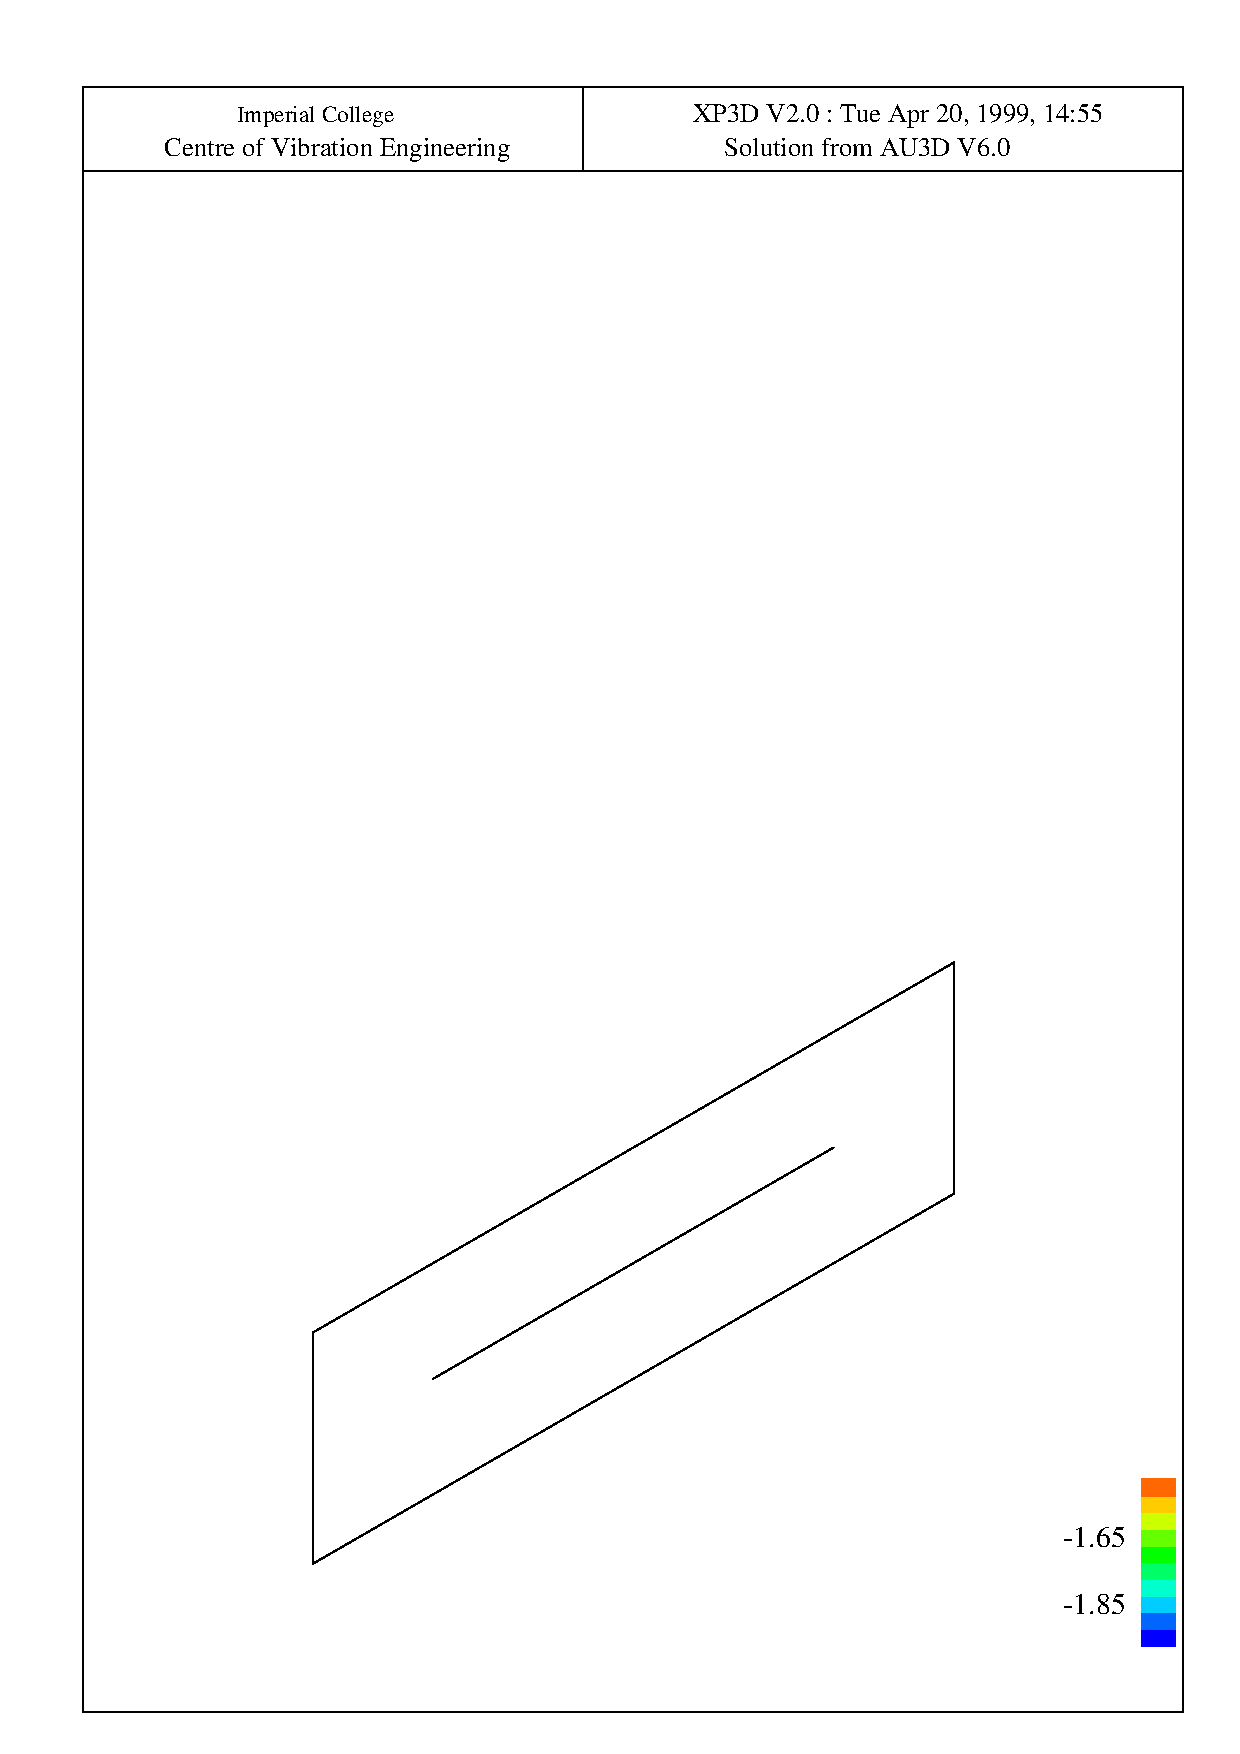
\includegraphics[width=70mm,clip=t]{CHAP_LINEAR/FIGURE/lins_geom.pdf}
       \hspace{0mm}} &
    \subfigure[Computational domain (2,232 points)]
      {\hspace{0mm}
        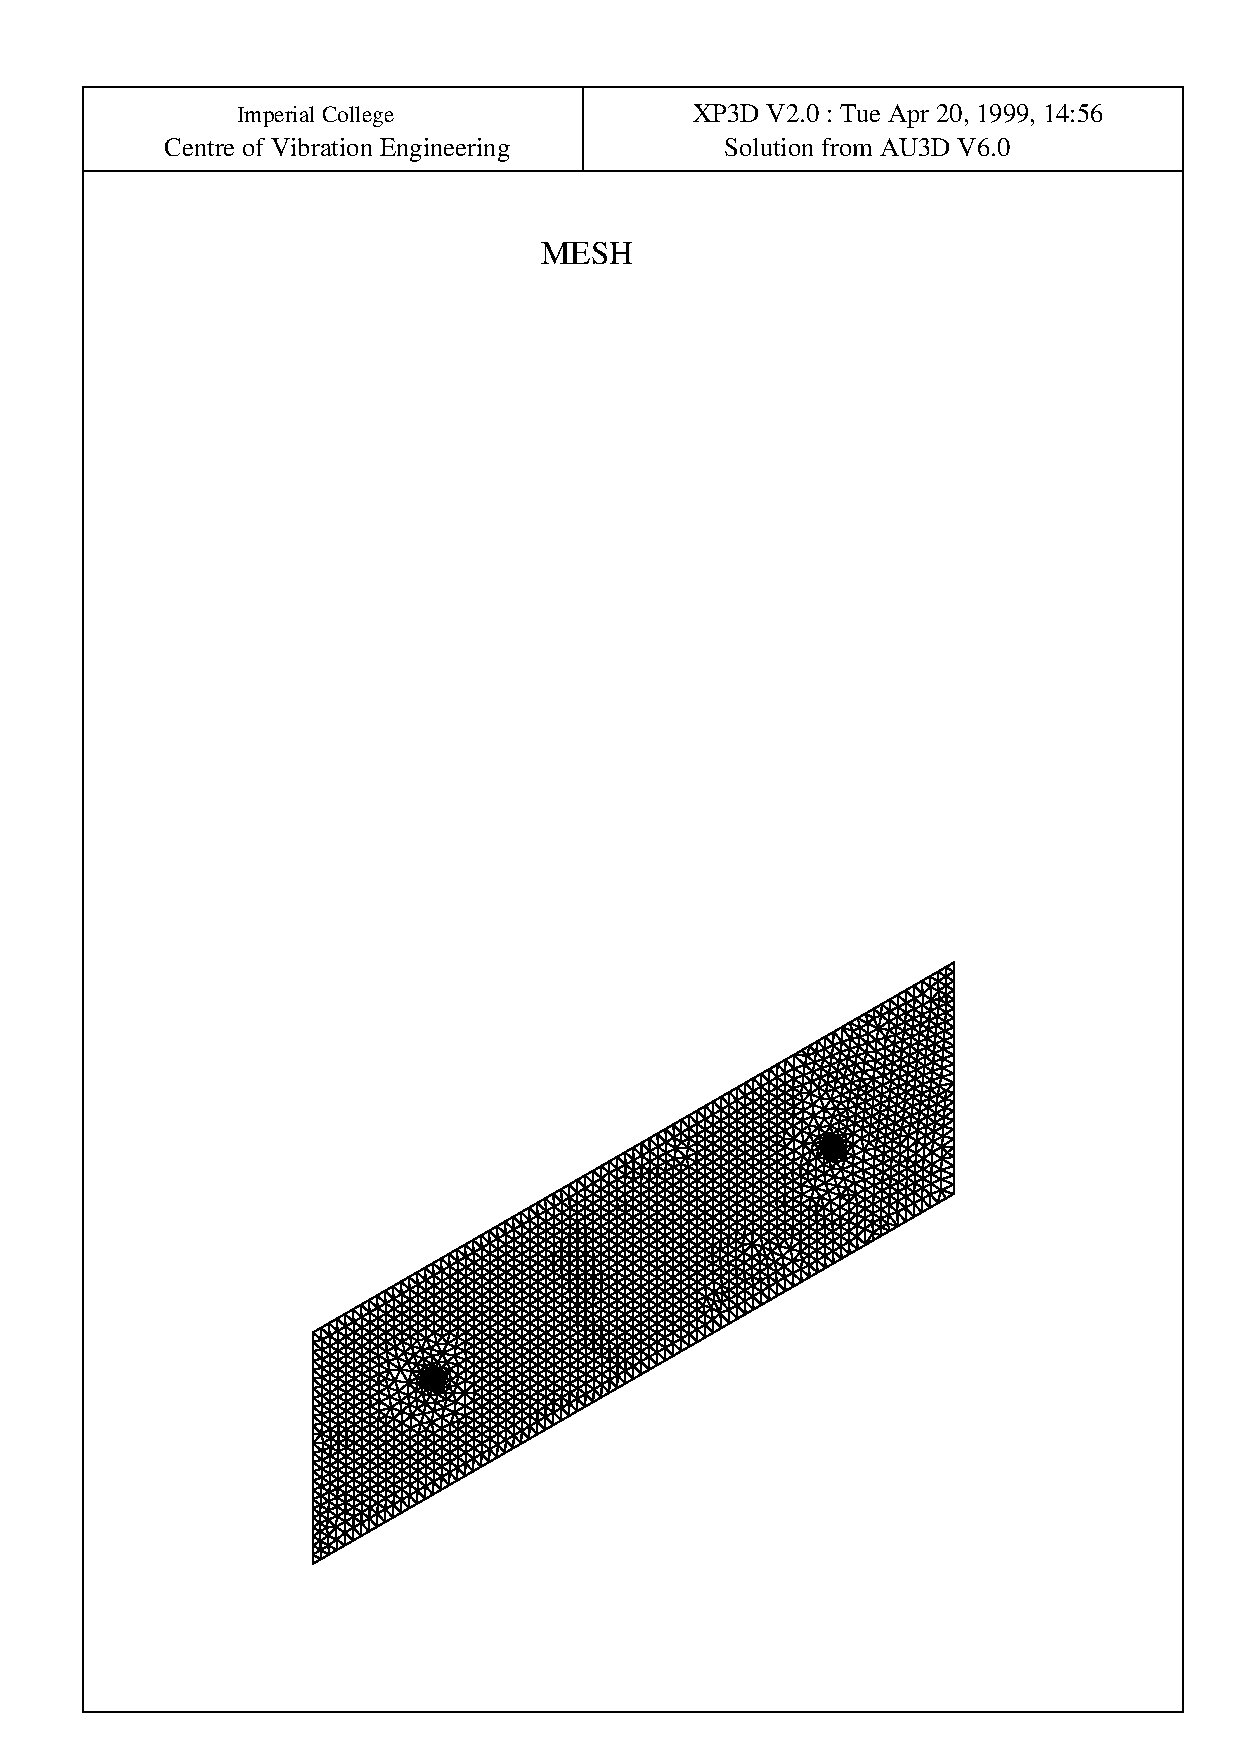
\includegraphics[width=70mm,clip=t]{CHAP_LINEAR/FIGURE/lins_mesh.pdf}}
   \end{tabular}
 \end{center}
 \vspace{-8mm}
 \caption{Flat plate cascade. Geometry and computational domain}
 \label{linsub_geom_mesh.fig}
\end{figure}
%
%
\begin{figure}
  \begin{center}
  \begin{tabular}{c}
    \subfigure[Real part]
       {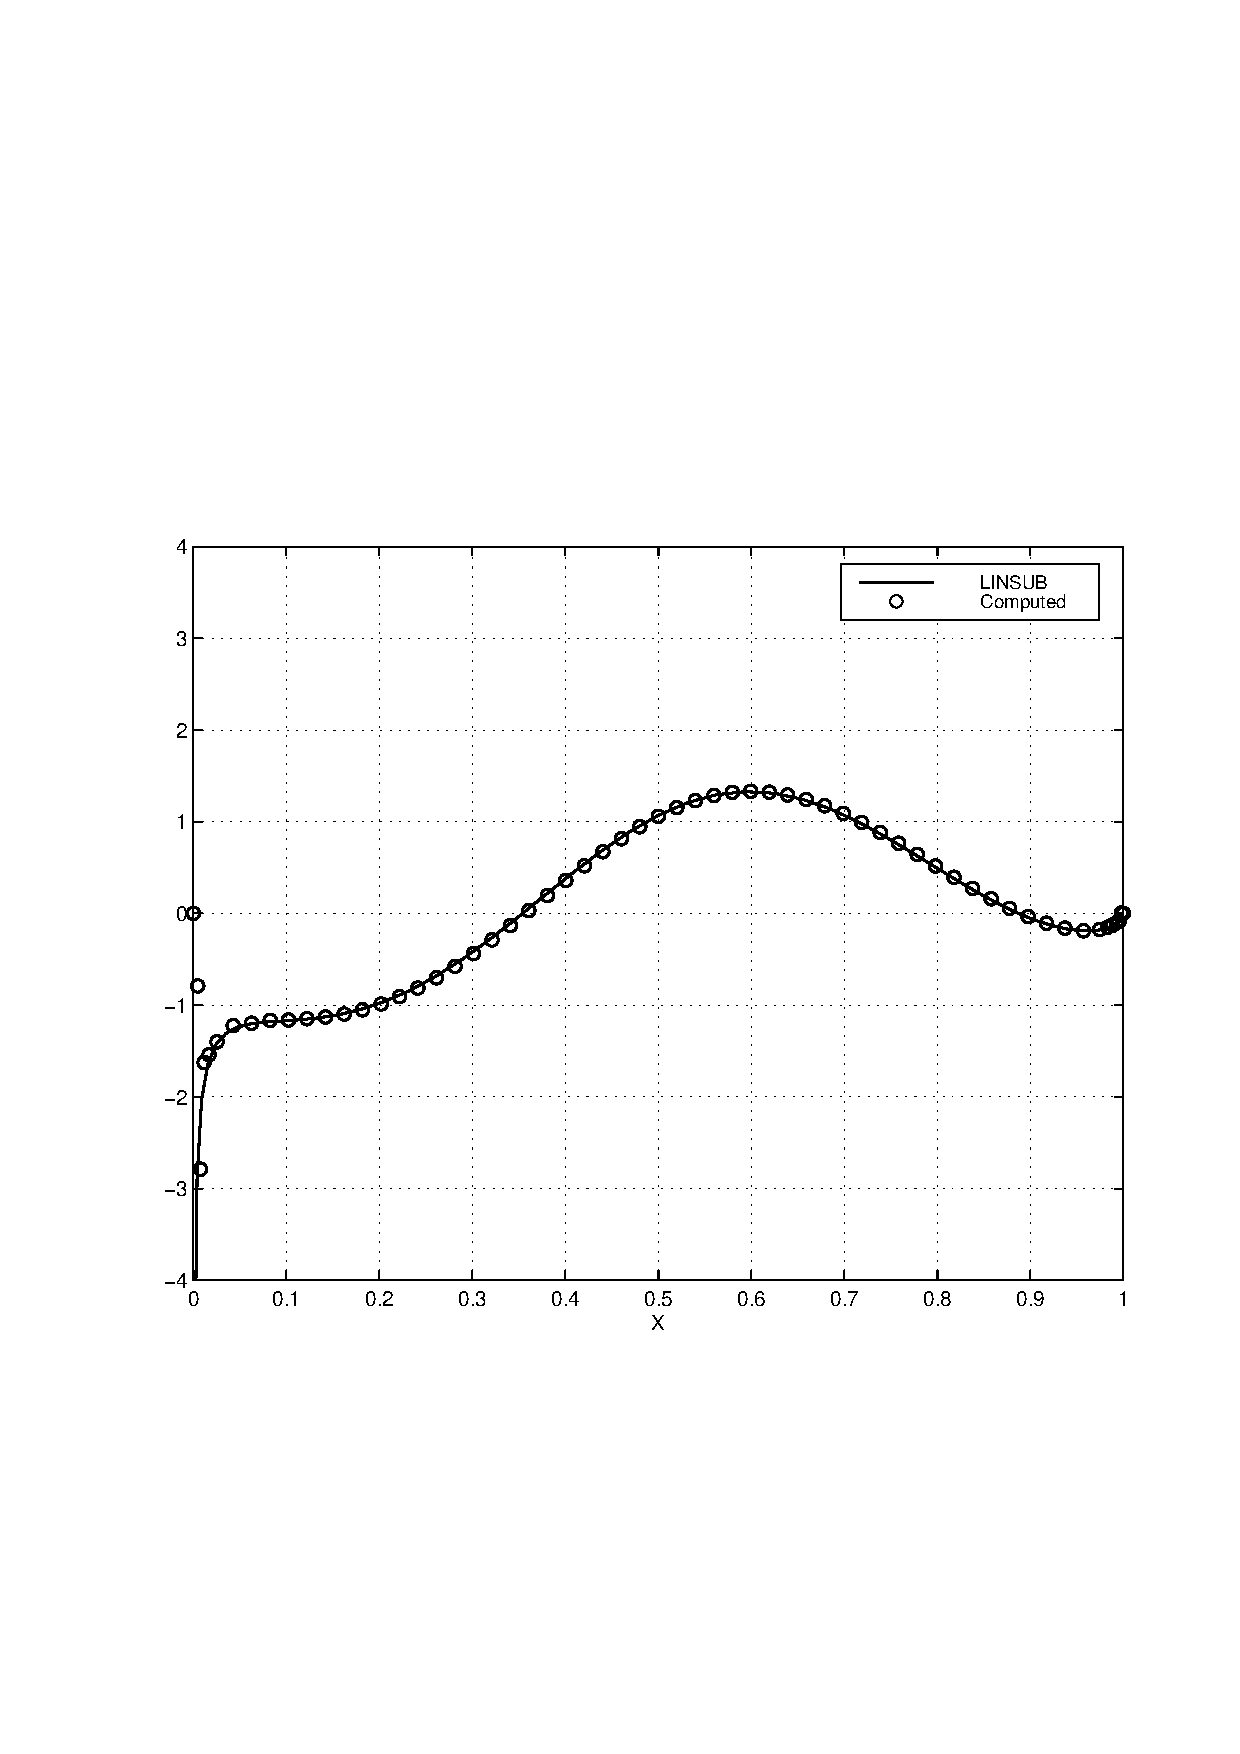
\includegraphics[width=110mm,clip=t]{CHAP_LINEAR/FIGURE/lins_wake1.pdf}
       \hspace{0mm}} \\
    \subfigure[Imaginary part]
      {\hspace{0mm}
        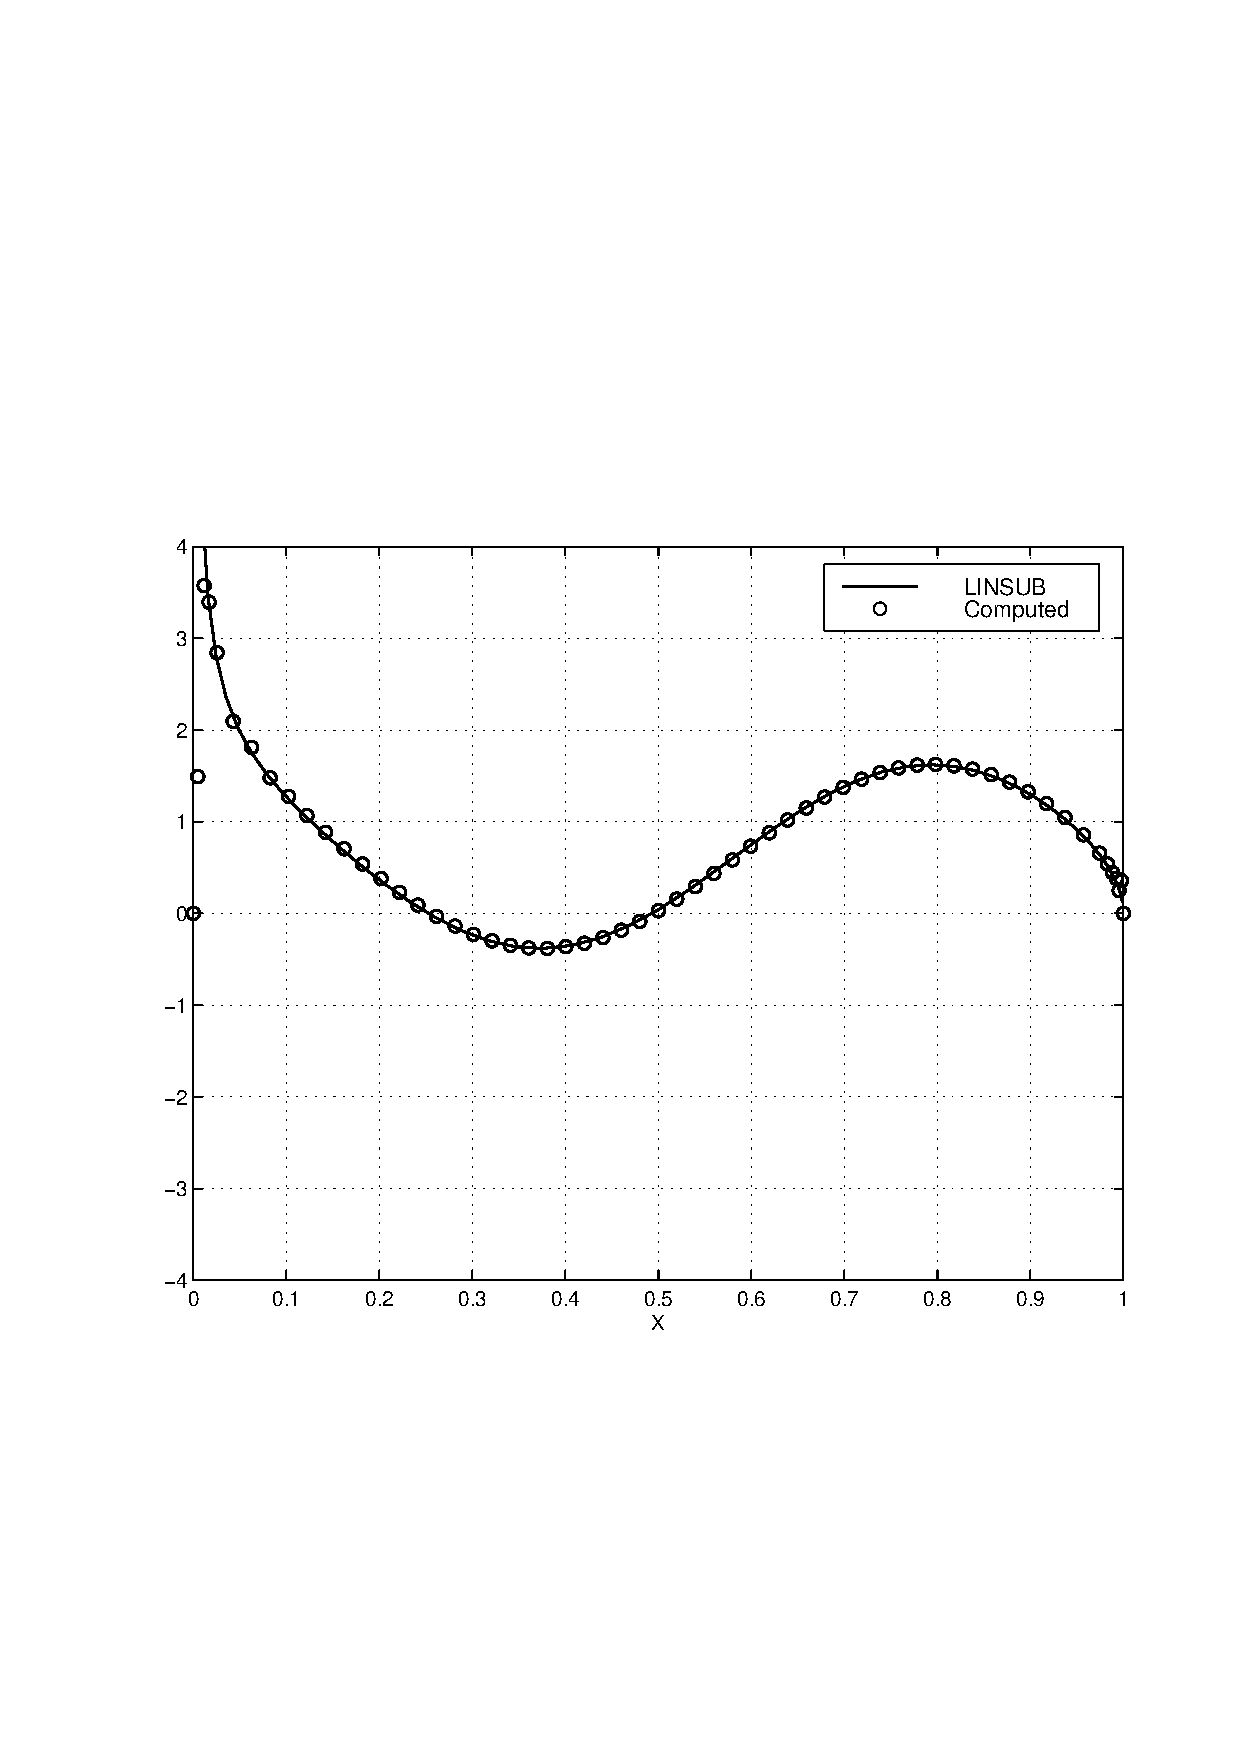
\includegraphics[width=110mm,clip=t]{CHAP_LINEAR/FIGURE/lins_wake2.pdf}}
   \end{tabular}
 \end{center}
 \vspace{-8mm}
 \caption{LINSUB test case. Pressure jump on flat plate due to wake/rotor interaction
          ($\omega = \pi$, $\phi = -90\se{o}$)}
 \label{linsub_wake.fig}
\end{figure}
%
\begin{figure}
  \begin{center}
  \begin{tabular}{c}
    \subfigure[Real part]
       {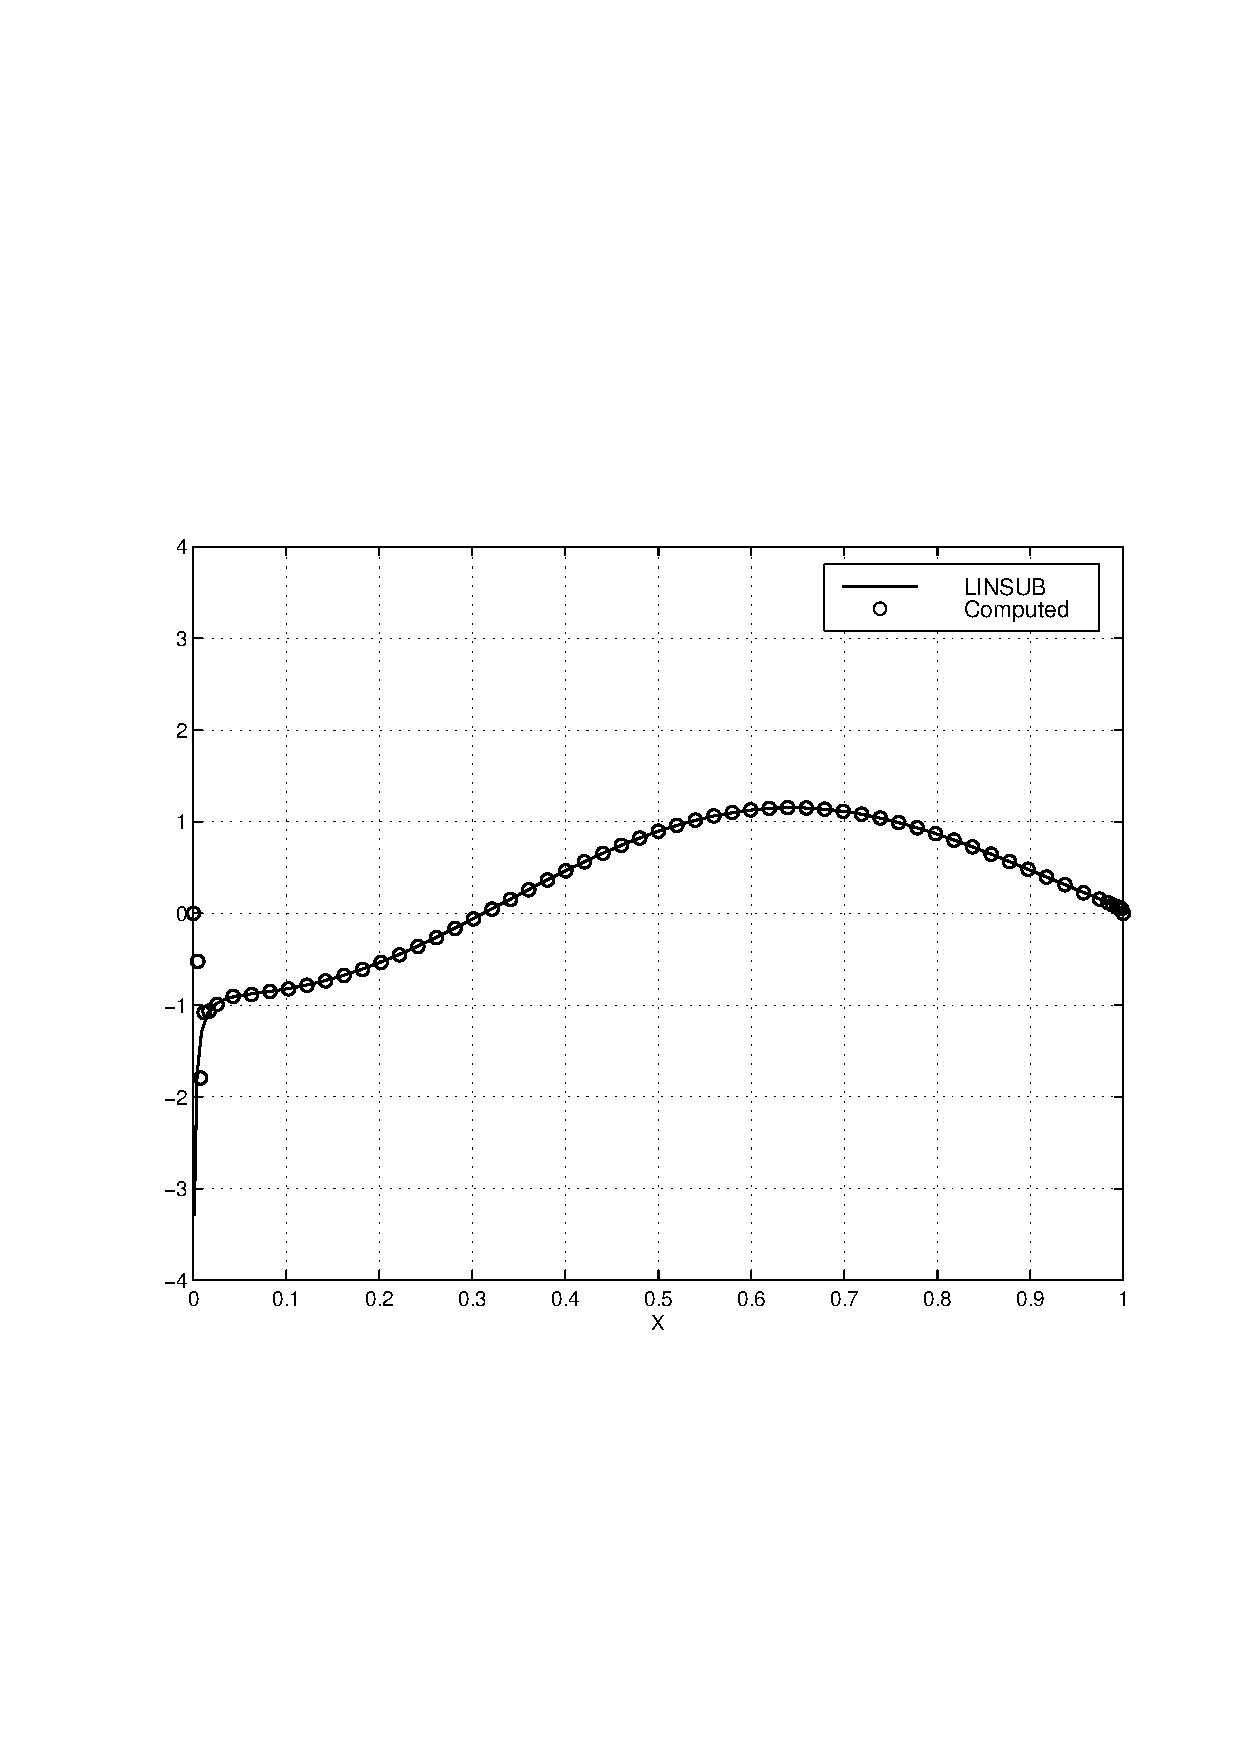
\includegraphics[width=110mm,clip=t]{CHAP_LINEAR/FIGURE/lins_pres1.pdf}
       \hspace{0mm}} \\
    \subfigure[Imaginary part]
      {\hspace{0mm}
        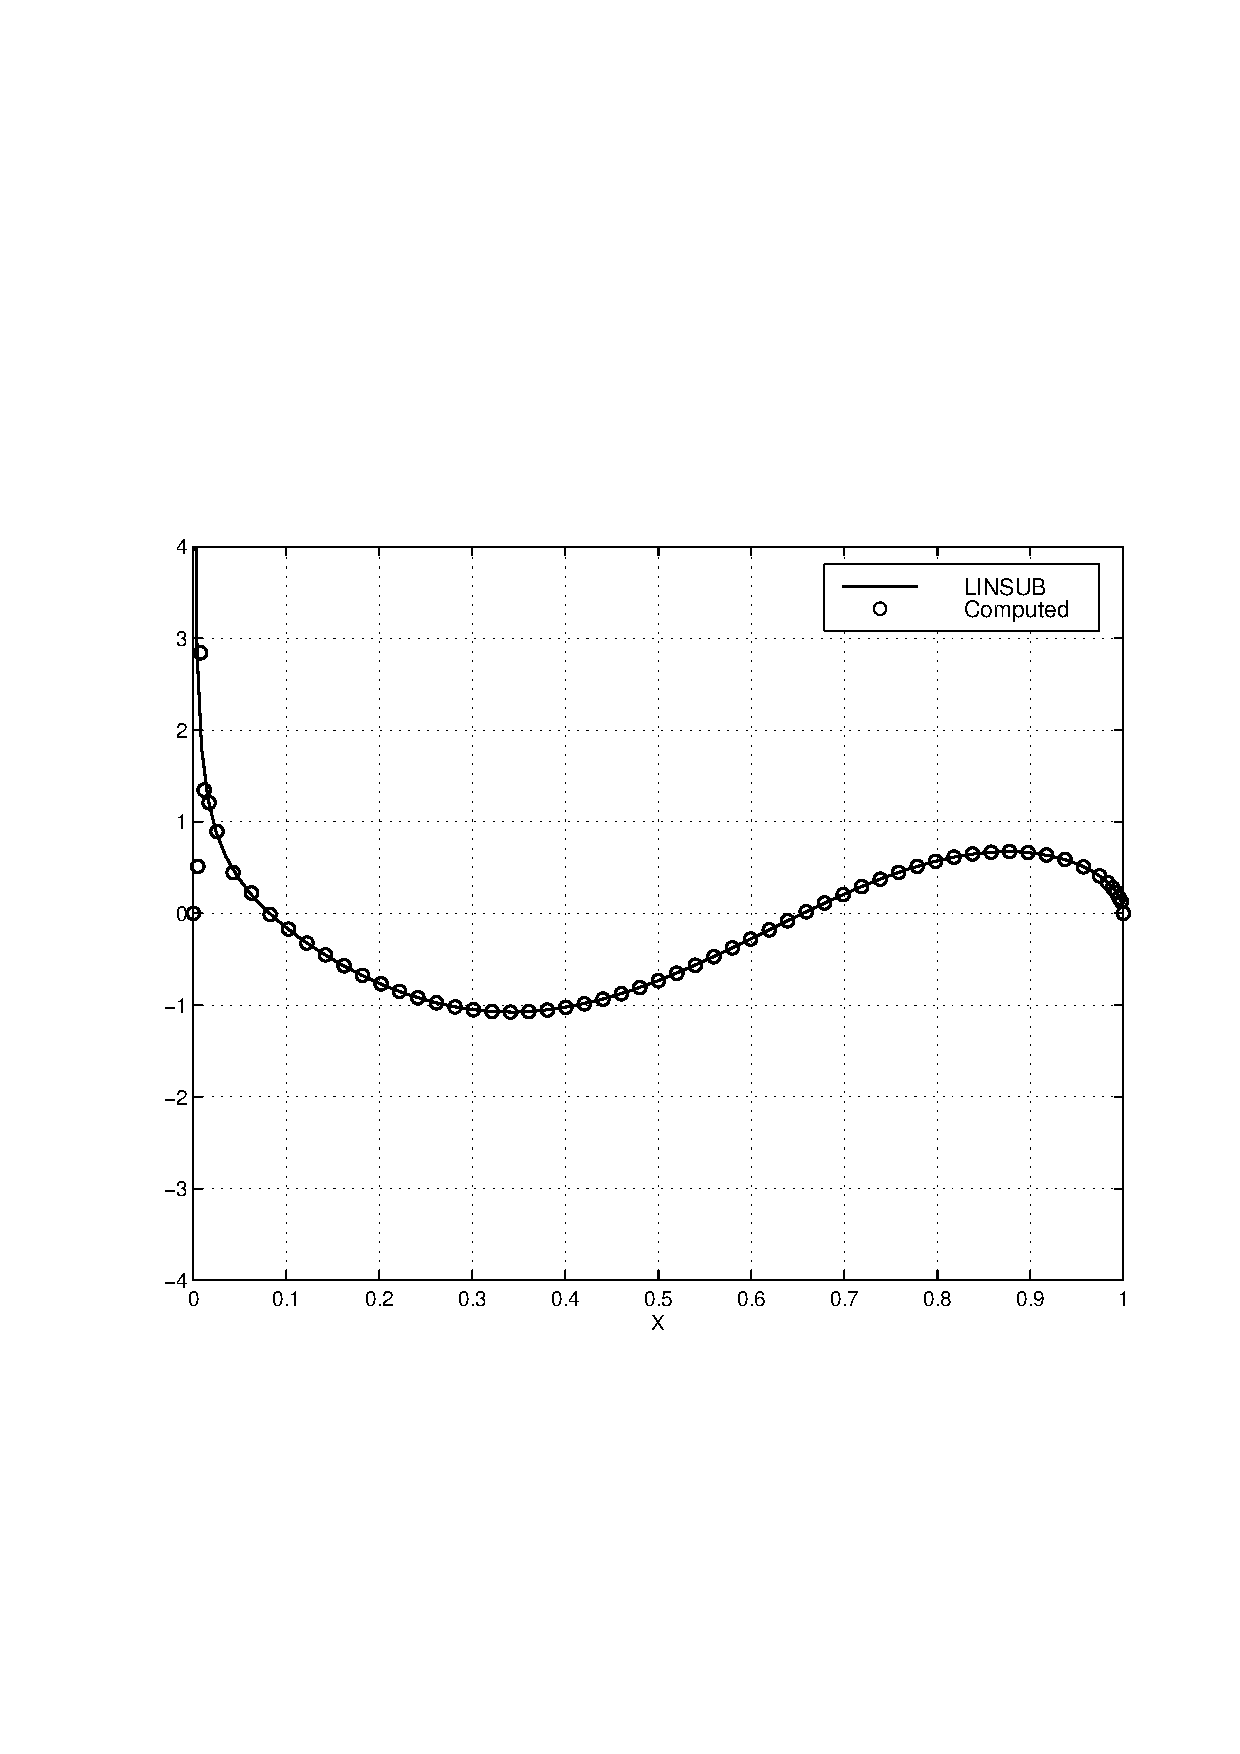
\includegraphics[width=110mm,clip=t]{CHAP_LINEAR/FIGURE/lins_pres2.pdf}}
   \end{tabular}
 \end{center}
 \vspace{-8mm}
 \caption{LINSUB test case. Pressure jump on flat plate due to upstream acoustic wave
          ($\omega = 2$, $\phi = 0\se{o}$)}
 \label{linsub_pres.fig}
\end{figure}
%
\begin{figure}
  \begin{center}
  \begin{tabular}{c}
    \subfigure[Real part]
       {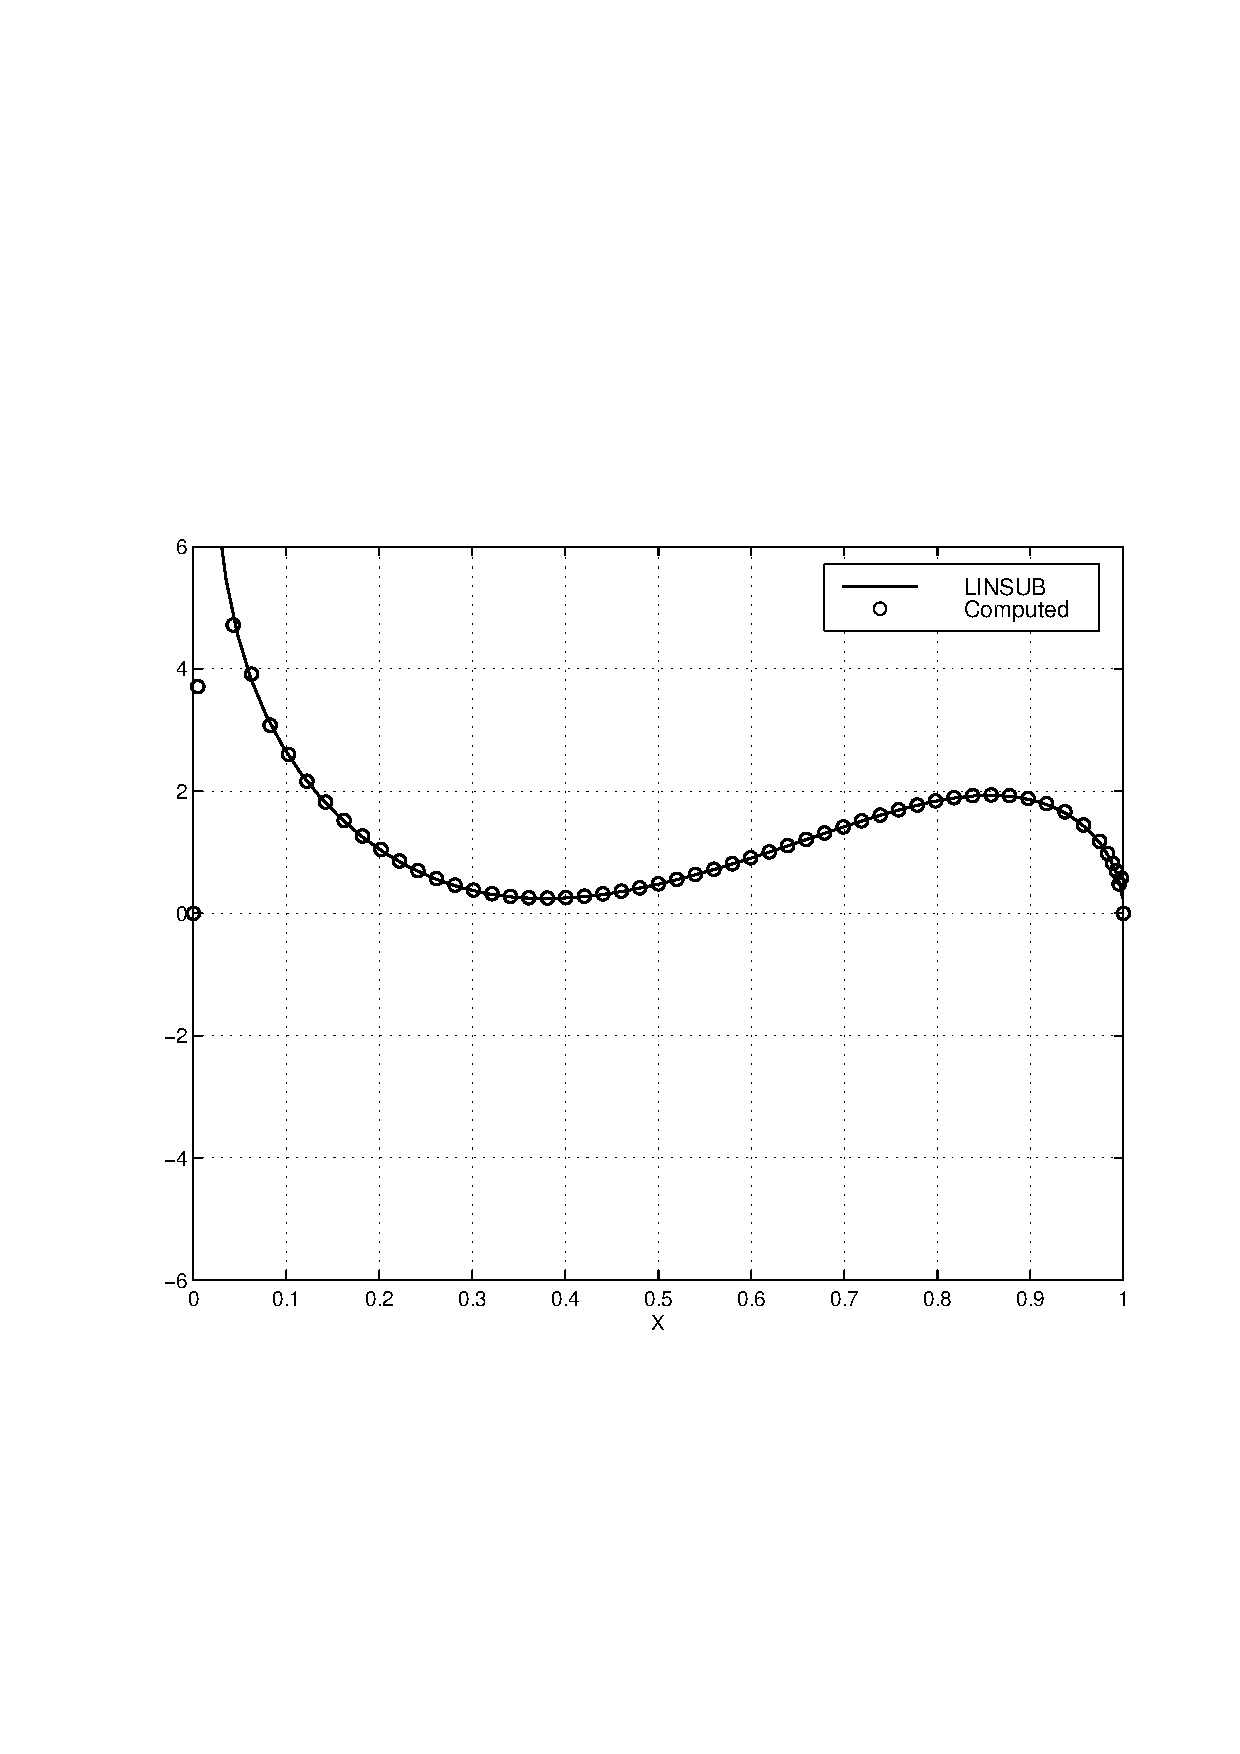
\includegraphics[width=110mm,clip=t]{CHAP_LINEAR/FIGURE/lins_bend1.pdf}
       \hspace{0mm}} \\
    \subfigure[Imaginary part]
      {\hspace{0mm}
        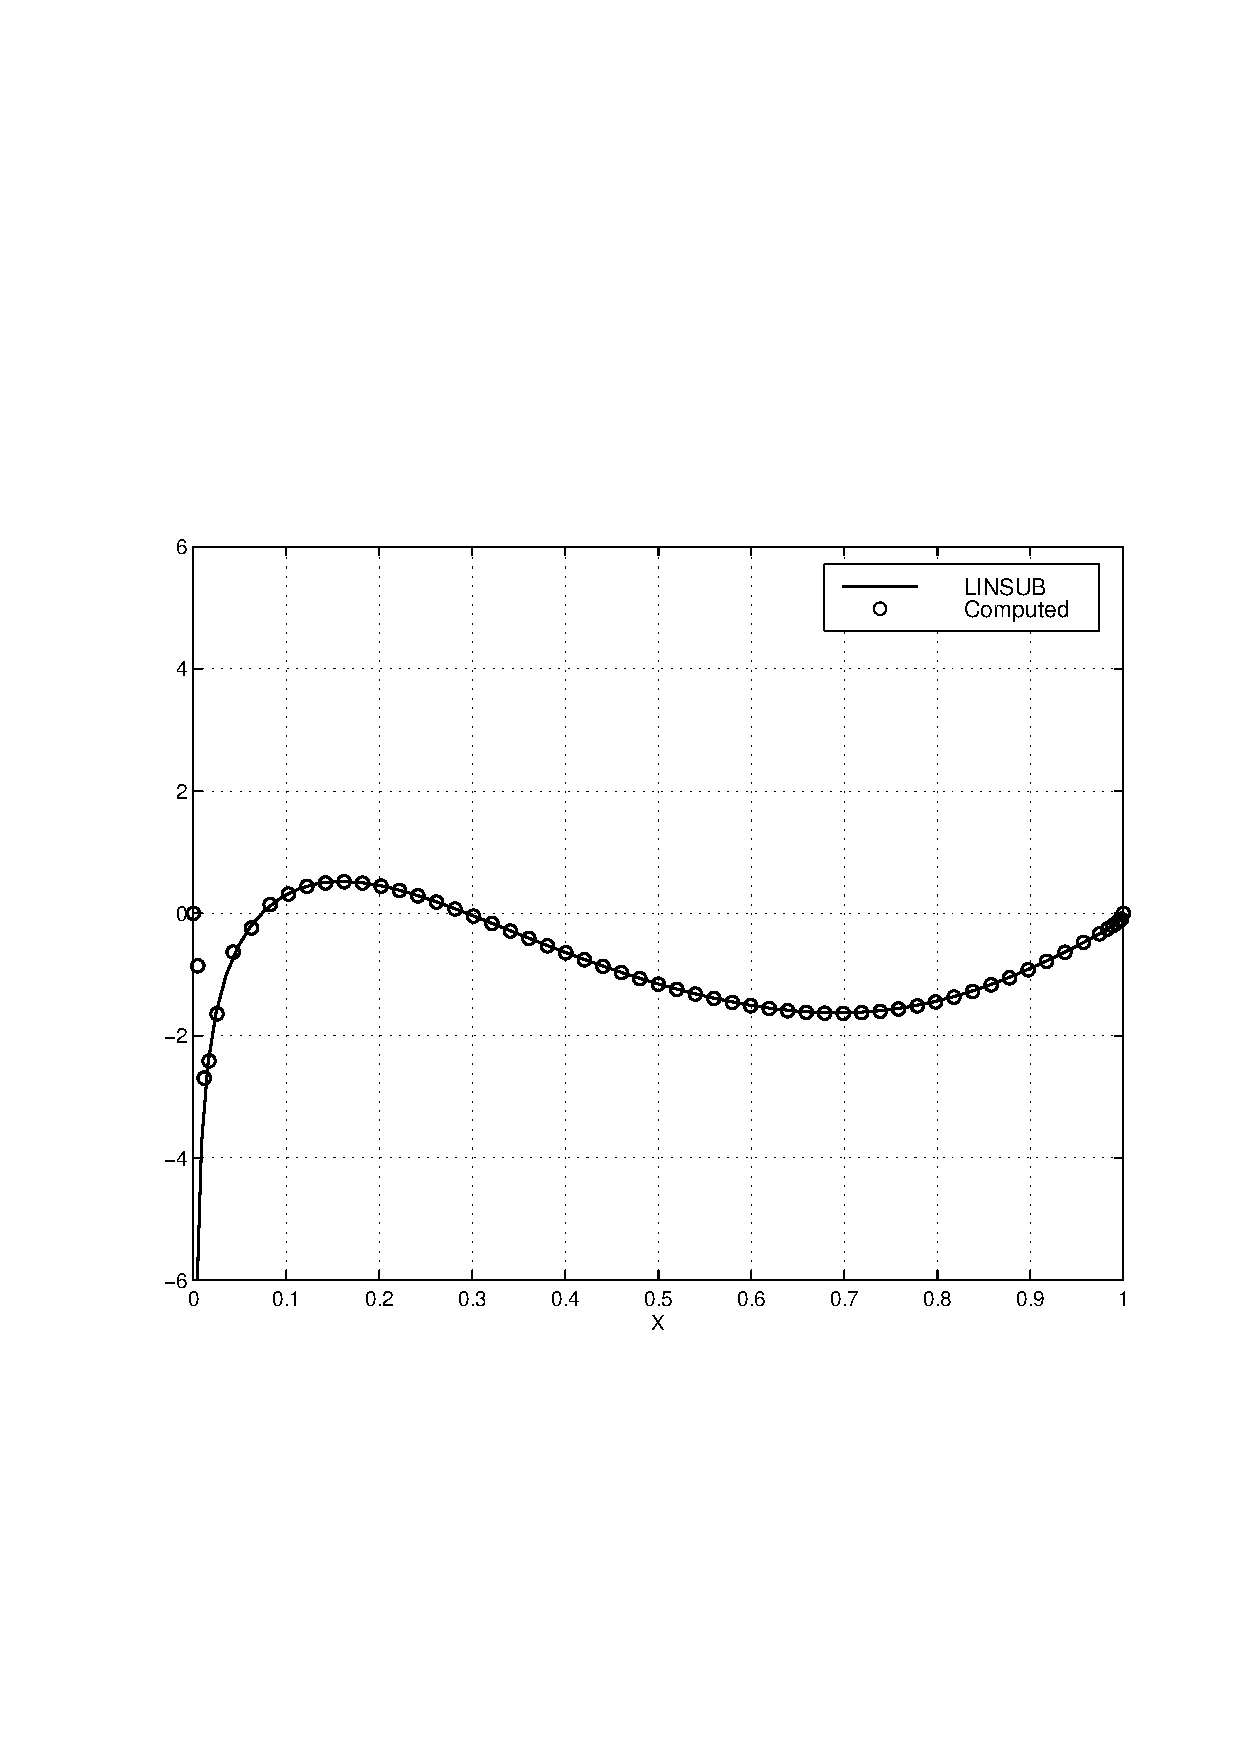
\includegraphics[width=110mm,clip=t]{CHAP_LINEAR/FIGURE/lins_bend2.pdf}}
   \end{tabular}
 \end{center}
 \vspace{-8mm}
 \caption{LINSUB test case. Pressure jump on flat plate due to bending oscillation
          ($\omega = 2$, $\phi = 90\se{o}$)}
 \label{linsub_bend.fig}
\end{figure}
%
%
 Small-amplitude perturbations of a uniform, inviscid steady-state flow past an
 unloaded flat-plate cascade are studied first.  Such cascades can  be used for a
 variety of applications: wake/blade interaction, potential/blade interaction, aeroelasticity
 studies by including the blade's bending and torsional motion. The main aerodynamic
 parameters are the Mach number, reduced frequency, pitch-to-chord ratio, stagger
 angle and the interblade phase angle.

 Three different disturbances were studied for  a pitch-to-chord ratio of 0.5,
 a stagger angle of $30\se{o}$ and a mean-flow Mach number of 0.7.
 For all three cases, the results were checked against the benchmark LINSUB code
 by plotting the real and imaginary parts of the (complex) unsteady pressure difference across
 the plate.  The geometry and the computational domain  are
 shown in Fig. \ref{linsub_geom_mesh.fig}. The mesh has high resolution around the
 trailing and leading edges in order to handle the singularities which occur
 in these regions.

 The first disturbance simulates a wake/blade interaction, an incoming
 sinusoidal wake with a reduced frequency of $\pi$ being specified at the inflow boundary.
 The  interblade phase angle is $-90\se{o}$. Fig. \ref{linsub_wake.fig}
 shows  excellent agreement between the present method and the benchmark program LINSUB.
 The second disturbance simulates potential/blade interaction,  an
 incoming pressure wave with a reduced frequency of $2.0$ being specified
 at the outflow boundary. The interblade phase angle is $0\se{o}$.
 Fig. \ref{linsub_pres.fig} shows excellent agreement between the present method and the
 benchmark program LINSUB.
 The last disturbance  studied is for a bending motion with a reduced frequency of
 $2.0$ and an interblade phase angle of $90\se{o}$. Once again, excellent agreement
 is observed from Fig. \ref{linsub_bend.fig}.
%

%
%
%
\subsection{Unsteady laminar boundary layer on a flat plate}
\label{unsteady_flat_linear.subsec}
%
\begin{figure}
  \begin{center}
  \begin{tabular}{cc}
    \subfigure[Computational mesh (5954 points)]
       {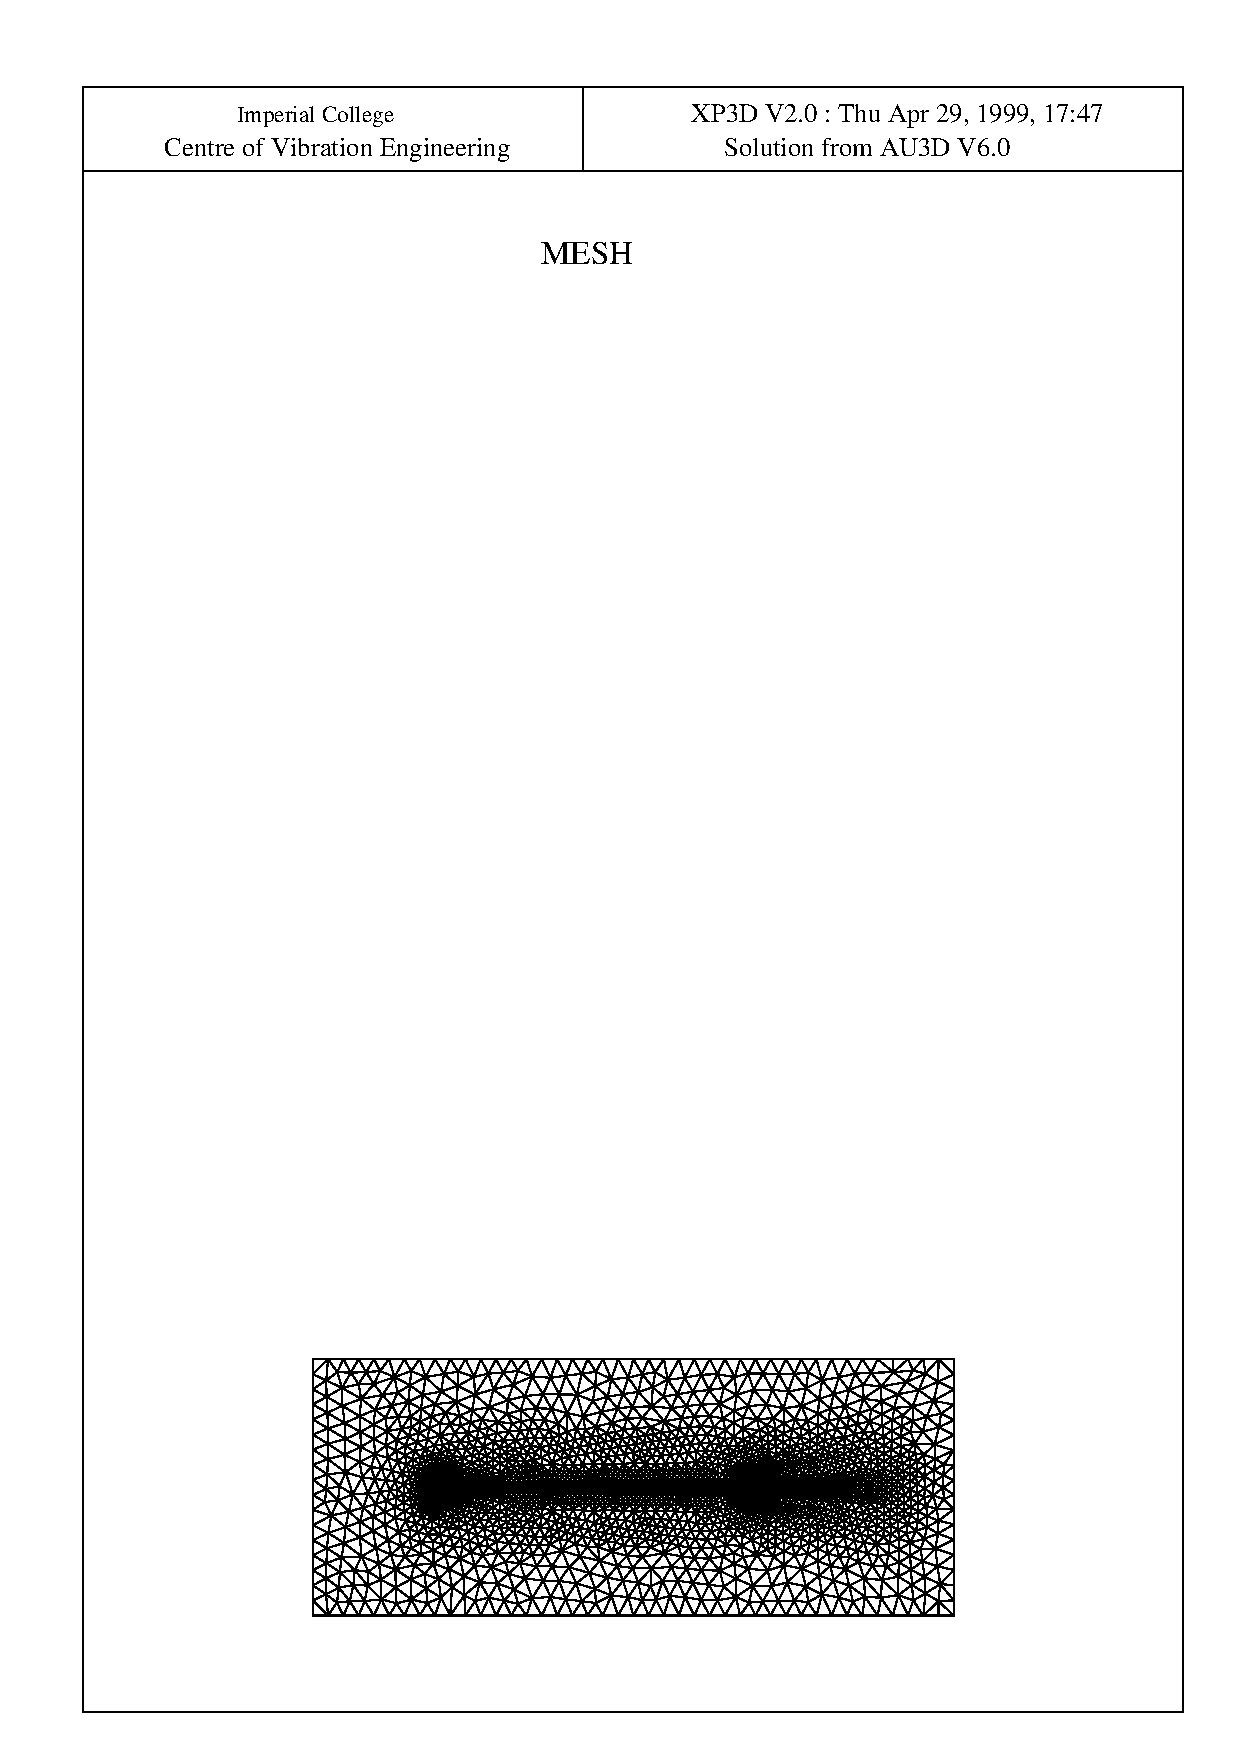
\includegraphics[width=80mm,clip=t]{CHAP_LINEAR/FIGURE/flat_laminar_mesh1.pdf}
       \hspace{0mm}} &
    \subfigure[trailing edge]
      {\hspace{0mm}
        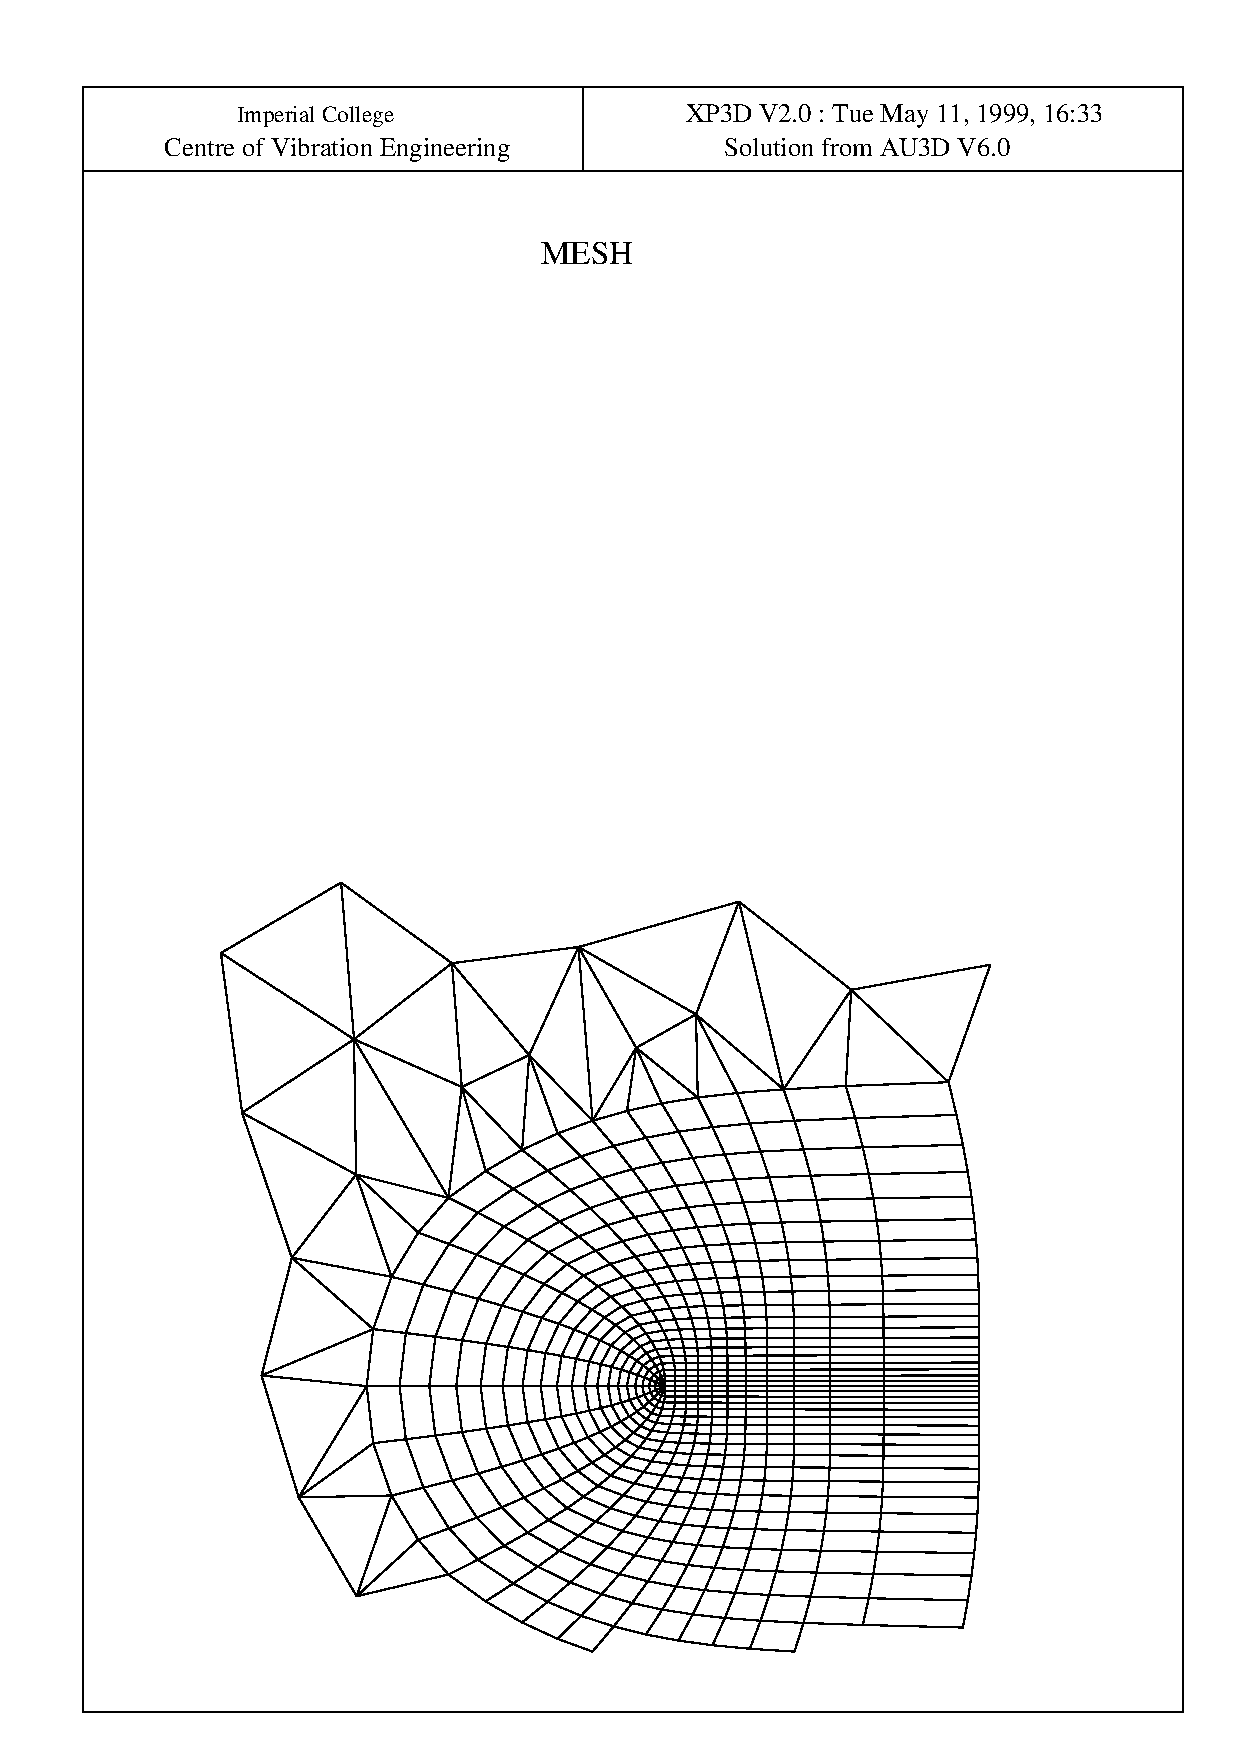
\includegraphics[width=40mm,clip=t]{CHAP_LINEAR/FIGURE/flat_laminar_mesh2.pdf}}
   \end{tabular}
 \end{center}
 \vspace{-7mm}
 \caption{Computational domain for laminar flow over a flat plate cascade}
 \label{flat_laminar_linear_mesh.fig}
\end{figure}
%
 This test case studies an unsteady laminar
 boundary layer with fluctuations in external velocity.
 The computational mesh is shown in Fig. \ref{flat_laminar_linear_mesh.fig}.
 The boundary layer region is discretised using 15 layers of quadrilateral elements,
 while the rest of the domain consists of triangles.
 The pitch to chord ratio of this cascade is unity so that the flow is
 as close as possible to that over an isolated flat plate.
 The steady-state flow  over an unstaggered flat plate cascade was obtained for
 a Mach number of 0.2.  The freestream Reynolds number is 60,000. Such a case is
 well within the incompressible flow regime, thus enabling  a meaningful comparison
 with the Blasius solution.  Indeed, the computed steady-state  velocity profile and
 the skin friction coefficient are found to be in very good agreement with the
 incompressible laminar boundary layer theory of  Blasius (Fig. \ref{flat_laminar_steady.fig}).
 Once the steady-state flow has been validated, the next stage is to study a
 velocity perturbation of the form:

%
\beq
  u = \varepsilon u\sm{\infty} e\se{-i\omega t}
\eeq
%
 where $u\sm{\infty}$ is the freestream velocity and $\varepsilon$ a small value ($\ll 1$).
 The disturbance is along the plate, in the freestream direction, denoted by co-ordinate $x$.
 Lighthill's \citeyear{Lighthill:1} theory provides two asymptotic values for
 the unsteady skin friction coefficient, one for very small and the other for very
 large reduced frequency values. Fig. \ref{flat_laminar_linear_sol.fig}a
 shows the wall shear stress amplitude variation with reduced frequency $\omega x/u\sm{\infty}$
 while Fig. \ref{flat_laminar_linear_sol.fig}b shows the computed phase angle
 between shear stress and external velocity. As expected, the computed results
 become asymptotic for the limiting cases of very small and very large reduced
 frequency. Similar comparisons between numerical results and Lighthill's theory
 are also reported by Cebeci \citeyear{Cebeci:1}.
%
%
%
\begin{figure}
  \begin{center}
  \begin{tabular}{c}
    \subfigure[Velocity profile]
       {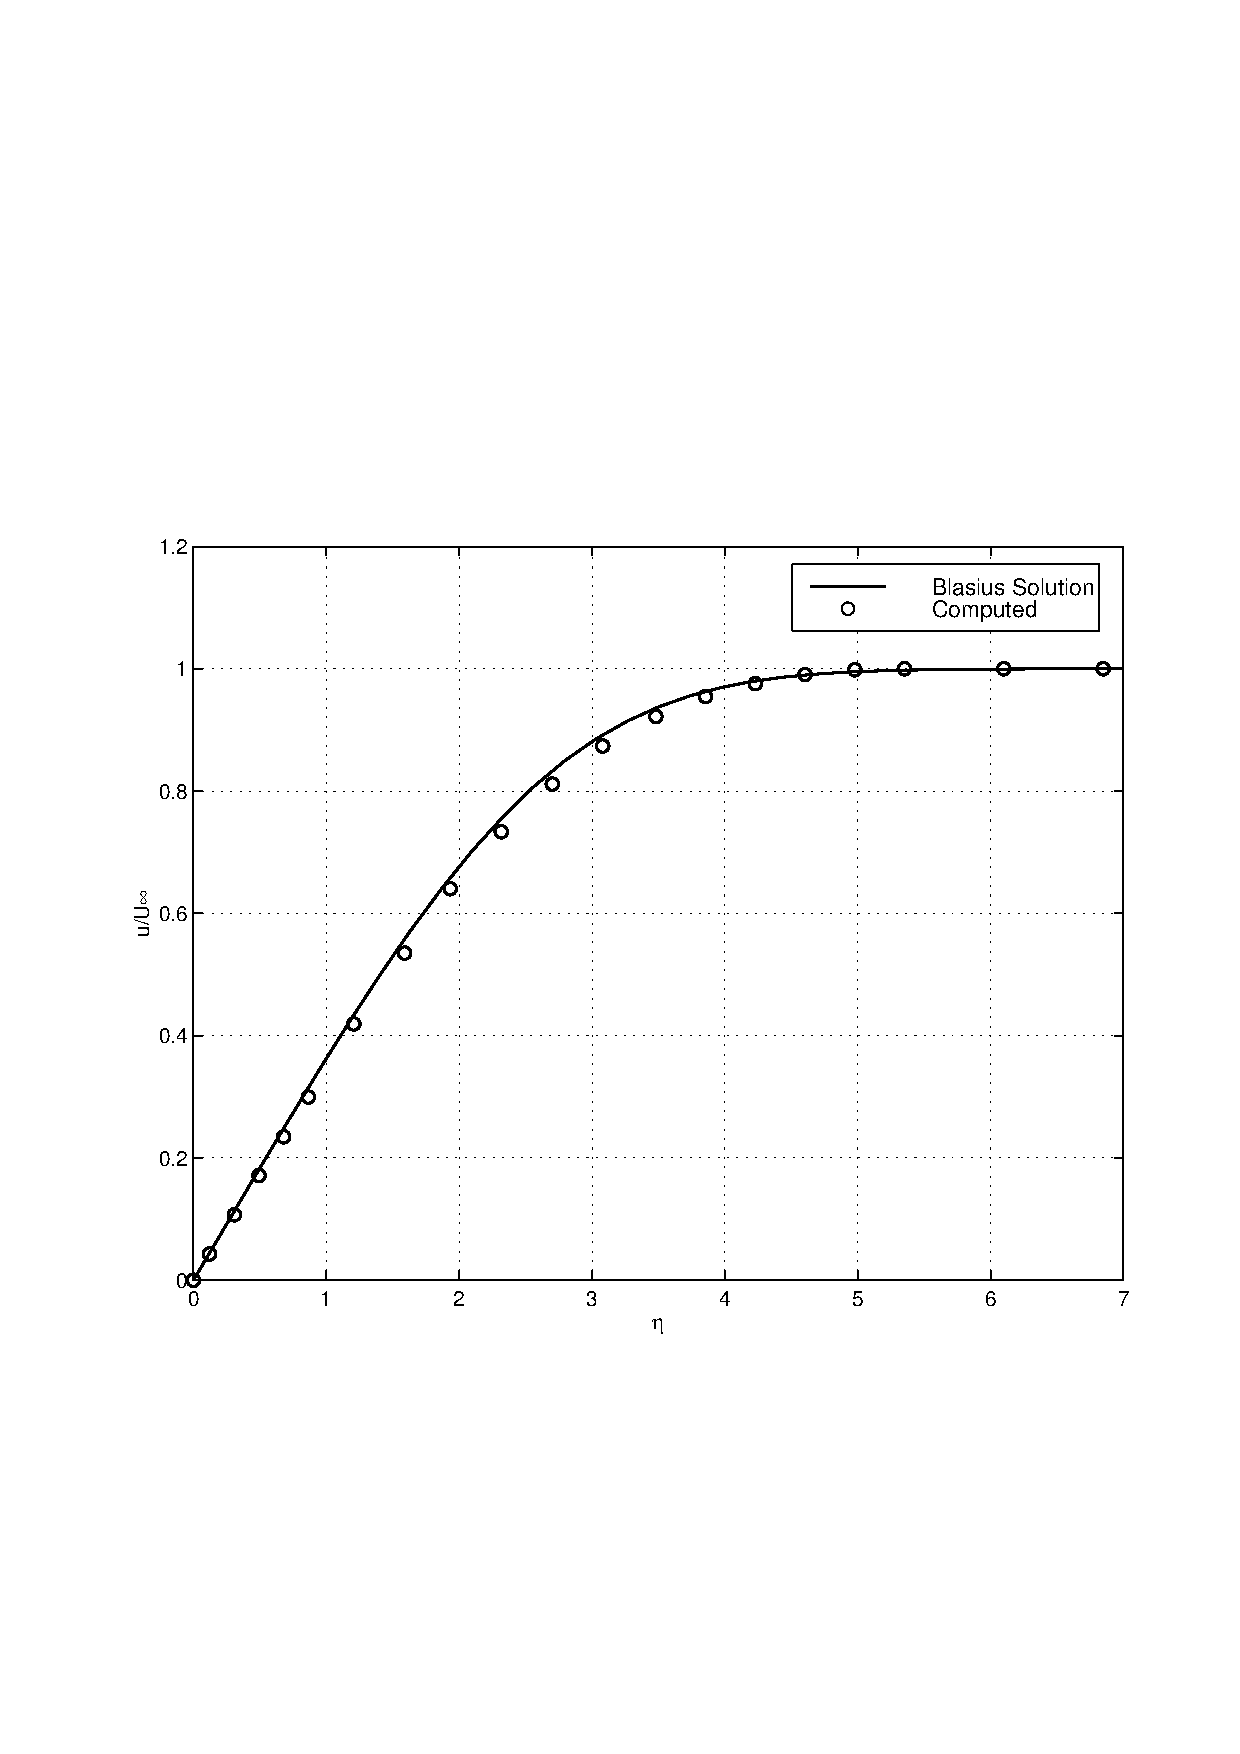
\includegraphics[width=110mm,clip=t]{CHAP_LINEAR/FIGURE/flat_laminar_vel.pdf}
       \hspace{0mm}} \\
    \subfigure[Skin friction coefficient]
      {\hspace{0mm}
        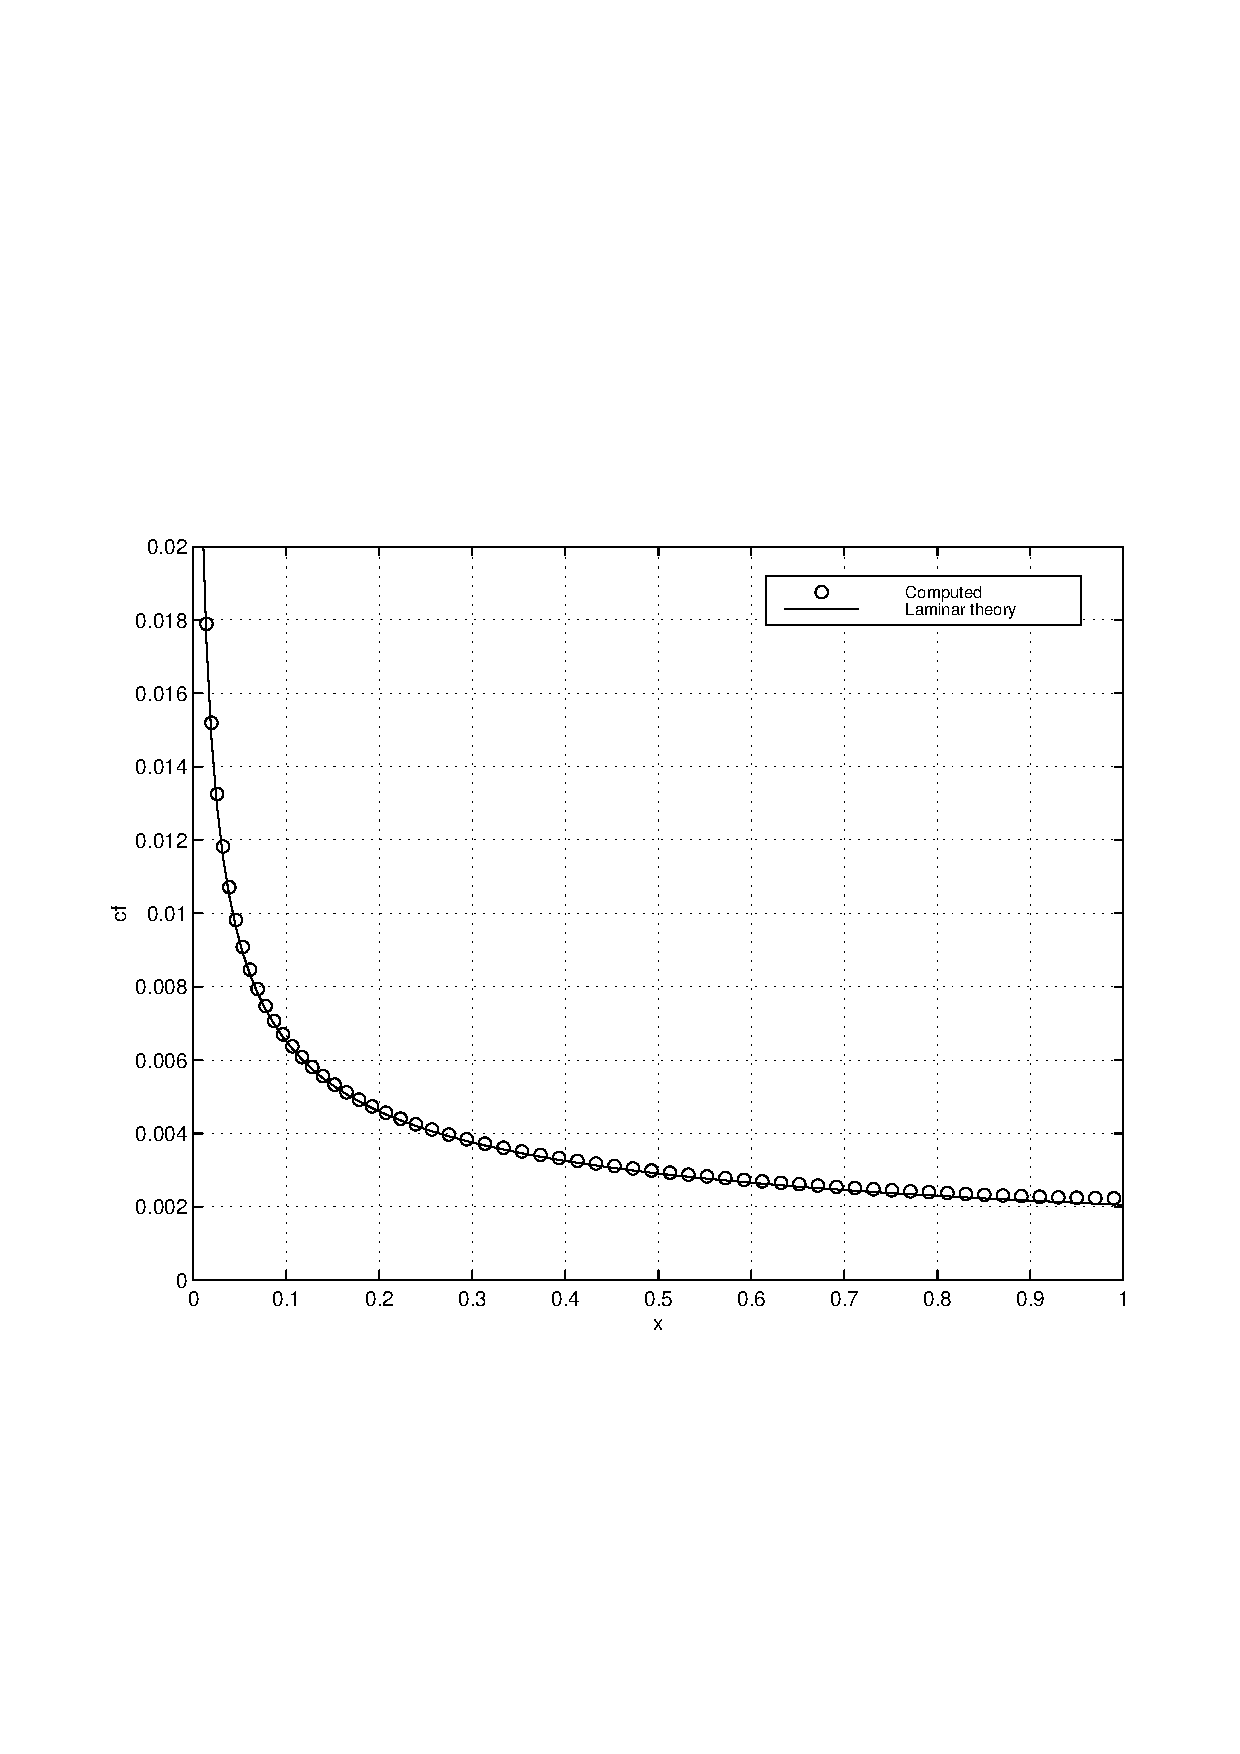
\includegraphics[width=110mm,clip=t]{CHAP_LINEAR/FIGURE/flat_laminar_cff.pdf}}
   \end{tabular}
 \end{center}
 \vspace{-7mm}
 \caption{Steady laminar flow over a cascade of flat plates}
 \label{flat_laminar_steady.fig}
\end{figure}
%
\begin{figure}
  \begin{center}
   \begin{tabular}{c}
    \subfigure[Amplitude]
       {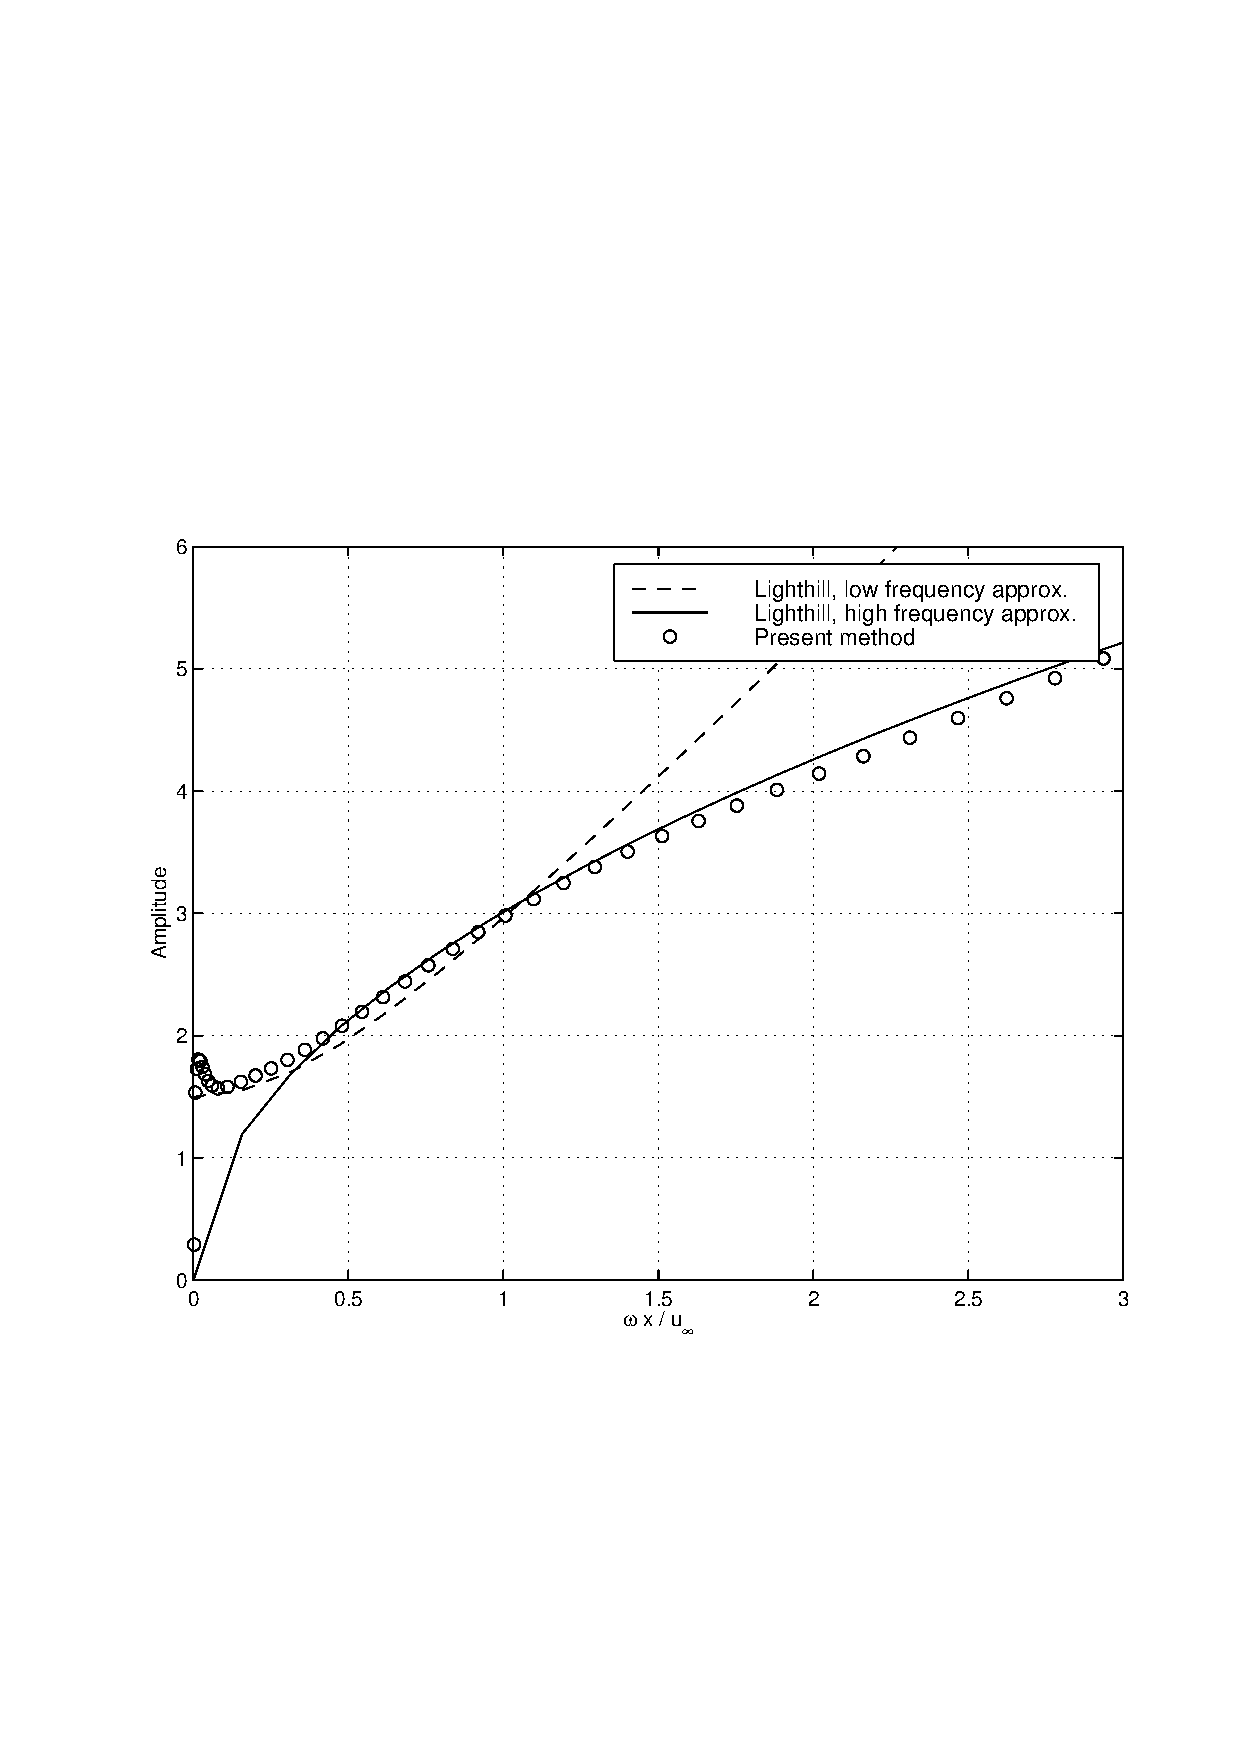
\includegraphics[width=110mm,clip=t]{CHAP_LINEAR/FIGURE/flat_laminar_ampli.pdf}
       \hspace{0mm}} \\
    \subfigure[Phase angle with respect to external velocity fluctuation]
      {\hspace{0mm}
        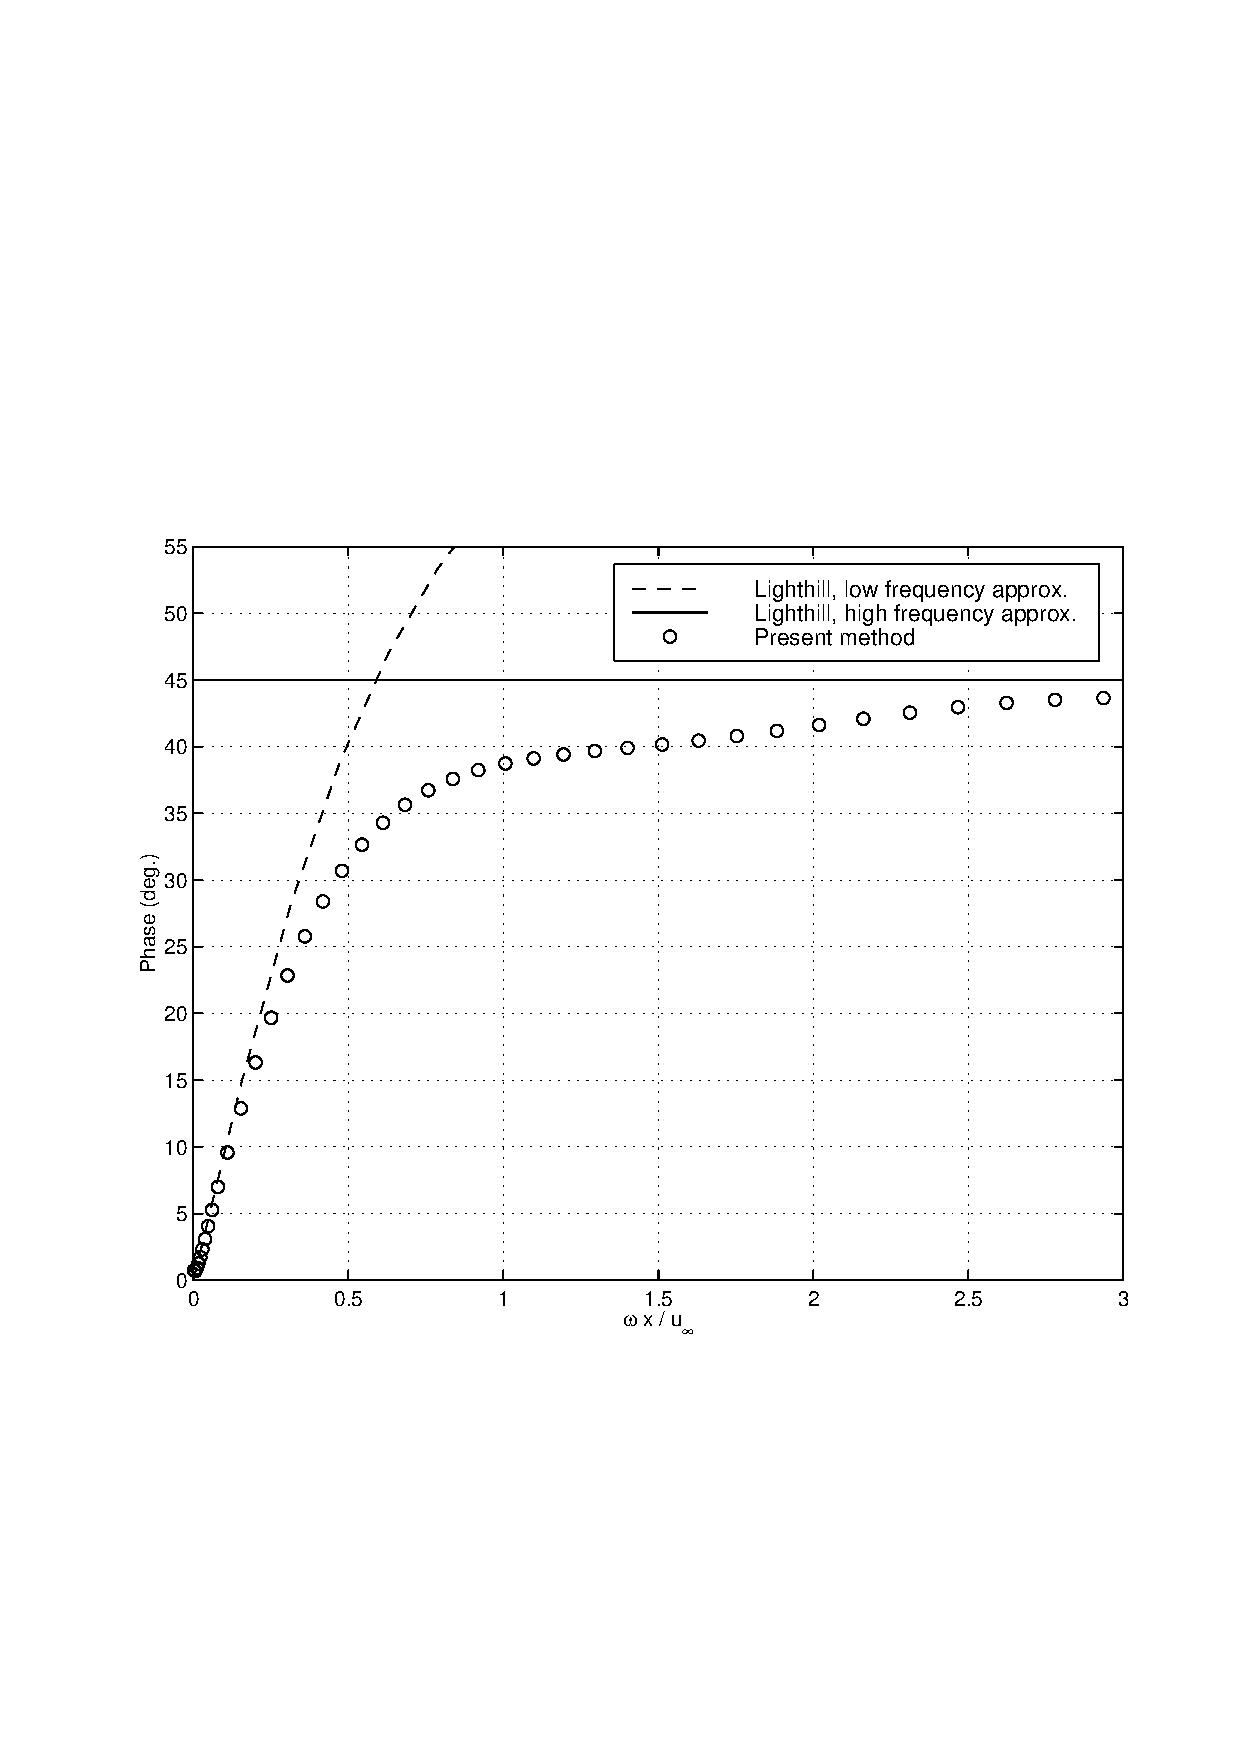
\includegraphics[width=110mm,clip=t]{CHAP_LINEAR/FIGURE/flat_laminar_phase.pdf}}
   \end{tabular}
 \end{center}
 \vspace{-7mm}
 \caption{Unsteady wall shear stresses for an oscillating laminar boundary layer}
 \label{flat_laminar_linear_sol.fig}
\end{figure}
%

%
%
%
%
\subsection{Turbine cascade}
\label{stand11.subsec}
%
%
\begin{figure}
 \centerline{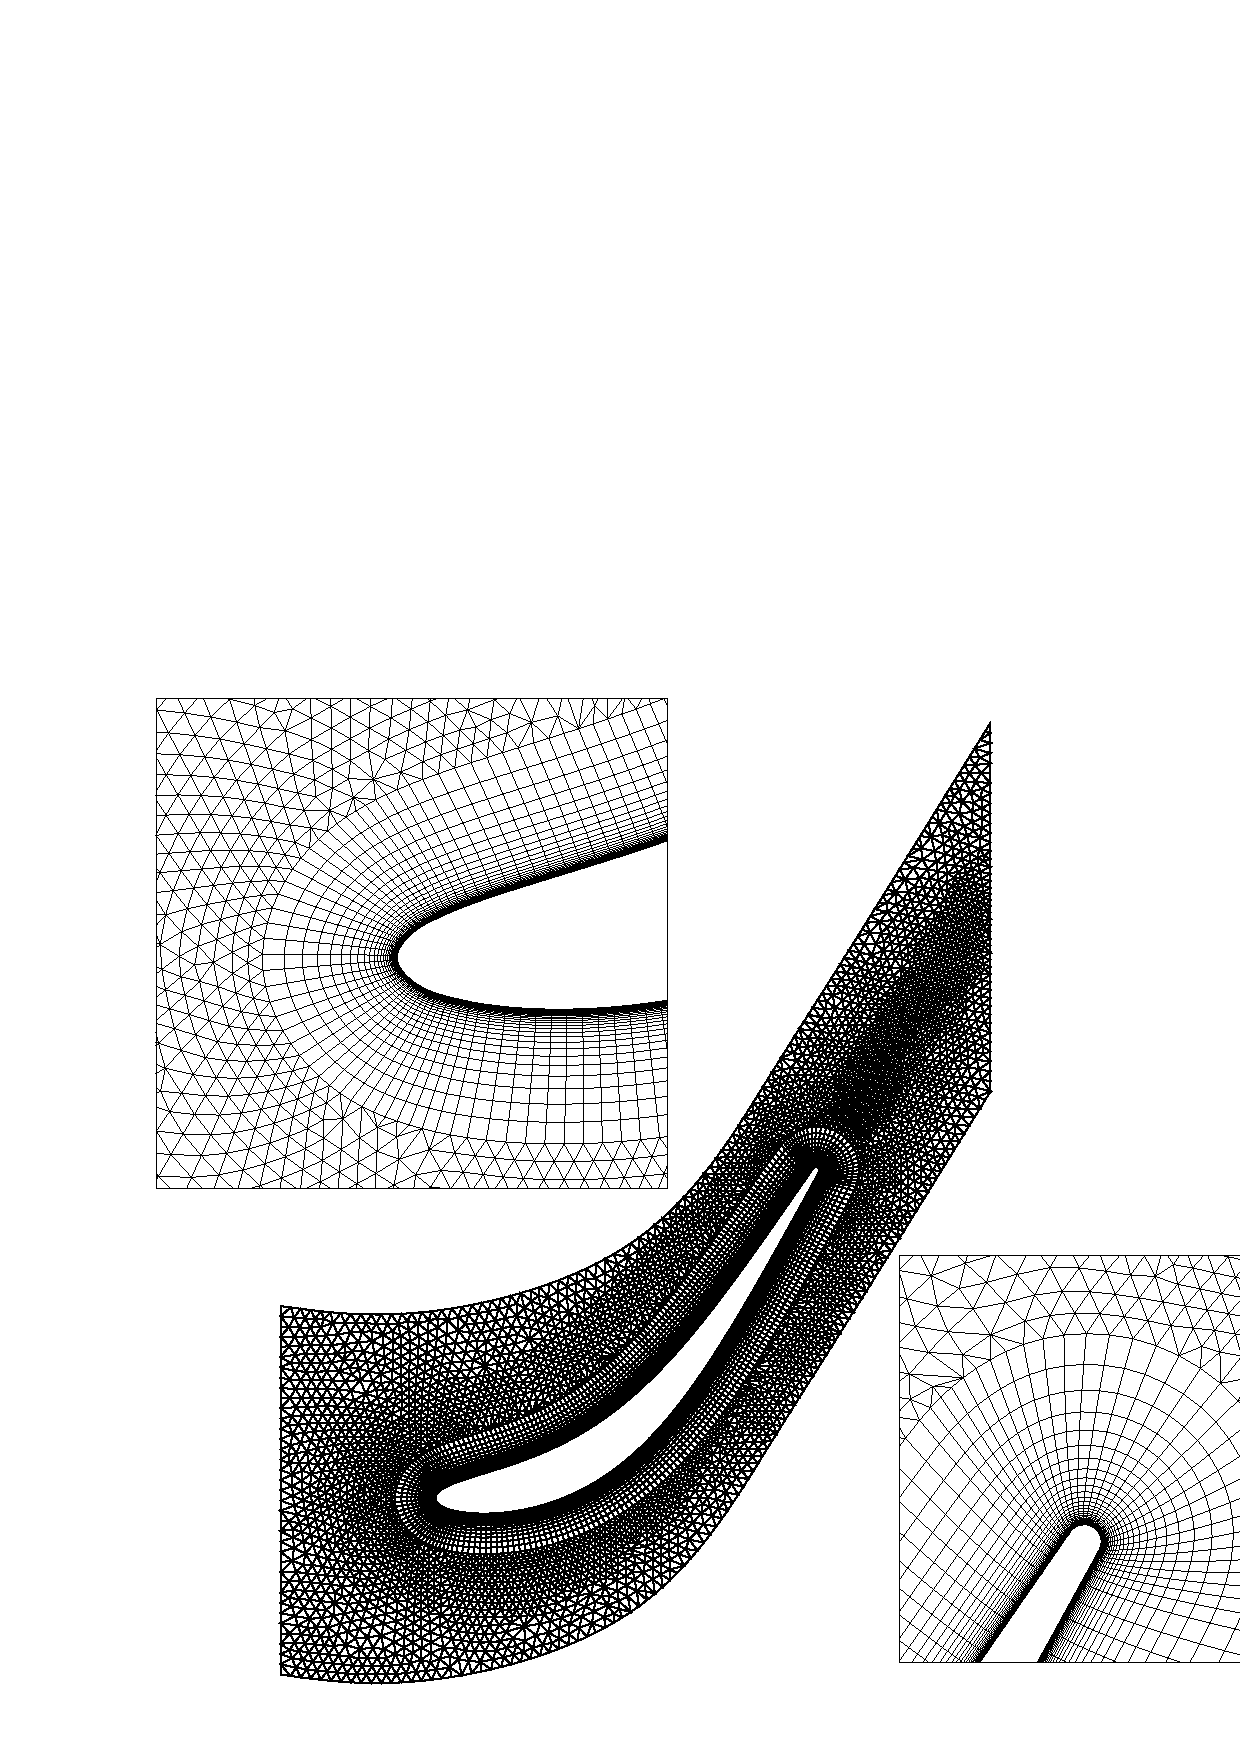
\includegraphics[width=120mm,clip=t]{CHAP_LINEAR/FIGURE/mesh_11th.pdf}}
 \caption{$11^{th}$ Standard configuration. Viscous mesh}
 \label{mesh_11th.fig}
\end{figure}
%
 In this Section the steady and unsteady flow due to bending motion
 of a turbine blade in the direction normal to its chord is analysed.
 The turbine blade geometry under consideration represents the
 $11\se{th}$ International Standard Configuration which have been
 studied for several flow regimes by Fransson et al.
 \citeyear{Bolcs:2}\footnote{The data for the International Standard Configurations
 can be found at {\bf http://www.egi.kth.se/ekv/stcf/} }.
 Two particular flows  will be considered here:
 a subsonic attached flow  and a transonic flow showing a separation
 bubble on the suction surface.
 Fig. \ref{mesh_11th.fig} shows the computational mesh used for all viscous
 calculations. There are 9,312 quadrilaterals in the
 boundary layer region and 7,751 triangles in the rest of the domain, the total  number
 of points being 13,481. A second mesh, used for the inviscid calculations, has
 been obtained from the viscous mesh of Fig. \ref{mesh_11th.fig} by simply removing
 the quadrilateral elements in the boundary layer.

\paragraph{Steady-state flow results.}
%
%
\begin{figure}
 \centerline{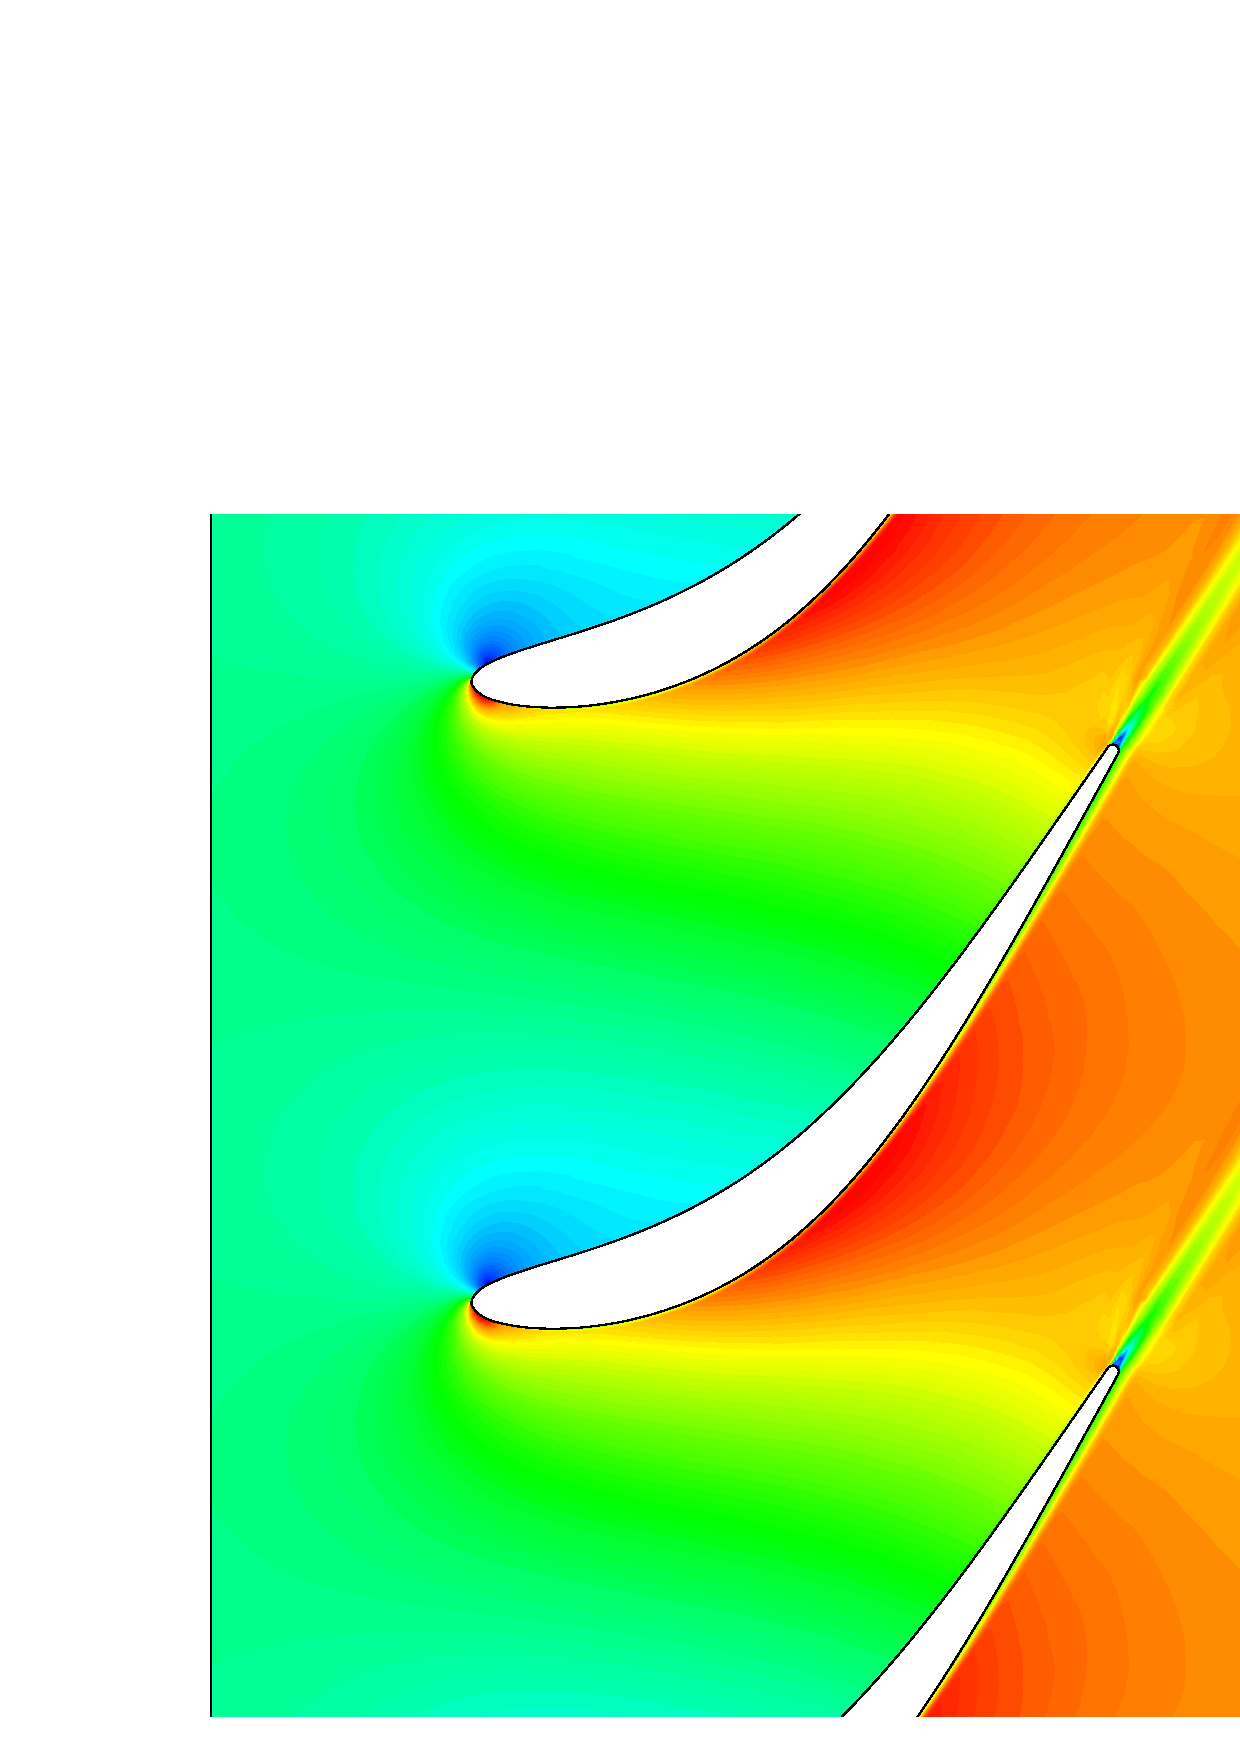
\includegraphics[width=100mm,clip=t]{CHAP_LINEAR/FIGURE/steady_11th_m069_mac_con.pdf}}
 \caption{$11^{th}$ Standard configuration - subsonic case. Steady-state Mach contours}
 \label{conf11_mac_con_069.fig}
\end{figure}
%
%
%
\begin{figure}[ht]
 \centerline{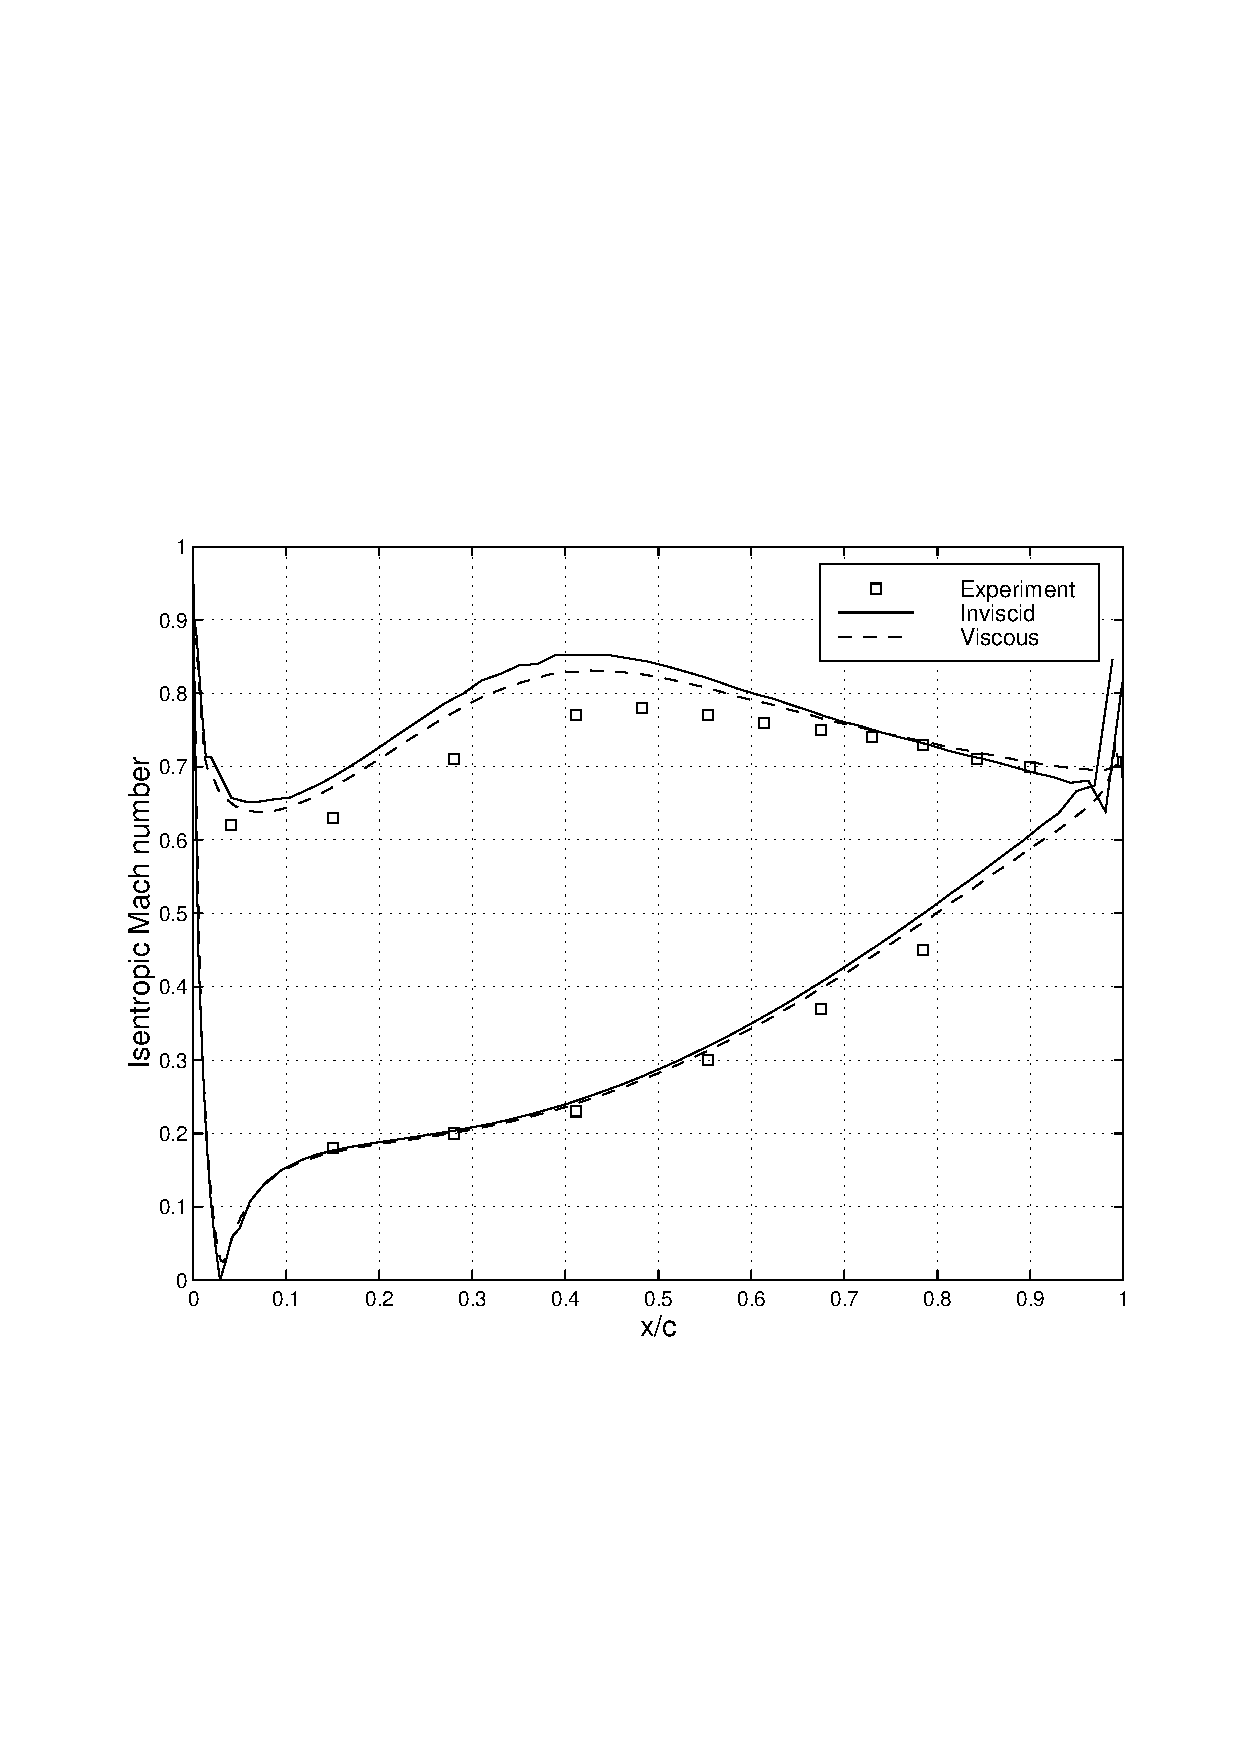
\includegraphics[width=130mm,clip=t]{CHAP_LINEAR/FIGURE/steady_11th_m069_mac_bla.pdf}}
 \caption{$11^{th}$ Standard configuration - subsonic case.
           Isentropic Mach number distribution on the blade}
 \label{conf11_mac_bla_069.fig}
\end{figure}
%
 For the subsonic flow case the inlet flow angle is $-15.2\se{o}$,
 the outlet isentropic Mach number is 0.69
 and the inlet Reynolds number, based on the blade's chord, is $650,000$.
 The maximum value of $y+$ is of around 4 which guarantees a good resolution of the
 viscous sublayer using the Spalart-Allmaras turbulence model.
 The predicted Mach number contours are shown in Fig. \ref{conf11_mac_con_069.fig}
 while a comparison of the inviscid and viscous analyses with measured data is given in
 Fig. \ref{conf11_mac_bla_069.fig}.
 For the suction surface, both the viscous and inviscid computations somewhat
 overpredict the Mach number distribution at around mid-chord. However, a similar
 solution was obtained by  Fransson et al. \citeyear{Bolcs:2} and the reasons for
 the discrepancy are discussed in some detail. Here, we will consider that the
 steady-state flow has been captured adequately for the purposes of providing a
 starting point for the linearised unsteady flow.

 For the transonic off-design case the inlet flow angle is $34\se{o}$,
 the outlet isentropic Mach number is $1$ and the inlet Reynolds number,
 based on the blade's chord, is $860,000$. The maximum $y+$ value is around 5.
 The predicted Mach number contours are plotted in Fig. \ref{conf11_mac_con_099.fig}a.
 A particular feature of the flow, the recirculation bubble on the suction
 surface, is shown in Fig. \ref{conf11_mac_con_099.fig}b.
 Because of the significant viscous features,
 the Navier-Stokes analysis shows a much better agreement
 with the measured data, with perhaps the exception of the trailing-edge behaviour
 (Fig. \ref{conf11_mac_bla_099.fig}).
 However, as discussed by Fransson et al. \citeyear{Bolcs:2}, the pre-shock
 Mach number is very sensitive to the experimental inlet conditions.
 In any case, as expected, a viscous
 analysis is required to predict  the separation bubble of the suction side which
 occurs between $10-30\%$  blade chord, a feature that can be seen from  the flow
 deceleration in Fig. \ref{conf11_mac_bla_099.fig}. As will be discussed below,
 such differences in the steady-state flow will lead to major
 discrepancies for unsteady flow predictions.
%
\begin{figure}[ht]
 \begin{center}
  \begin{tabular}{c}
    \subfigure[Mach contours]
       {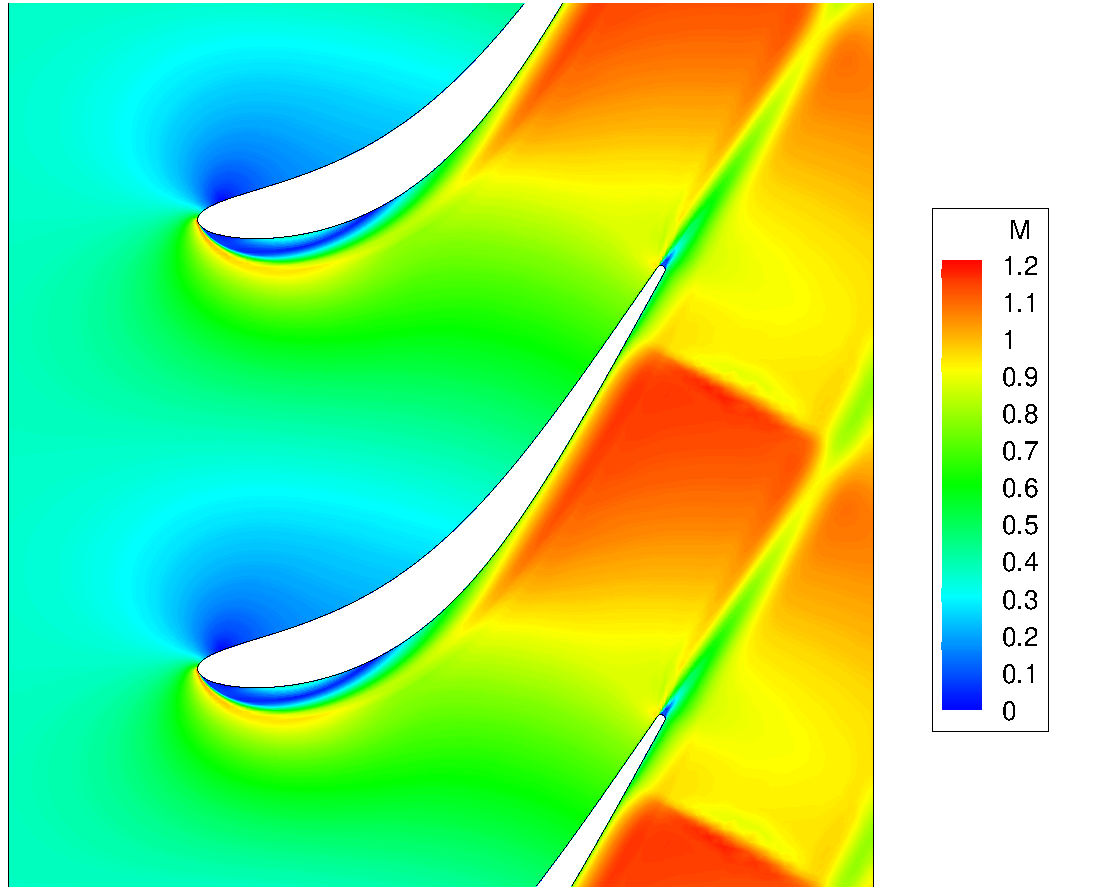
\includegraphics[width=80mm,clip=t]{CHAP_LINEAR/FIGURE/steady_11th_m099_mac_con.pdf}}\\
    \subfigure[Particle traces in the separation bubble]
       {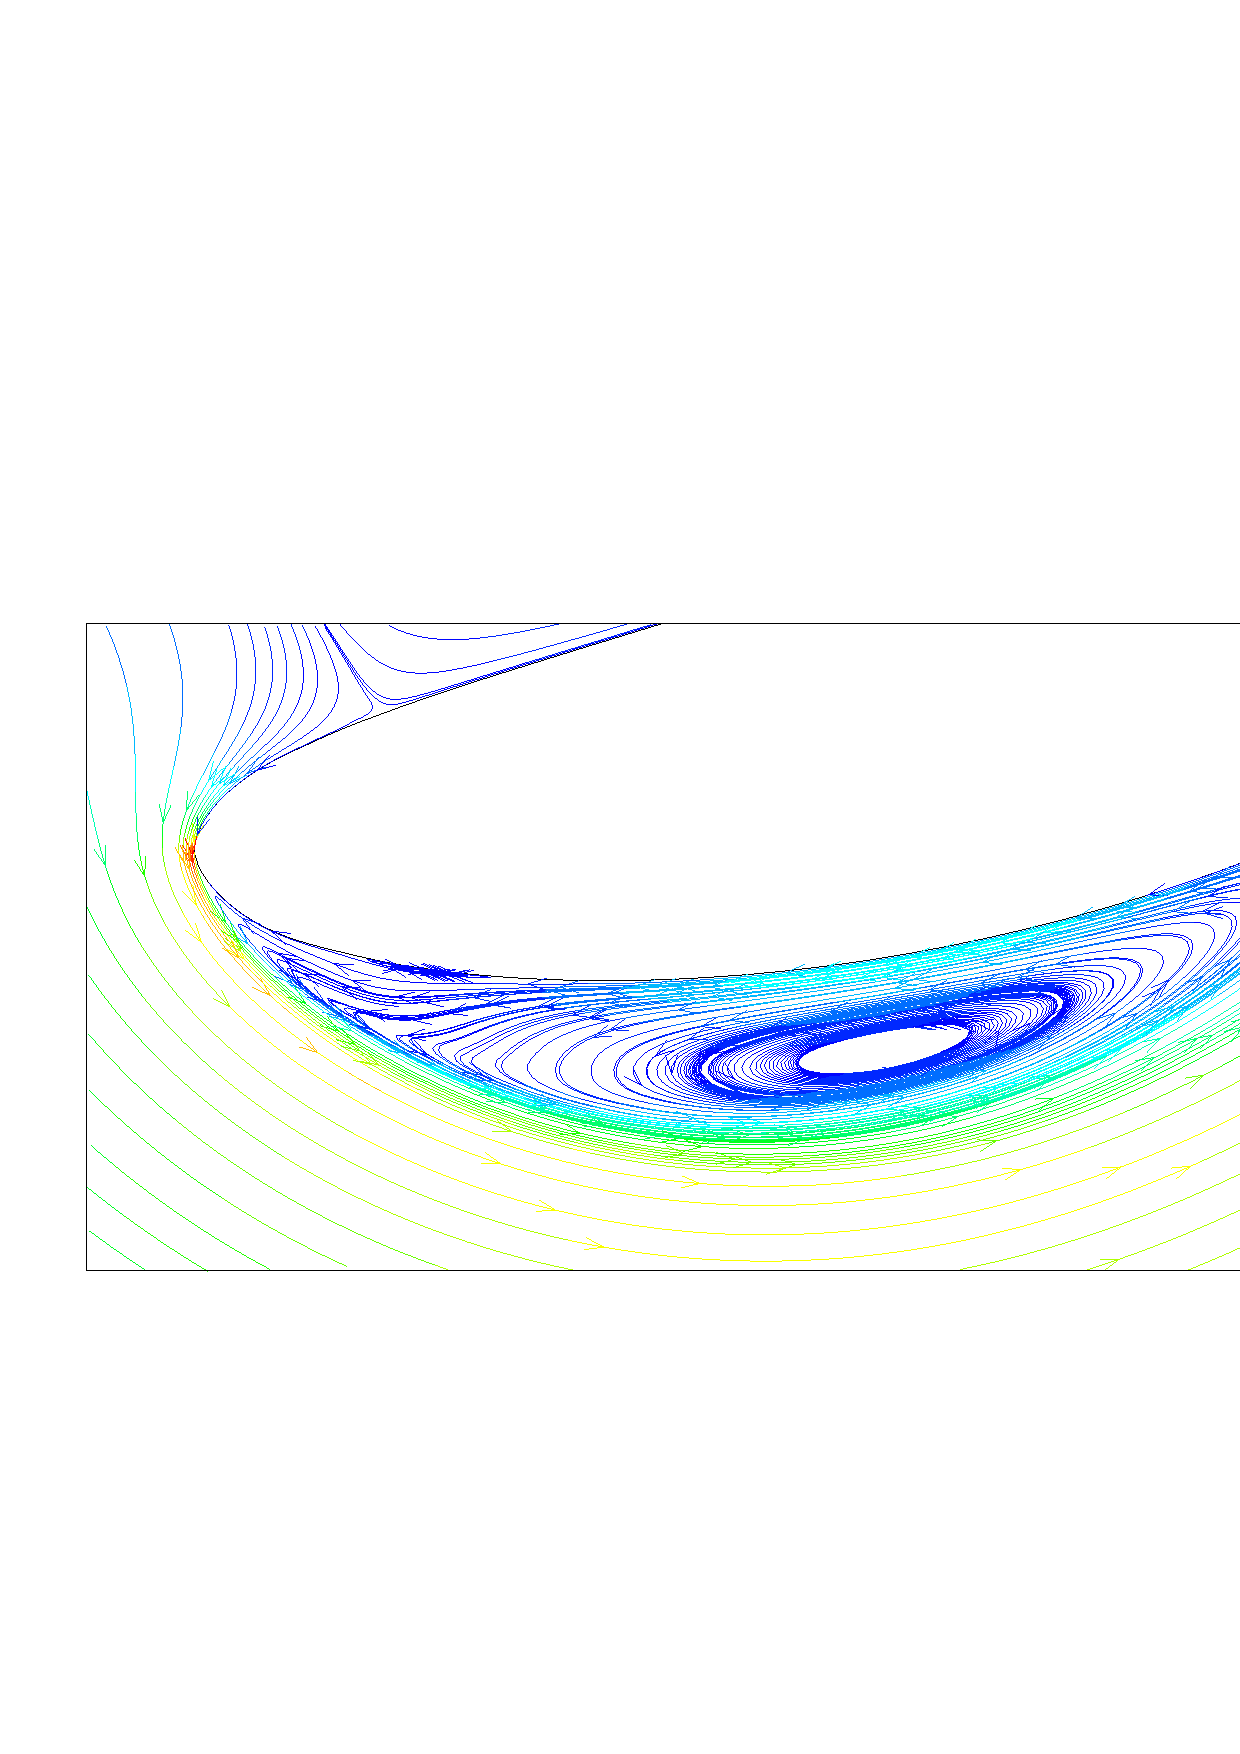
\includegraphics[width=80mm,clip=t]{CHAP_LINEAR/FIGURE/steady_11th_m099_stream.pdf}}
  \end{tabular}
 \end{center}
 \vspace{-7mm}
 \caption{$11^{th}$ Standard configuration - transonic case. Steady-state Mach contours}
 \label{conf11_mac_con_099.fig}
\end{figure}
%
%
\begin{figure}[ht]
 \centerline{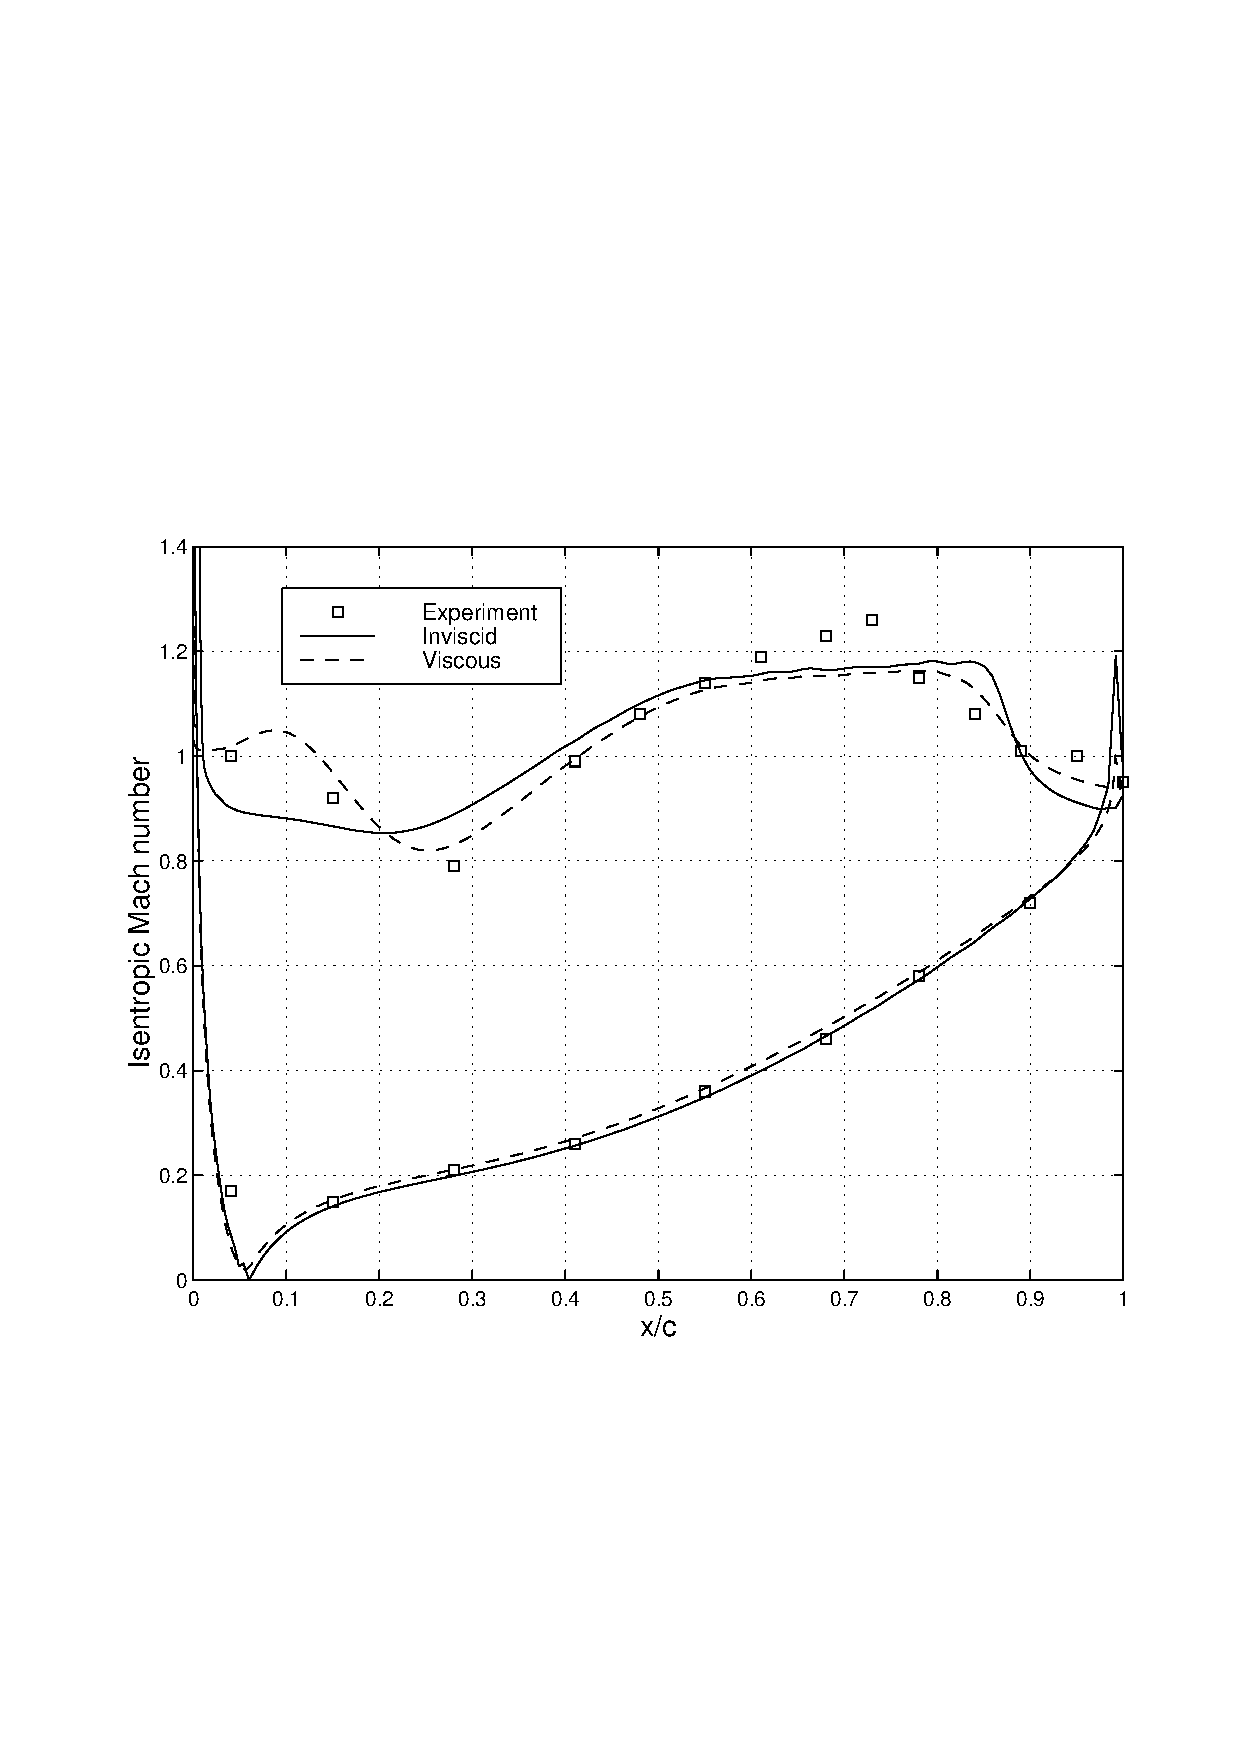
\includegraphics[width=130mm,clip=t]{CHAP_LINEAR/FIGURE/steady_11th_m099_mac_bla.pdf}}
 \caption{$11^{th}$ Standard configuration - transonic case.
           Isentropic Mach number distribution on the blade}
 \label{conf11_mac_bla_099.fig}
\end{figure}
%
%
%
\paragraph{Linearised unsteady flow results}
 The unsteadiness  due to bending motion
 of the blade in the direction normal to its chord was computed using the linearised
 flow solver. The  reduced frequency is 0.21 for the
 subsonic case and 0.15 for the transonic case.  Three different sets of flow calculations were
 performed for each case:  (i) inviscid linearised using an inviscid base steady-state flow,
 (ii) viscous linearised with frozen turbulence using viscous fully-turbulent
 base flow, and (iii) viscous fully-linearised  using the same viscous
 base flow as in (ii).
 In calculations (ii), neither the laminar nor the turbulent
 viscosities were linearised and their values were kept fixed at their steady-state values.
 Calculations (iii) were performed with a fully-linearised Spalart-Allmaras turbulence
 model.

 The amplitude and phase of the predicted unsteady
 pressure coefficient\footnote{$\widetilde{c}\sm{p} =
 \frac{c\, \widetilde{p}}{h\left(p\sm{01} - p\sm{1}\right)}$, where $h$ is the
 bending amplitude and $c$ the blade chord.}
 distribution are compared to measured data in Figs.
 \ref{subsonic_11_ampl.fig} and \ref{subsonic_11_phas.fig} for the subsonic case.
 The first noticeable feature is the similarity of the amplitude predictions for the
 three modelling levels, though some deviations can be observed for the phase plots.
 This result is somewhat expected because of the similarity of the inviscid and
 viscous steady-state solutions.
 There is reasonable overall agreement with the measured data, though the undershoot
 at around $50\%$ chord is not captured in any of the computations.
 An inspection of the phase plots reveals that the negative to positive
 (or stable to unstable)  phase jump, is predicted
 much further downstream than the measured position.
 However, the fully non-linear viscous unsteady calculations of Franson et al.
 \citeyear{Bolcs:2} exhibit the same trend and hence the cause of the discrepancy
 is not due to linearisation.

 The amplitude and phase of the predicted unsteady
 pressure distribution is compared to measured data
 in Figs. \ref{transonic_11_ampl.fig} and \ref{transonic_11_phas.fig}
 for the transonic case.
 The discrepancies between different the three modelling levels is now more pronounced.
 The linearised inviscid approach is seen to overpredict the unsteady
 pressure coefficient on the suction side of the blade both in the recirculation
 region ($0 - 30\%$ of chord) and around the trailing-edge.  In the recirculation region,
 the full linearisation of the viscous terms yields better results than freezing
 the turbulence model and the two approaches are seen to be equivalent elsewhere.
%
%
\begin{figure}
 \begin{center}
  \begin{tabular}{c}
    {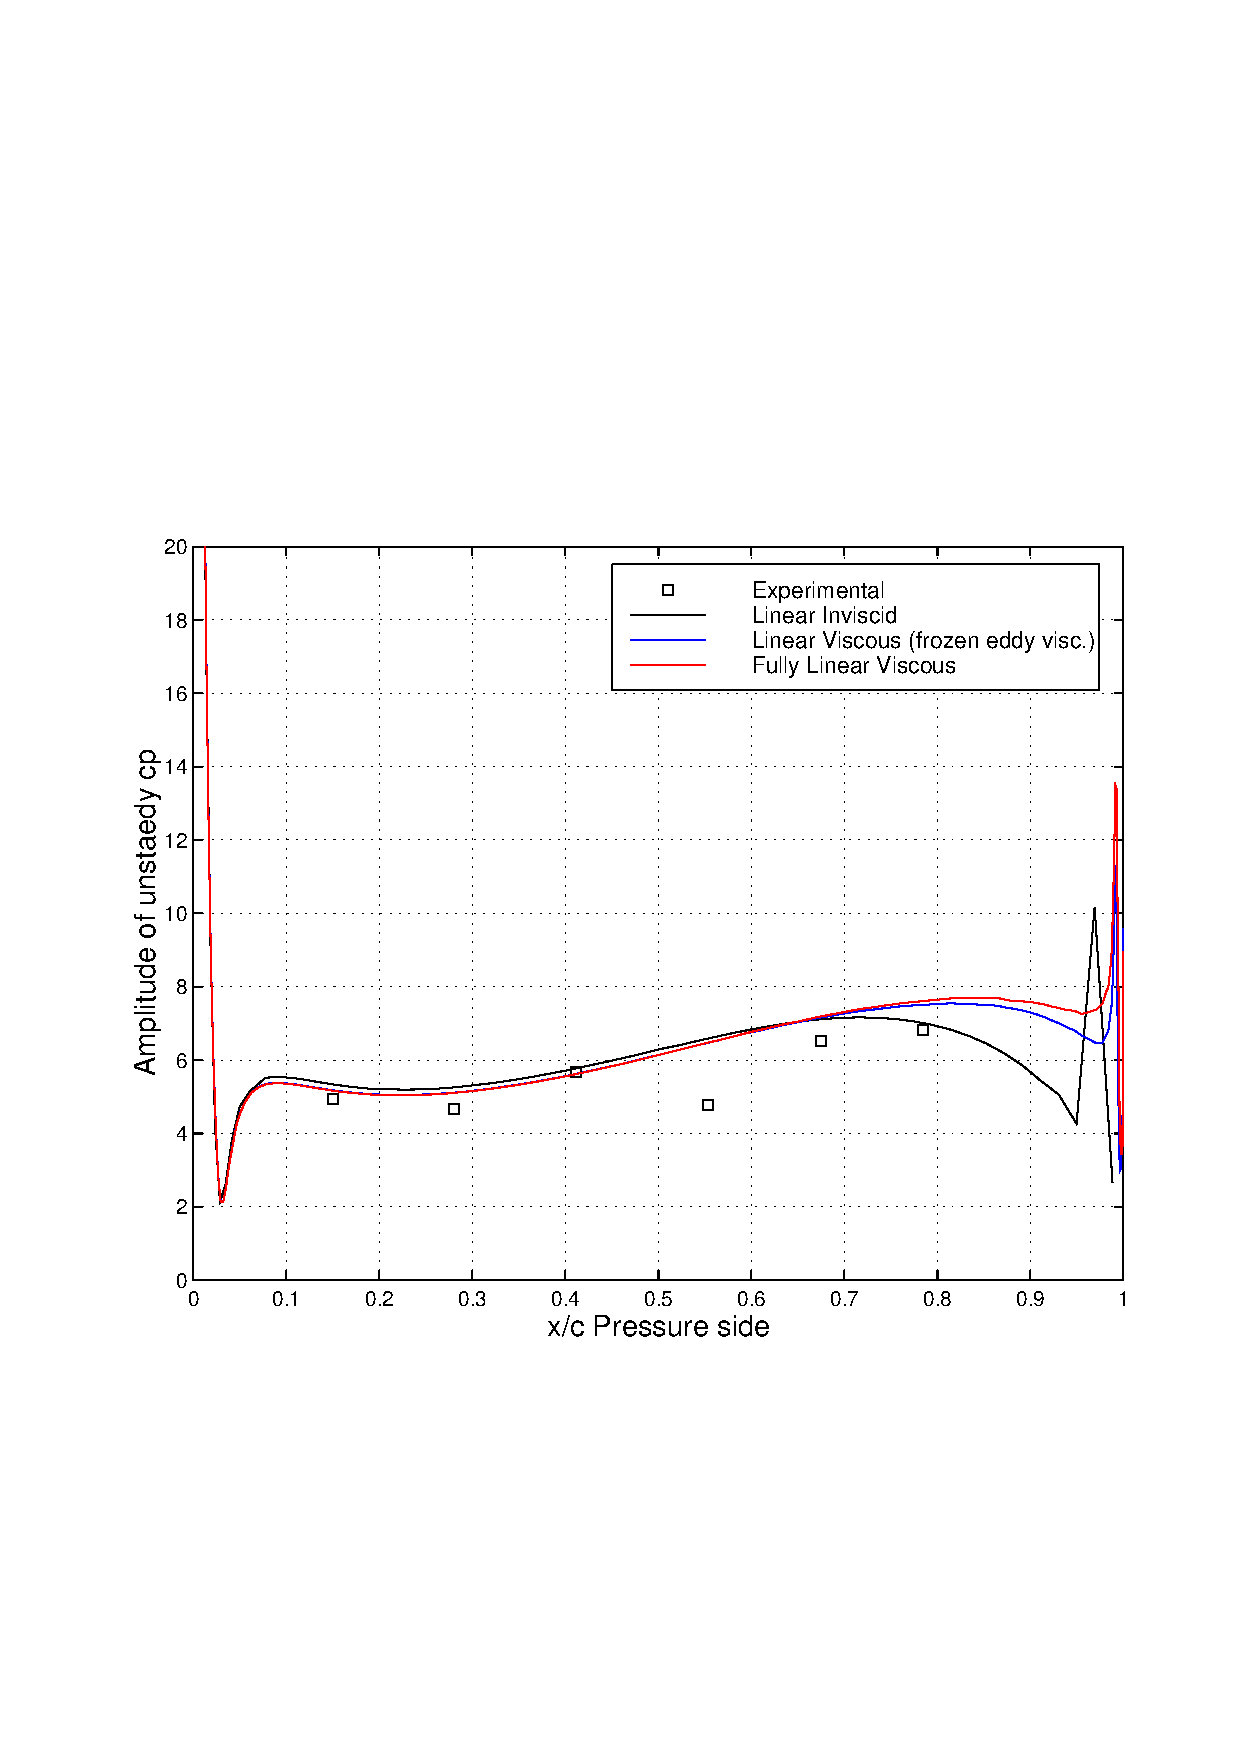
\includegraphics[height=100mm,clip=t]{CHAP_LINEAR/FIGURE/unsteady_blade_069_180_1.pdf}}\\
    {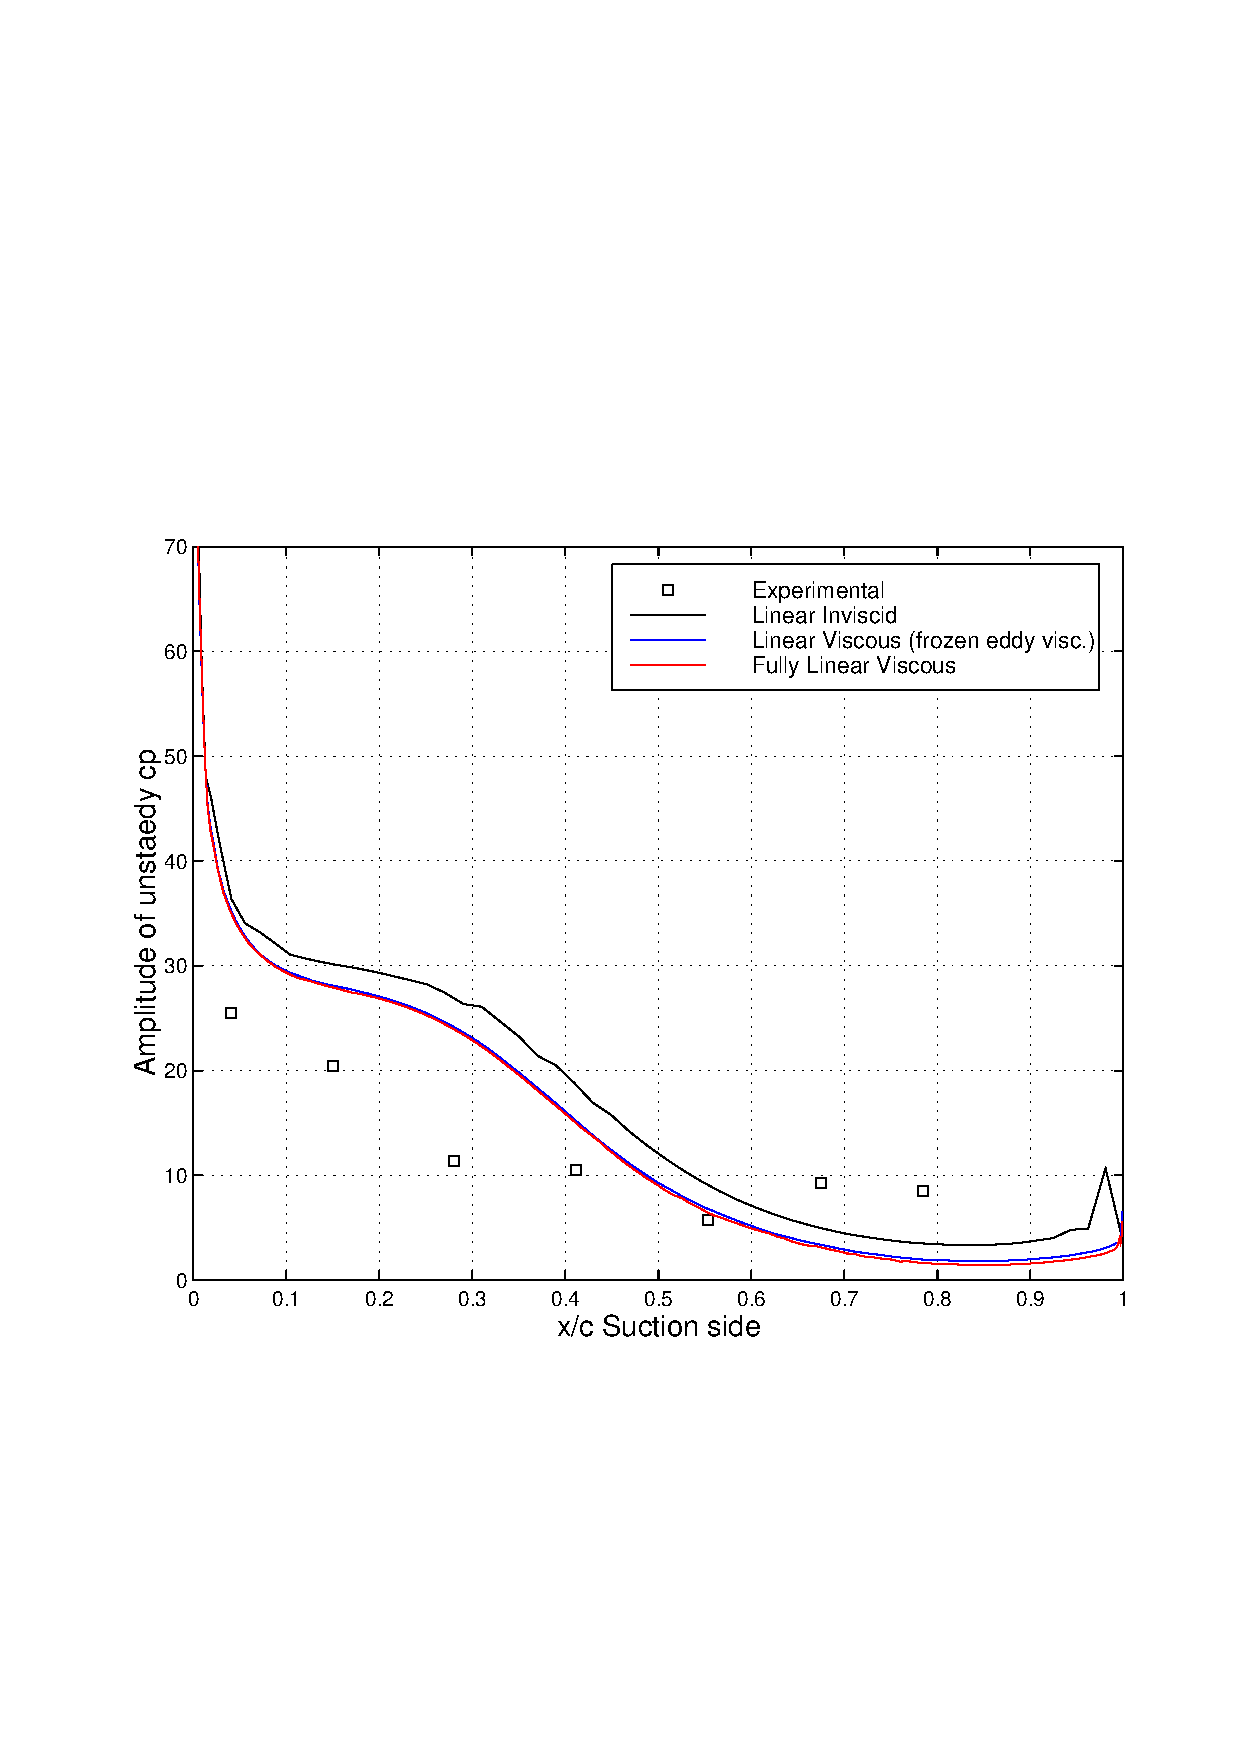
\includegraphics[height=100mm,clip=t]{CHAP_LINEAR/FIGURE/unsteady_blade_069_180_2.pdf}}
  \end{tabular}
 \end{center}
 \vspace{-7mm}
 \caption{$11^{th}$ Standard configuration - subsonic case.
          Amplitude of $\tilde{c}\sm{p}$
         ($\omega = 0.21$, $\phi = 180\se{o}$)}
 \label{subsonic_11_ampl.fig}
\end{figure}
%
\begin{figure}
 \begin{center}
  \begin{tabular}{c}
    {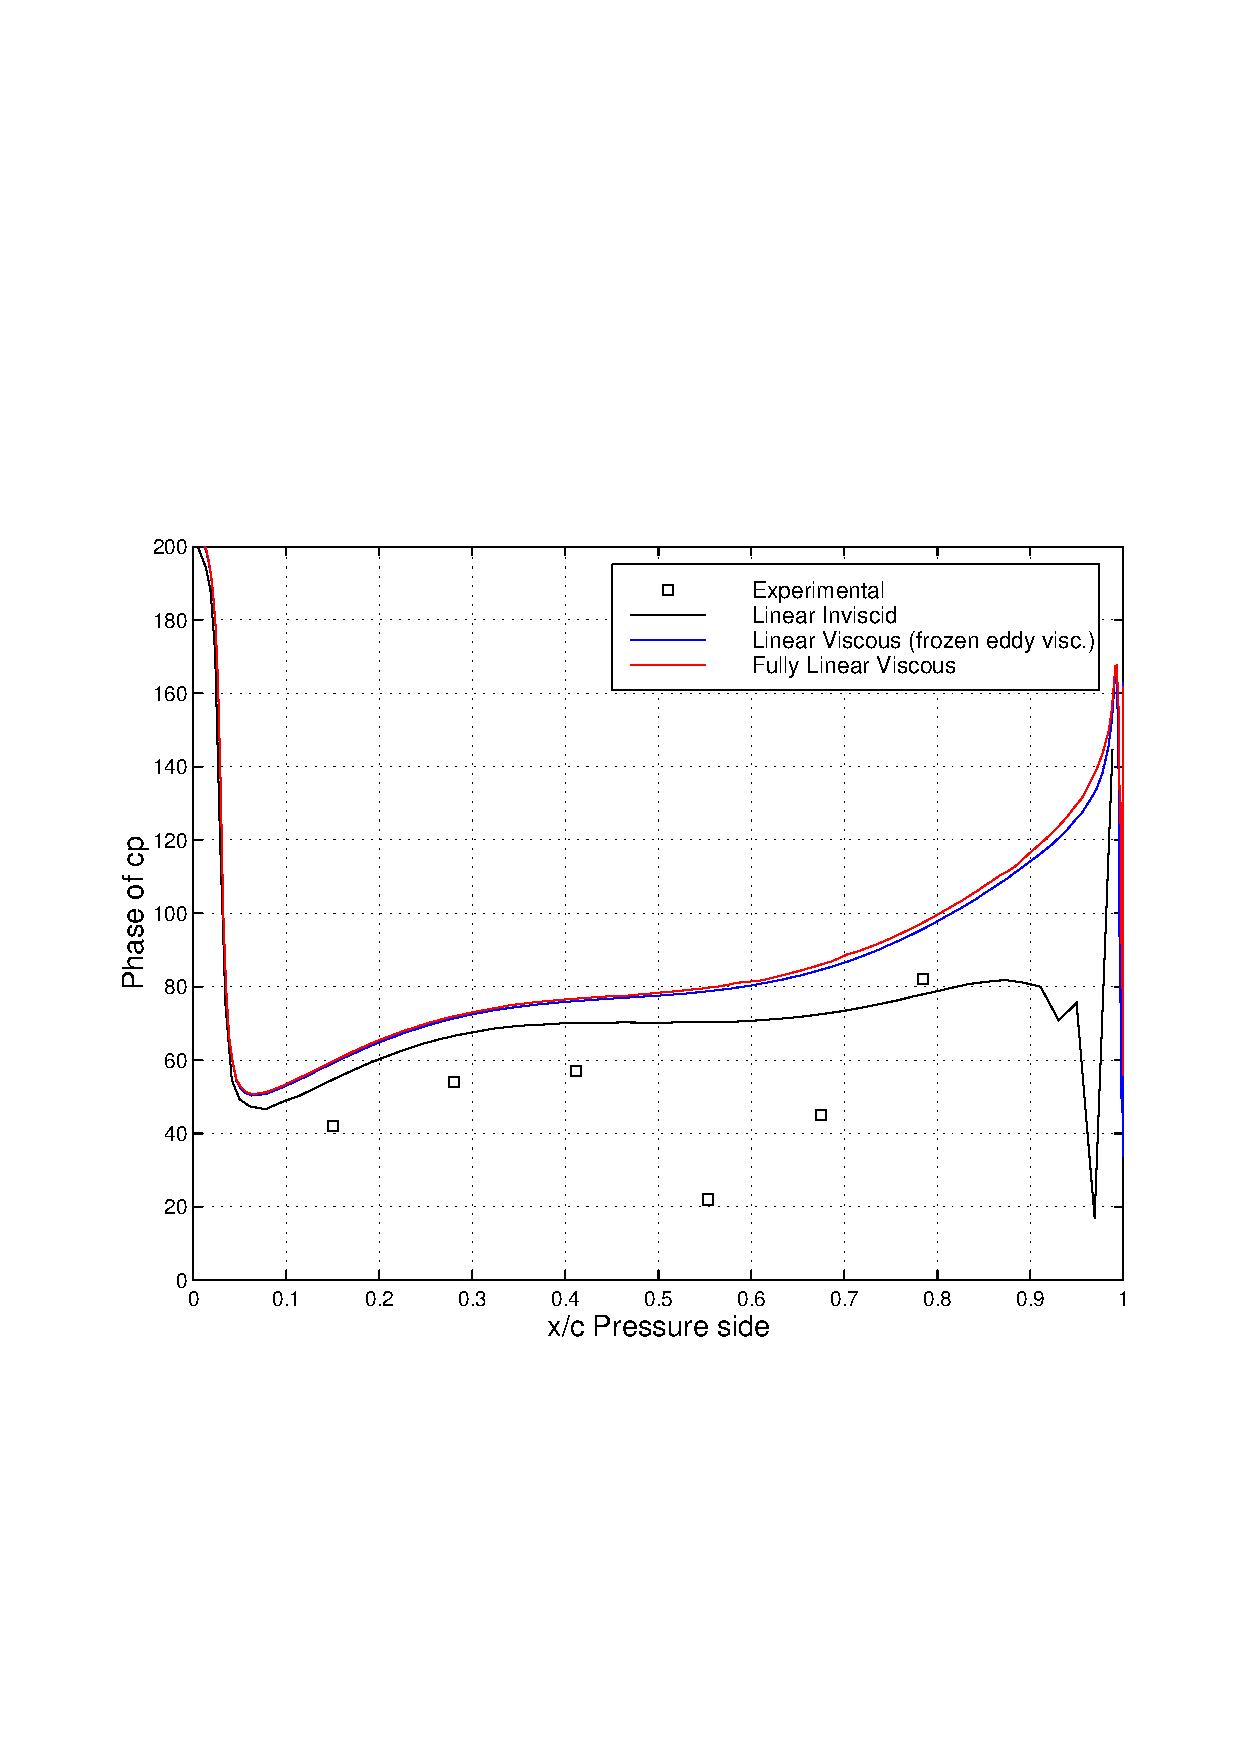
\includegraphics[height=100mm,clip=t]{CHAP_LINEAR/FIGURE/unsteady_blade_069_180_3.pdf}}\\
    {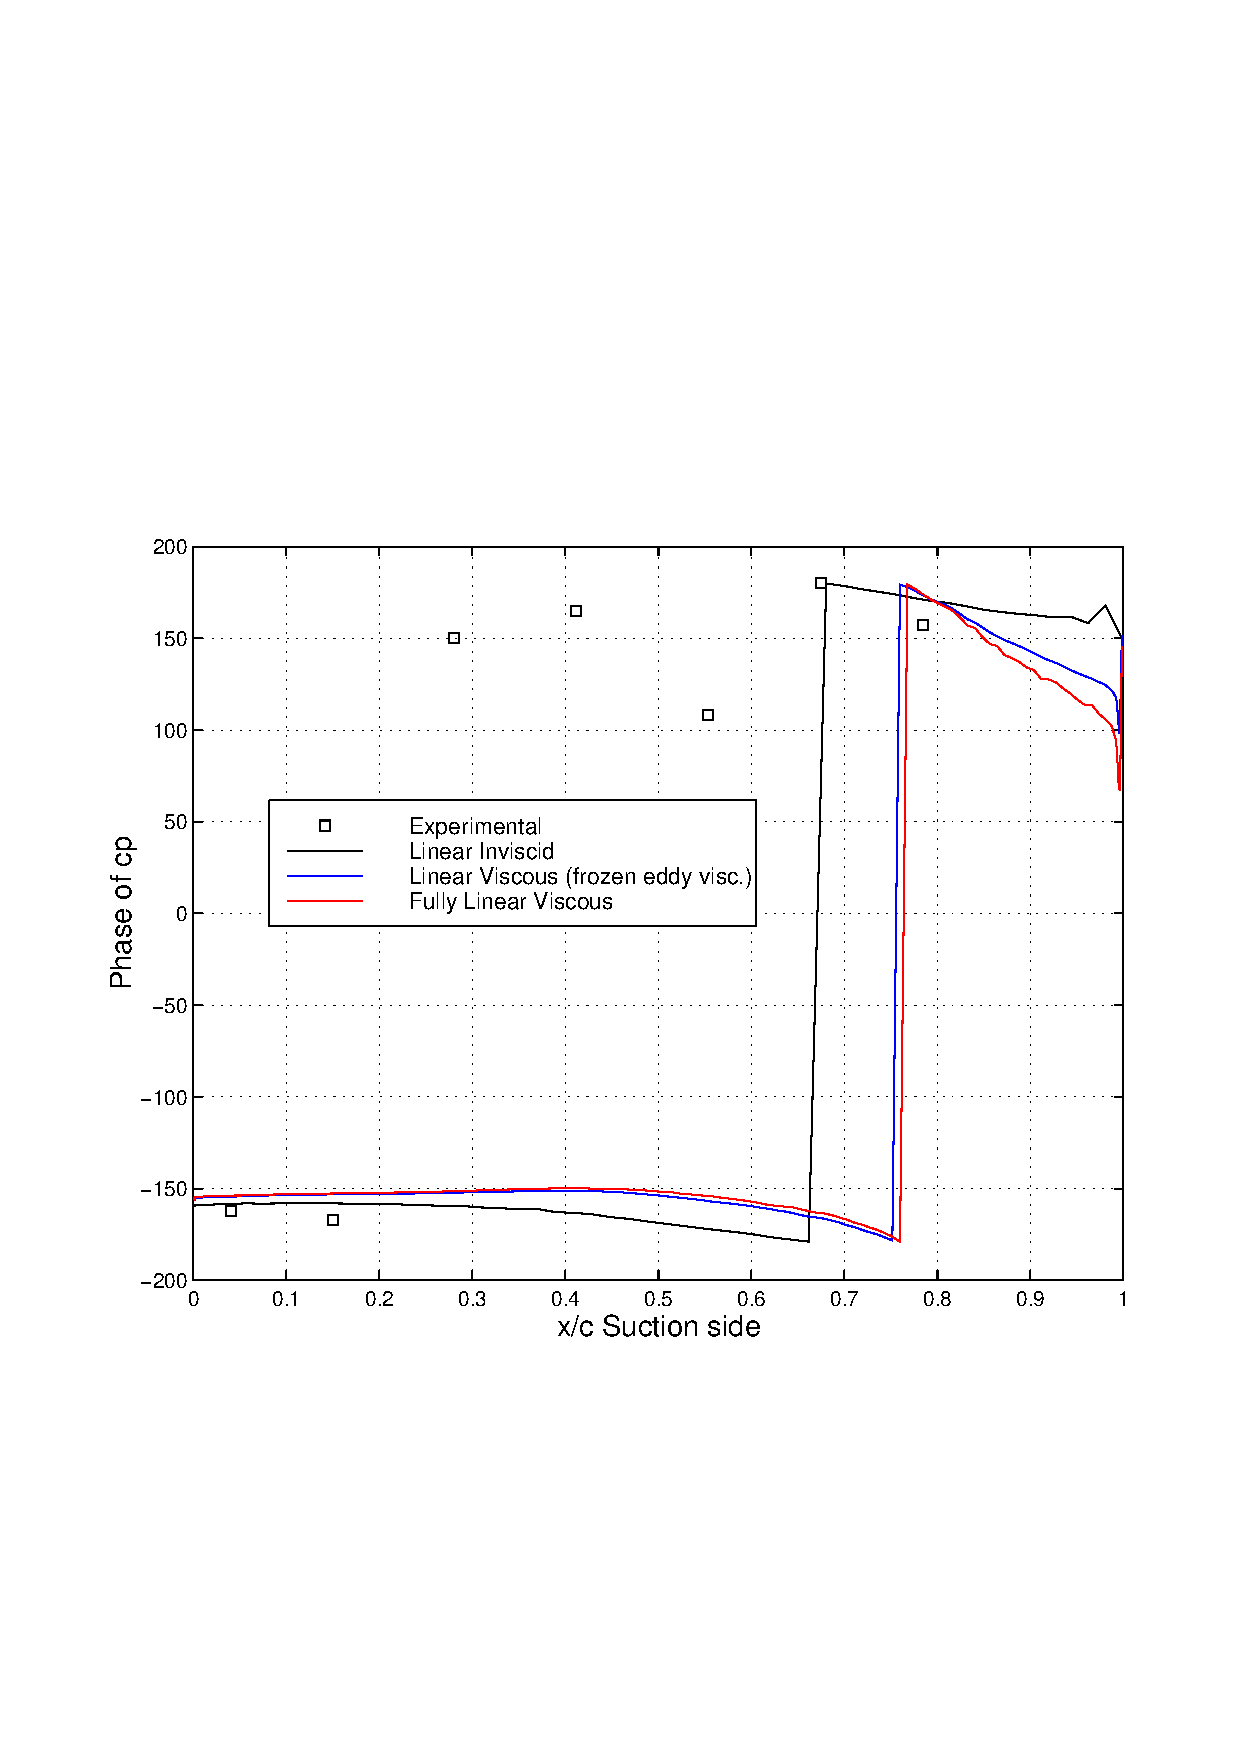
\includegraphics[height=100mm,clip=t]{CHAP_LINEAR/FIGURE/unsteady_blade_069_180_4.pdf}}
  \end{tabular}
 \end{center}
 \vspace{-7mm}
 \caption{$11^{th}$ Standard configuration - subsonic case.
          Phase of of $\tilde{c}\sm{p}$
         ($\omega = 0.21$, $\phi = 180\se{o}$)}
 \label{subsonic_11_phas.fig}
\end{figure}
%
\begin{figure}
 \begin{center}
  \begin{tabular}{c}
    {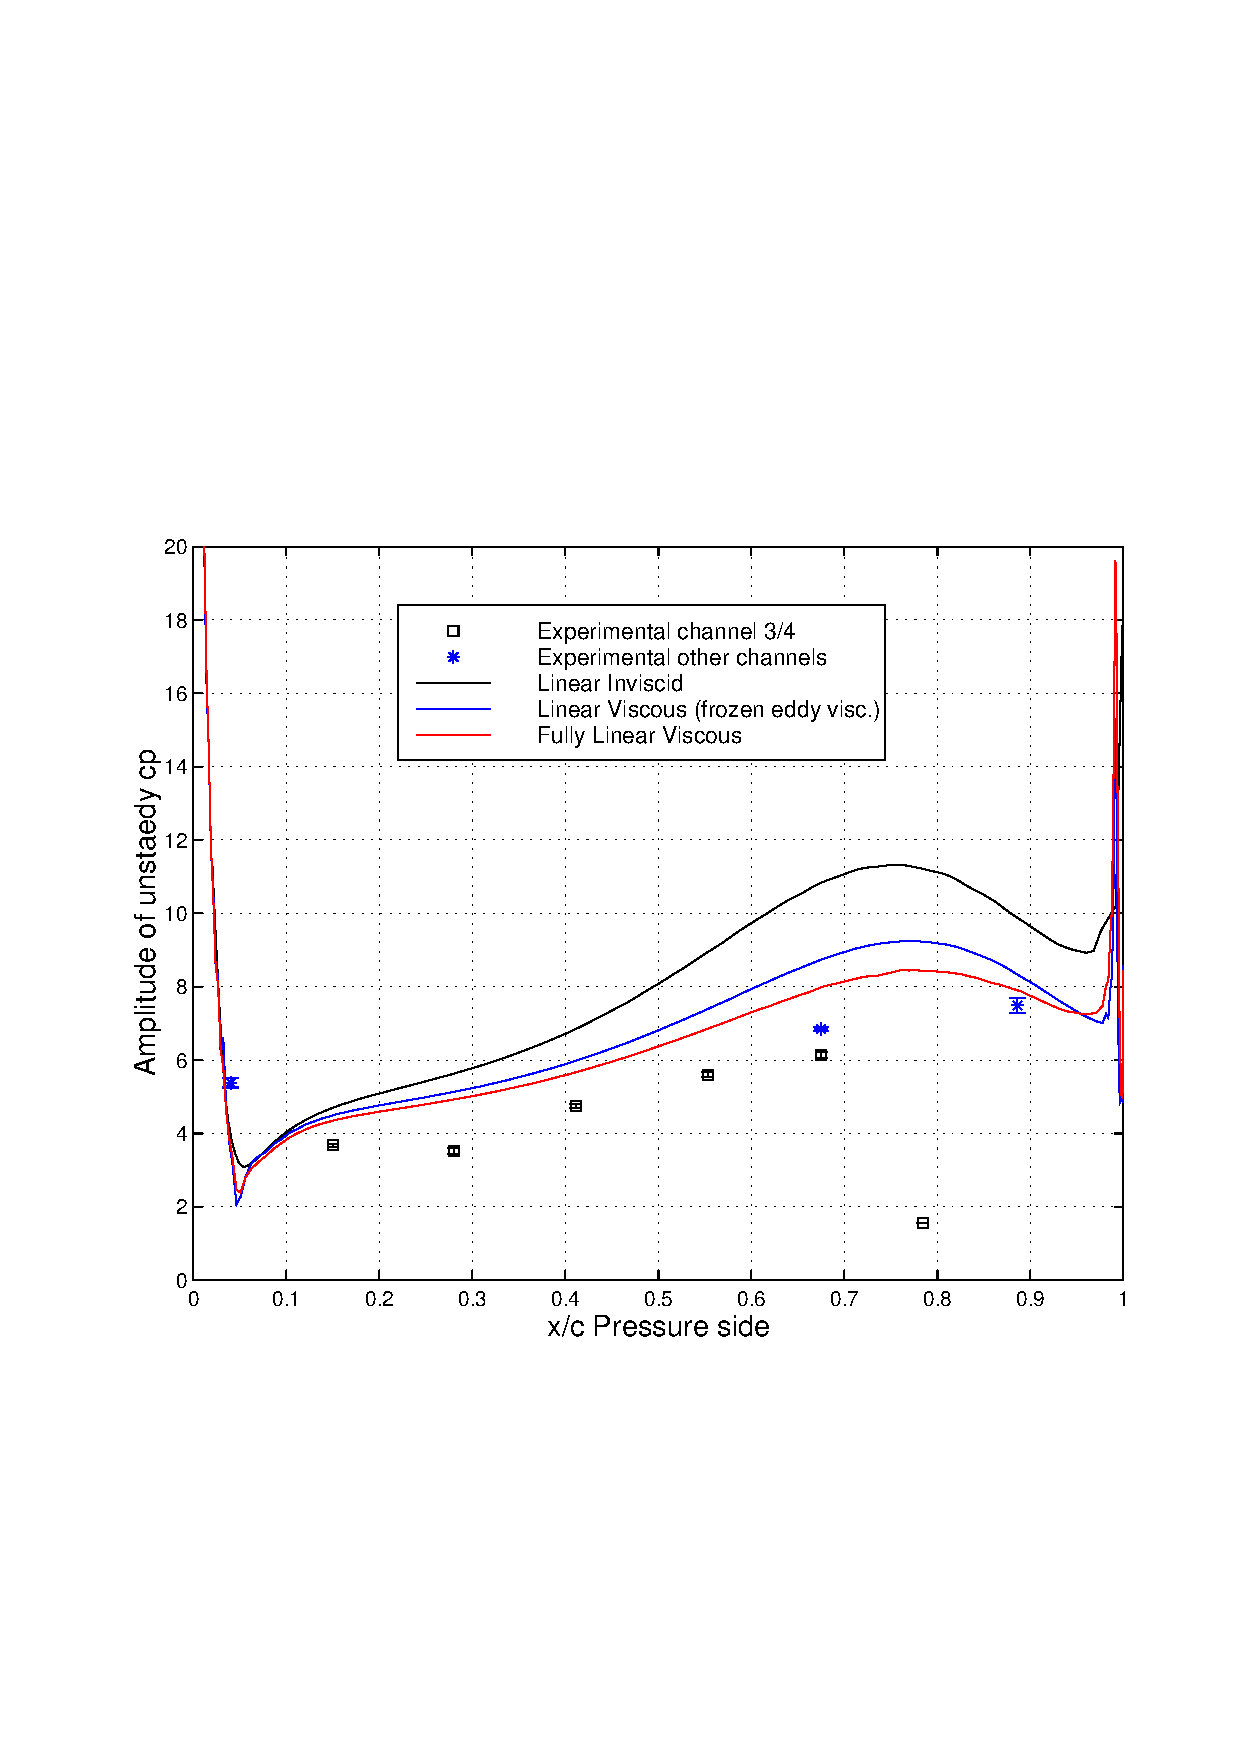
\includegraphics[height=100mm,clip=t]{CHAP_LINEAR/FIGURE/unsteady_blade_099_180_1.pdf}}\\
    {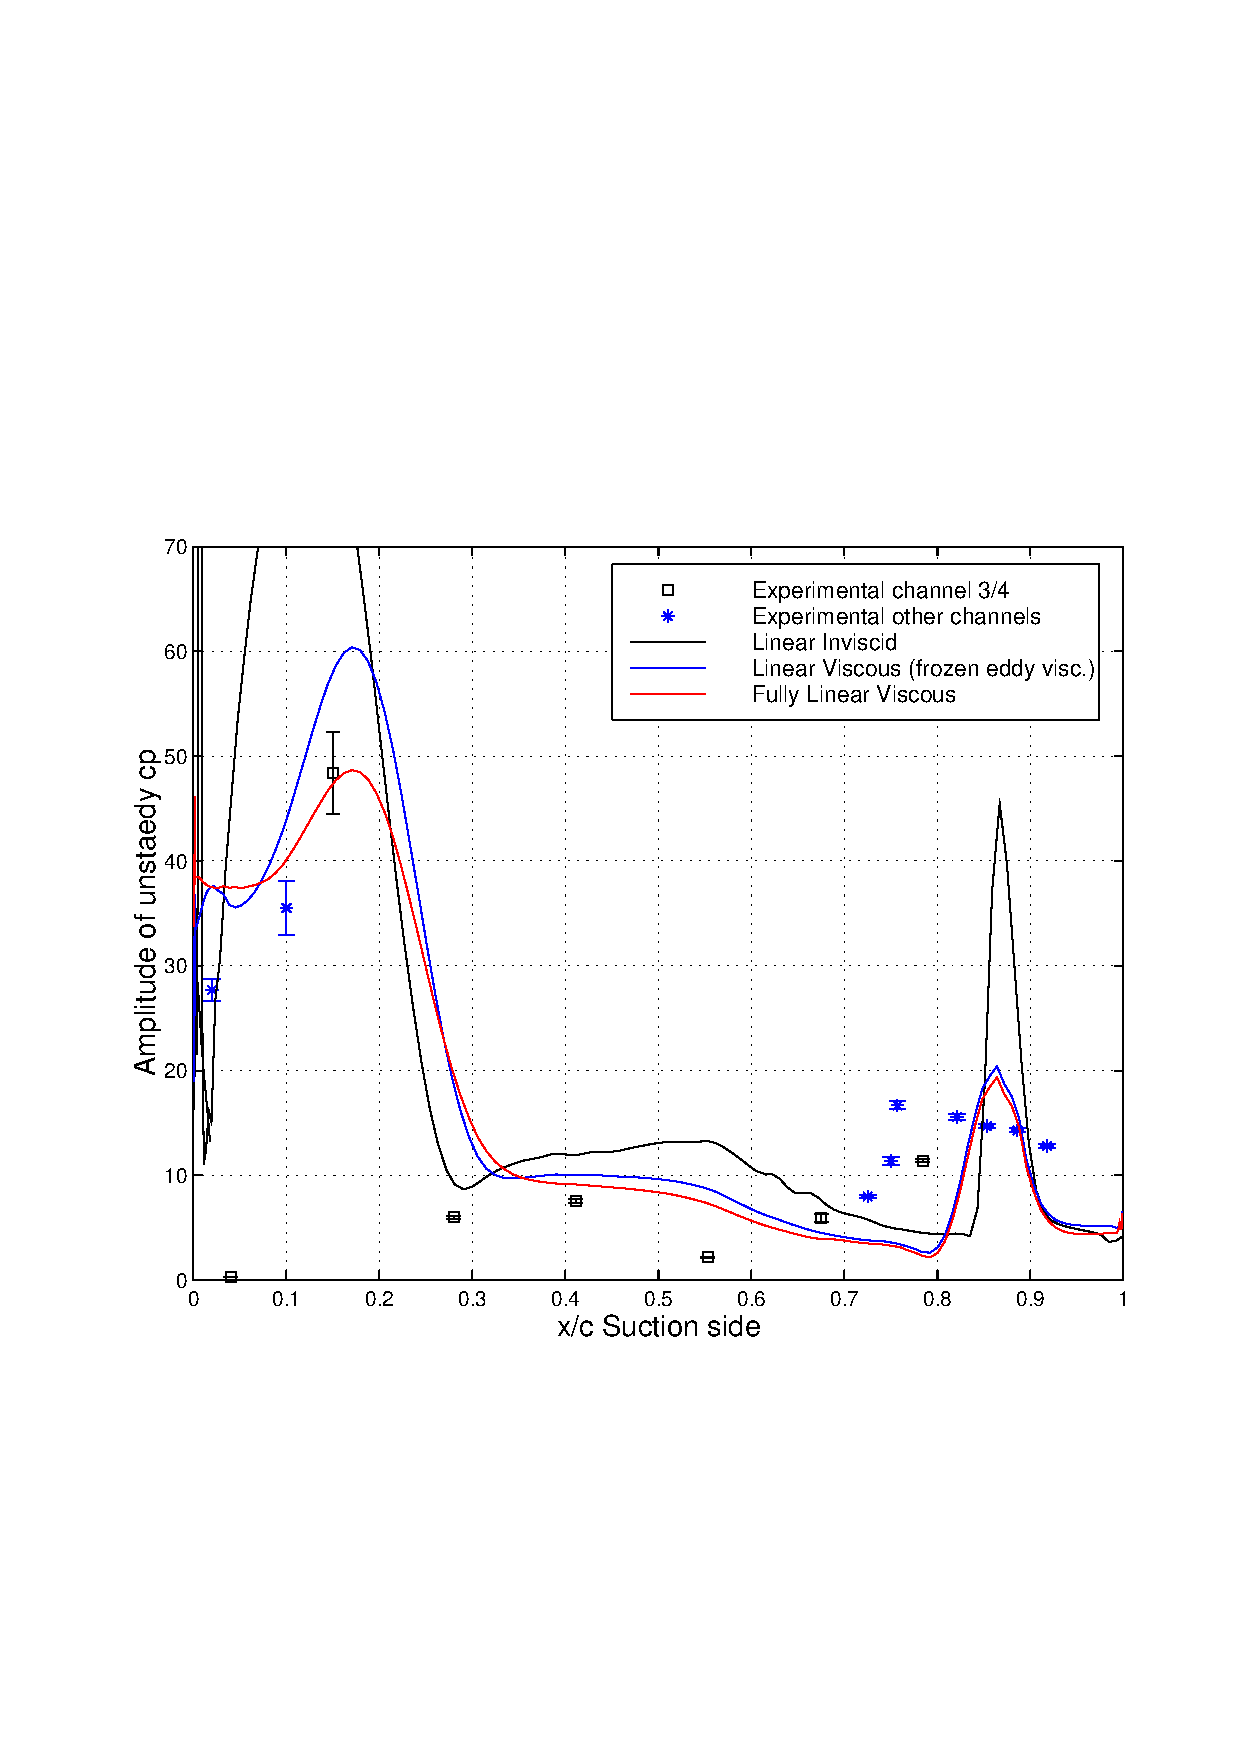
\includegraphics[height=100mm,clip=t]{CHAP_LINEAR/FIGURE/unsteady_blade_099_180_2.pdf}}
  \end{tabular}
 \end{center}
 \vspace{-7mm}
 \caption{$11^{th}$ Standard configuration - transonic case.
          Amplitude of $\tilde{c}\sm{p}$
         ($\omega = 0.15$, $\phi = 180\se{o}$)}
 \label{transonic_11_ampl.fig}
\end{figure}
%
\begin{figure}
 \begin{center}
  \begin{tabular}{c}
    {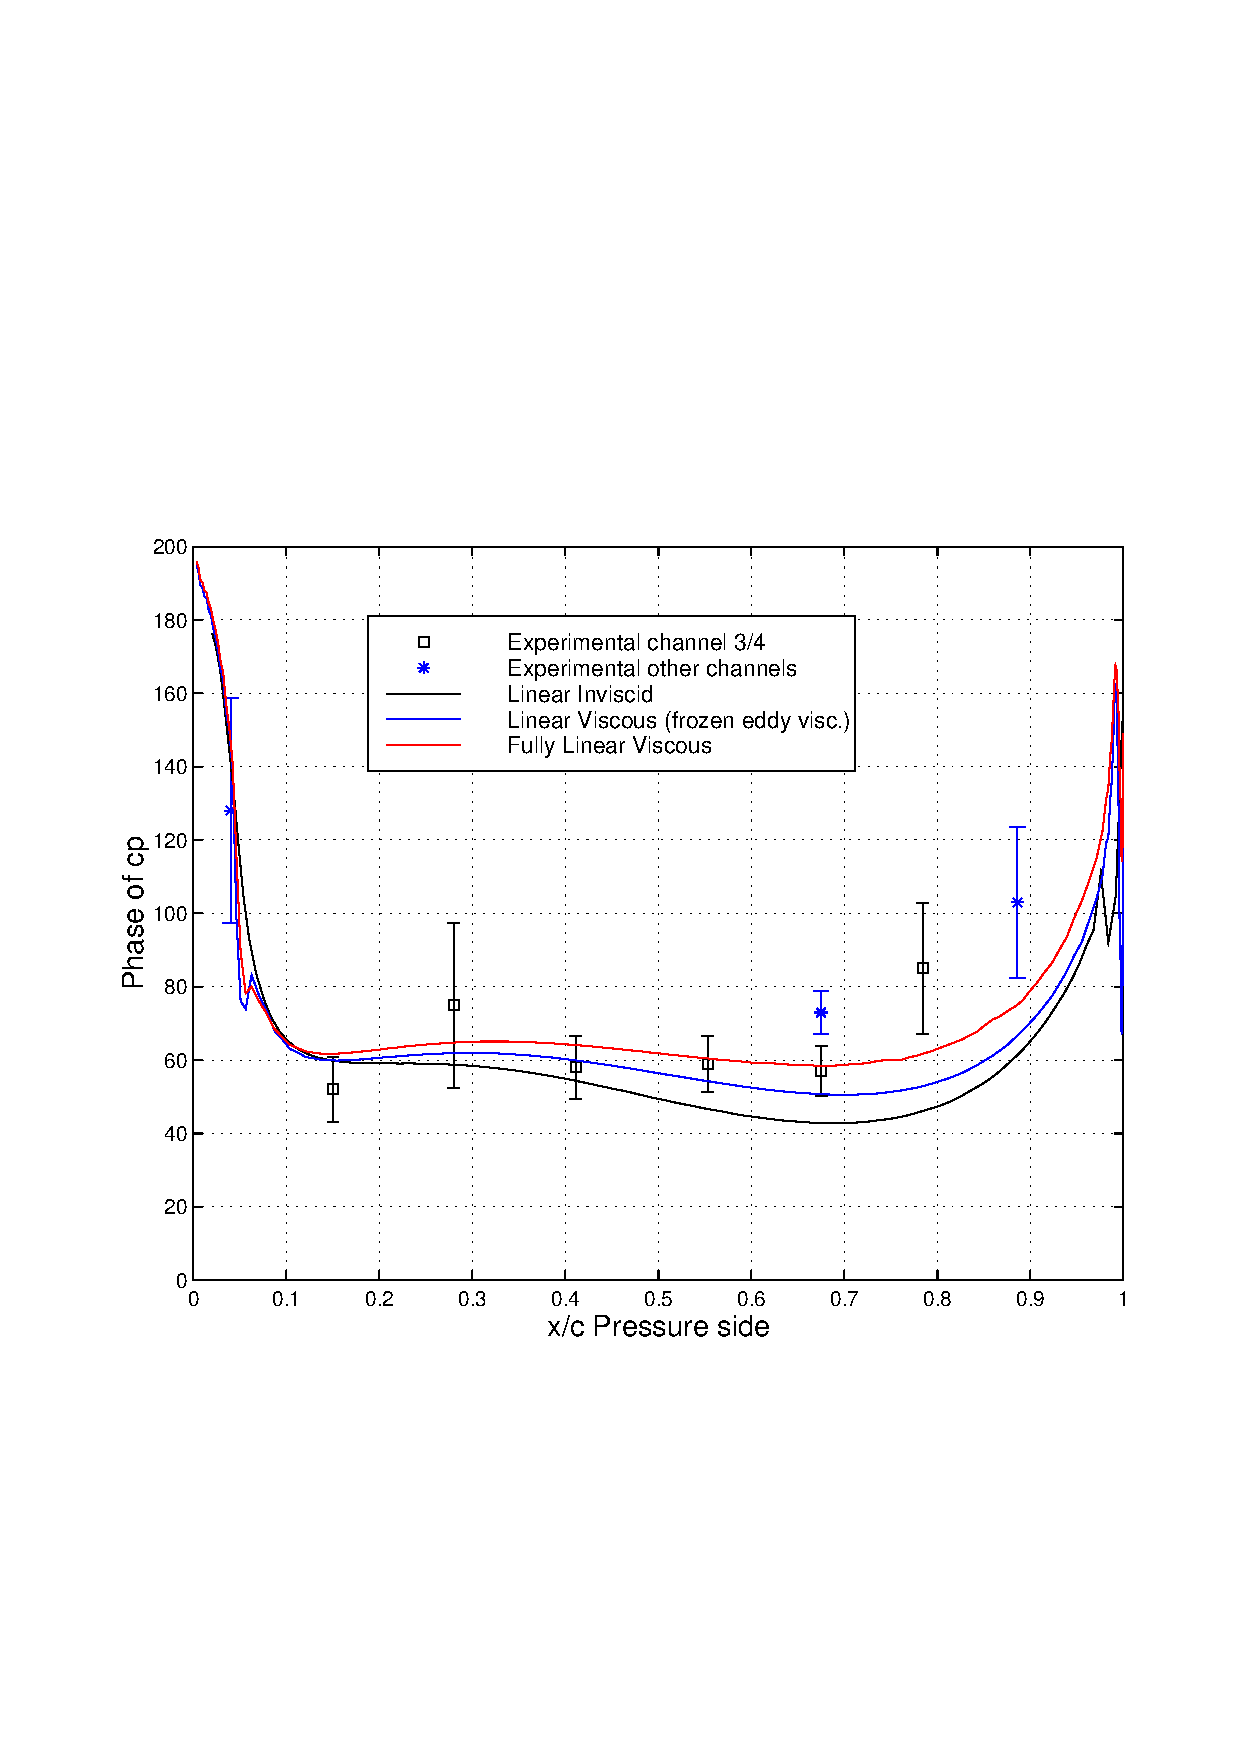
\includegraphics[height=100mm,clip=t]{CHAP_LINEAR/FIGURE/unsteady_blade_099_180_3.pdf}}\\
    {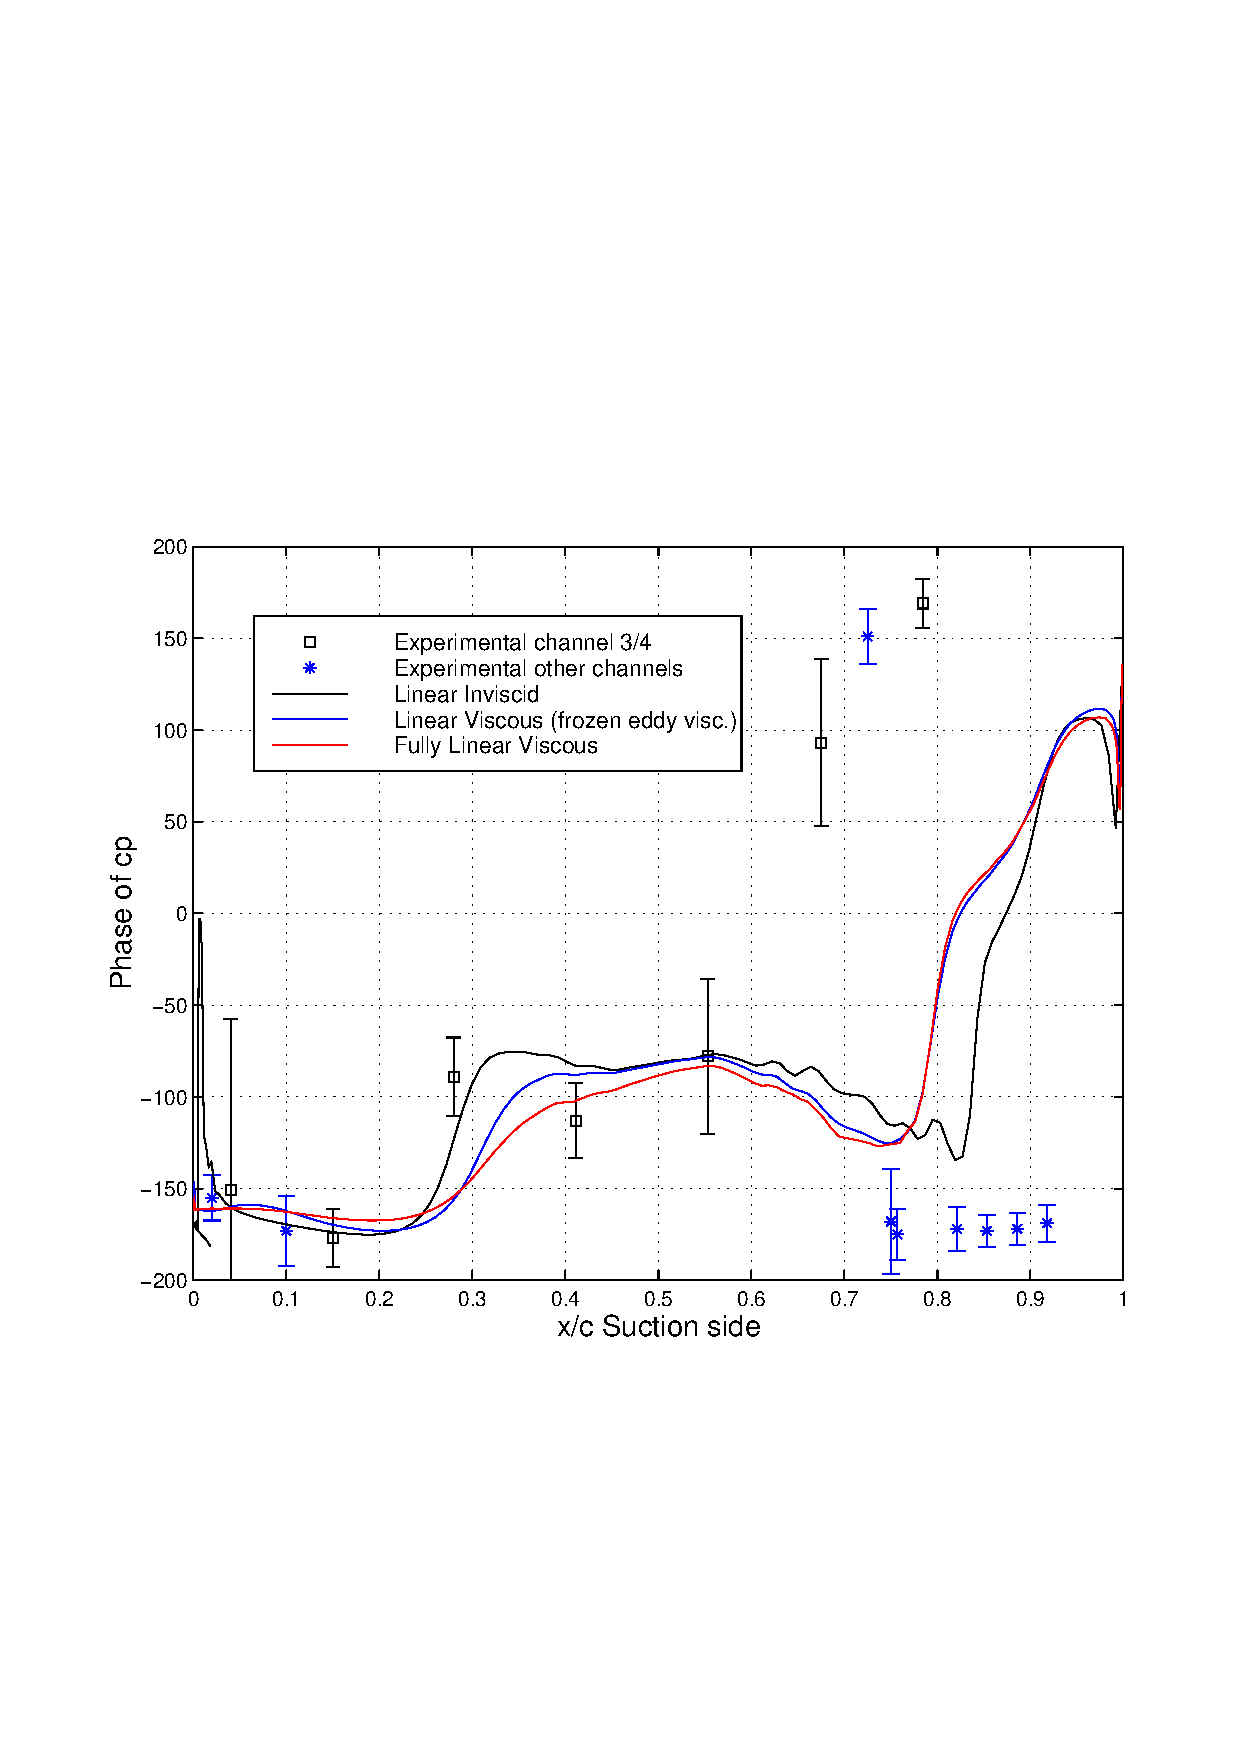
\includegraphics[height=100mm,clip=t]{CHAP_LINEAR/FIGURE/unsteady_blade_099_180_4.pdf}}
  \end{tabular}
 \end{center}
 \vspace{-7mm}
 \caption{$11^{th}$ Standard configuration - transonic case.
          Phase of of $\tilde{c}\sm{p}$
         ($\omega = 0.15$, $\phi = 180\se{o}$)}
 \label{transonic_11_phas.fig}
\end{figure}
%

%
%
\section{Concluding Remarks}
%
\begin{itemize}
%
\item
 A finite-volume scheme  has been presented for the solution of the linearised
 viscous flows for turbomachinery applications.
 The method employs an edge-based
 data structure and uses a nearest neighbour stencil for the discretisation of
 the Laplacian operator. Both 2D and 3D
 structured, unstructured or block structured grids with mixed elements 
 can be used without any modification of the numerical scheme. 
%
\item
 The proposed time-linearised Navier-Stokes analysis is applicable
 to off-design conditions  where viscous effects are not limited to the boundary layer.
%
\item
 The method is computationally very efficient, making it a useful tool for routine 
 aeroelasticity design calculations. For a given frequency and an interblade phase
 angle, the unsteady flow computation is about the same as the
 background steady-state flow computation.
 Although not reported in the main body of the Chapter, the time-linearised
 viscous analysis results for the $11\se{th}$ Standard Configuration
 are in very good agreement with the non-linear time-marching viscous predictions
 of Fransson et al. \citeyear{Bolcs:2}.
 It is anticipated that the non-linear computations will take about an order
 of magnitude longer. However, the issue whether linearised methods are applicable
 to all flow regimes is not one that is addressed here.
%
\item
 The  transonic flow results show that the linearisation of the turbulence model
 plays an important role wherever the viscous effects are important, exemplified
 here by the recirculation bubble. When there are no such effects, 
 the frozen turbulence approach should produce very similar results. In other words, 
 an inspection of the steady-state solution should provide guidance as to which
 modelling level would be appropriate.
%
\item
 Although only 2D cases are presented in this Chapter,
 3D flows have also been studied\footnote{An application to 3D fan flutter prediction
 is reported in Vahdati et al. \citeyear{Luca:12}.}
 albeit with a very significant increase in CPU effort.
 A fully-linearised turbulence model requires fine meshes near the wall,
 hence the problem size becomes much larger than those cases where a wall
 function is used. In such cases the unsteady shear stresses are neglected 
 so that a linearised wall function is not needed.
%
\end{itemize}
%
%
